% !TEX program = xelatex
% =====================================================================
% Seminar on Complex Multiplication
% A. Borel, S. Chowla, C. S. Herz, K. Iwasawa, J-P. Serre
% Lecture Notes in Mathematics 21, Springer-Verlag, 1966
%
% LaTeX 重排（依据《数学书籍LaTeX重排规范》）
% 编译：xelatex -> biber -> xelatex -> xelatex
% =====================================================================
\documentclass[11pt,oneside,openany,scheme=plain]{ctexbook}

% ---------- 页面 ----------
\usepackage[a4paper,left=3.0cm,right=3.0cm,top=3.0cm,bottom=3.2cm]{geometry}

% ---------- 数学宏包 ----------
\usepackage{amsmath,amssymb,amsthm,mathtools}
\usepackage{graphicx}
\usepackage{enumitem}
\usepackage{etoolbox}

% ---------- 颜色与超链接（与模板一致） ----------
\usepackage[dvipsnames]{xcolor}
\usepackage[
  colorlinks=true,
  linkcolor=MidnightBlue,
  citecolor=BrickRed,
  urlcolor=MidnightBlue,
  linktoc=all]{hyperref}

% ---------- 定理类环境 ----------
\theoremstyle{plain}
\newtheorem{theorem}{Theorem}
\newtheorem{proposition}{Proposition}
\newtheorem{lemma}{Lemma}
\newtheorem{corollary}{Corollary}
\theoremstyle{definition}
\newtheorem{definition}{Definition}
\newtheorem{example}{Example}
\theoremstyle{remark}
\newtheorem{remark}{Remark}

% hyperref 锚点唯一化（各章计数器显示文本允许重复，如 Corollary 1）
\renewcommand{\theHtheorem}{ch\arabic{chapter}.\arabic{theorem}}
\renewcommand{\theHproposition}{ch\arabic{chapter}.\arabic{proposition}}
\renewcommand{\theHlemma}{ch\arabic{chapter}.\arabic{lemma}}
\renewcommand{\theHcorollary}{ch\arabic{chapter}.\arabic{corollary}}

% 文字型陈述（原书编号不规则处：THEOREM IV'、Criterion、
% ARTIN RECIPROCITY LAW 等），标签文字与原书一致地写出。
\newenvironment{namedstmt}[1]{%
  \par\medskip\noindent\textbf{#1.}\enspace\ignorespaces}{\par\medskip}
% 参考文献条目的行内格式
\newcommand{\bibentry}[1]{\par\noindent\hangindent=2em\hangafter=1 #1\par\vspace{0.35em}}

% ---------- 章节样式 ----------
% 各章标题居中，编号为罗马数字 I--VIII，章题下附讲演者与日期一行，
% 均与原书版面一致。
\ctexset{
  chapter = {
    name = {},
    number = \Roman{chapter},
    format = {\centering\bfseries},
    aftername = {\hspace{1em}},
    beforeskip = -20pt,
    afterskip = 2.2em plus .1em,
    afterindent = false,
    pagestyle = fancy,
  },
  section = {
    name = {§,{.}},
    number = \arabic{section},
    aftername = {\hspace{0.6em}},
    format = {\bfseries},
    afterindent = false,
  },
  subsection = {
    afterindent = false,
  }
}

% 讲演者信息：\lecture{目录题}{章题}{讲演者}{日期}
% 章题排为原书的大写形式（如 I STATEMENT OF RESULTS），
% 其下居中排 "(Lecturer, Date)" 一行，均与原书版面一致。
\makeatletter
\newcommand{\lecture}[4]{%
  \chapter[#2]{\MakeUppercase{#2}}%
  \begin{center}\normalfont(#3, #4)\end{center}\vspace{0.6em}%
}
\makeatother

% ---------- 页眉页脚 ----------
\usepackage{fancyhdr}
\pagestyle{fancy}
\fancyhf{}
\renewcommand{\headrulewidth}{0pt}
\fancyhead[L]{\small\itshape Seminar on Complex Multiplication}
\fancyhead[R]{\small IAS, 1957--58}
\fancyfoot[C]{\thepage}
\fancypagestyle{plain}{%
  \fancyhf{}%
  \fancyfoot[C]{\thepage}%
  \renewcommand{\headrulewidth}{0pt}%
}
% frontmatter 用页脚中央页码
\newcommand{\frontpagestyle}{\pagestyle{plain}}

% ---------- 参考文献 ----------
\usepackage[
  backend=biber,
  sorting=nyt,
  hyperref=auto,
  backref=true,
  backrefstyle=three]{biblatex}
\addbibresource{refs.bib}

% ---------- 杂项 ----------
% 中文段落无缩进（本书正文为英文）
\setlength{\parindent}{1.5em}
\linespread{1.08}
\allowdisplaybreaks[2]

% 重排说明性注记
\newcommand{\typesetnote}[1]{}

\begin{document}

\frontmatter
% ---------- 扉页（与原书一致） ----------
\begin{titlepage}
  \centering
  \vspace*{1.5cm}
  {\large Lecture Notes in Mathematics\par}
  \vspace{0.6em}
  {\small An informal series of special lectures, seminars and reports on mathematical topics\par}
  \vspace{1.2em}
  {\small Edited by A.\ Dold, Heidelberg and B.\ Eckmann, Z\"urich\par}
  \vspace{3em}
  {\Large 21\par}
  \vspace{4em}
  {\normalsize A.\ Borel \textperiodcentered\ S.\ Chowla \textperiodcentered\ C.\ S.\ Herz\\
   K.\ Iwasawa \textperiodcentered\ J-P.\ Serre\par}
  \vspace{3em}
  {\huge Seminar\\[0.35em] on Complex Multiplication\par}
  \vspace{2.5em}
  {\small Seminar held at the Institute for Advanced Study, Princeton, N.J., 1957--58\par}
  \vspace{2em}
  {\normalsize 1966\par}
  \vfill
  Springer-Verlag \textperiodcentered\ Berlin \textperiodcentered\ Heidelberg \textperiodcentered\ New York
  \vspace{1.2em}

  {\large 译者\quad 翻译及重排\par}
\end{titlepage}

% 原书内封前的丛书说明（Lecture Notes 丛书宗旨，英文部分）
\noindent\frenchspacing
This series aims at speedy, informal, and high level information on new developments in mathematical research and teaching. Considered for publication are:
\begin{enumerate}[leftmargin=2.5em]
  \item Preliminary drafts of original papers and monographs
  \item Special lectures on a new field, or a classical field from a new point of view
  \item Seminar reports
  \item Reports from meetings
\end{enumerate}
Out of print manuscripts satisfying the above characterization may also be considered, if they continue to be in demand.

\medskip
The timeliness of a manuscript is more important than its form, which may be unfinished and preliminary. In certain instances, therefore, proofs may only be outlined, or results may be presented which have been or will also be published elsewhere.

\medskip
The publication of the ``Lecture Notes'' Series is intended as a service, in that a commercial publisher, Springer-Verlag, makes house publications of mathematical institutes available to mathematicians on an international scale. By advertising them in scientific journals, listing them in catalogs, further by copyrighting and by sending out review copies, an adequate documentation in scientific libraries is made possible.

\section*{Manuscripts}
Since manuscripts will be reproduced photomechanically, they must be written in clean typewriting. Handwritten formulae are to be filled in with indelible black or red ink. Any corrections should be typed on a separate sheet in the same size and spacing as the manuscript. All corresponding numerals in the text and on the correction sheet should be marked in pencil. Springer-Verlag will then take care of inserting the corrections in their proper places. Should a manuscript or parts thereof have to be retyped, an appropriate indemnification will be paid to the author upon publication of his volume. The authors receive $25$ free copies.

\medskip
Manuscripts in English, German or French should be sent to Prof.\ Dr.\ A.\ Dold, Mathematisches Institut der Universit\"at Heidelberg, Tiergartenstra\ss{}e or Prof.\ Dr.\ B.\ Eckmann, Eidgen\"ossische Technische Hochschule, Z\"urich.

\clearpage

% ==================== 目录 ====================
\tableofcontents


\mainmatter
% =====================================================================
% 第 I 章  Statement of results (J-P. Serre, Oct. 16, 1957)
% =====================================================================
\lecture{Statement of results}{Statement of Results}{J-P. Serre}{Oct. 16, 1957}

% ---------------------------------------------------------------
\section{The notion of complex multiplication}

Let $X$ be an elliptic curve. As a complex Lie group, it is the quotient
of the complex plane $\mathbb{C}$ by a lattice $\Gamma$, spanned by two
periods $\omega_{1}$, $\omega_{2}$, and since $X$ is isomorphic to the
curve defined by the periods $z\omega_{1}$, $z\omega_{2}$ for any non-zero
$z\in\mathbb{C}$, we may assume $\Gamma$ to be spanned by $1$ and $\tau$,
where $\tau$ has a positive imaginary part.

An endomorphism of $X$ may be identified with an endomorphism of its
universal covering $\mathbb{C}$ mapping $\Gamma$ into itself; it is
therefore the multiplication by a complex number $z$ such that
$z,\ z\tau\in\Gamma$. The endomorphisms of $X$ form a ring $A(X)$, which
always contains the integers $\mathbb{Z}$ (the ``trivial endomorphisms'').
The other ones (if any) are given by complex numbers and are called
\emph{complex multiplications}. If $A(X)\neq\mathbb{Z}$, the curve $X$ is
said to admit complex multiplications.

``In general'', $X$ has no complex multiplication. In fact, assume that
$z$ defines a non-trivial endomorphism of $X$. Then
\[
z=a+b\tau,\qquad z\tau=c+d\tau,\qquad(a,b,c,d\ \text{integers},\ b\neq 0),
\]
whence
\[
a\tau+b\tau^{2}=c+d\tau
\]
and $\tau$ must belong to an imaginary quadratic field, say $K$; moreover
$z$ belongs to the ring of integers $\mathfrak{o}(K)$ of $K$, since it is
in $K$ and defines an endomorphism of a $\mathbb{Z}$-module of finite
rank, namely $\Gamma$. Therefore, $A(X)$ is an \emph{order} of $K$
(subring of $\mathfrak{o}(K)$ containing $\mathbb{Z}$ and which has rank
$2$ as a $\mathbb{Z}$-module);

one gets in this way all orders of all quadratic imaginary fields (if $R$
is such an order, take for $X$ a curve with lattice of periods $R$; since
$1\in R$, $zR\subset R$ if and only if $z\in R$, whence $A(X)=R$).

Assume that $A(X)=\mathfrak{o}(K)$ and that $\Gamma\subset K$. Then
$\Gamma$ is an ideal of $K$, and conversely any ideal of $K$ gives rise
to a curve $X$ such that $A(X)=\mathfrak{o}(K)$. Two such curves are
isomorphic if and only if the corresponding ideals are homothetic,
i.e.\ belong to the same \emph{ideal class}.

Let $j$ be the modular function. For the curve with normal equation
\[
y^{2}=4x^{3}-g_{2}x-g_{3}
\]
its value is
\[
j=2^{6}\cdot 3^{3}\cdot g_{2}^{3}/\Delta,\qquad
(\Delta=g_{2}^{3}-27\cdot g_{3}^{2}\,).
\]

Two elliptic curves are isomorphic over an algebraically closed field if
and only if their modular invariants are equal. By the above, $j$ defines
a function on the ideal classes $\mathfrak{k}_{1},\ldots,\mathfrak{k}_{n}$
of $K$; the numbers $j(\mathfrak{k}_{i})$ are ``singular values'' of $j$,
and are called the \emph{class invariants} of $K$; they are pairwise
different, and have proved to be of fundamental importance in the study
of the abelian extensions of $K$, to which we now turn.

% ---------------------------------------------------------------
\section{Unramified abelian extensions of an imaginary quadratic field}

It is a classical result of Kronecker that every abelian extension
(i.e.\ normal extension with commutative Galois group) of the field
$\mathbb{Q}$ of rational numbers is contained in a field of roots of
unity. Thus, so to say, certain values of the exponential function
generate the maximal abelian extension of $\mathbb{Q}$. Such an
``explicit'' construction is also possible for an imaginary quadratic
field. One has to use the class invariants and also the values of a
certain function, related to the Weierstrass $\wp$-function
(see §\ref{sec:I-ramified}). This theory is essentially what is called
``complex multiplication''. We shall first deal with unramified
extensions. The results pertaining to this case may be embodied in the
following three theorems, where $K$ is an imaginary quadratic field,
$\mathfrak{k}_{i}$, $(1\leq i\leq h)$, its ideal classes.

\setcounter{theorem}{0}
\renewcommand{\thetheorem}{\Roman{theorem}}

\begin{theorem}\label{thm:I-one}
The class invariants $j(\mathfrak{k}_{i})$ are algebraic integers.
\end{theorem}

\noindent[Let us remark in passing that there is a sort of converse to
Theorem~\ref{thm:I-one}. Namely, C.~L. Siegel
(\emph{Transcendental numbers}, Annals of Math.\ Studies $16$,
Princeton, 1949, pp.~98--99) has deduced from certain results of
Schneider that if $z$ is an algebraic number in the upper half-plane not
belonging to a quadratic imaginary field, then $j(z)$ is transcendental.]

\begin{theorem}\label{thm:I-two}
$K(j(\mathfrak{k}_{i}))$ is independent of $i$, $(1\leq i\leq h)$, and is
the maximal unramified abelian extension of $K$.
\end{theorem}

\noindent(Unramified means that every prime ideal of $K$ decomposes in a
product of distinct prime ideals with exponents $1$.)

By class field theory, it is known that the maximal unramified abelian
extension of $K$ (Hilbert's ``absolute class field'') exists and that its
Galois group $G_{K}$ is canonically isomorphic to the group $C_{K}$ of
ideal classes; the next theorem describes how it operates on the
$j(\mathfrak{k}_{i})$.

\begin{theorem}\label{thm:I-three}
Let $\mathfrak{k}\in C_{K}$ and let $\sigma_{\mathfrak{k}}\in G_{K}$ be
its image by the isomorphism of class field theory. Then
\[
\sigma_{\mathfrak{k}}(j(\mathfrak{k}_{i}))
   =j(\mathfrak{k}^{-1}\cdot\mathfrak{k}_{i})\,.
\]
\end{theorem}

For the proofs of the above theorems, we shall follow the method of the
first part of Hasse's paper quoted in §5, which presupposes class-field
theory. More specifically, Hasse establishes by function theoretical
arguments Theorem~\ref{thm:I-one} and the congruence
\[
j(\mathfrak{p}^{-1}\cdot\mathfrak{k})
   \equiv j(\mathfrak{k})^{N\mathfrak{p}}\mod \mathfrak{p}
\tag{1}\label{eq:I-1}
\]
($\mathfrak{p}$ prime ideal of $K$, $\mathfrak{k}$ ideal class,
$N\mathfrak{p}$ absolute norm of $\mathfrak{p}$), for almost all
(i.e.\ all but a finite number of) prime ideals of $K$ having absolute
degree one (i.e.\ $N\mathfrak{p}=p$ with $p$ prime) with respect to
$\mathbb{Q}$. The validity of \eqref{eq:I-1} for all $\mathfrak{p}$ and
Theorems~\ref{thm:I-two}, \ref{thm:I-three} will then follow by class
field theory.

% ---------------------------------------------------------------
\section{Algebraic interpretation}

For any complex number $j$, there is an elliptic curve $X$ defined over
$\mathbb{Q}(j)$, with invariant $j$; it may for instance be given by the
equation
\[
y^{2}=4x^{3}-h(x+1),\qquad\bigl(h=27j\,(j-2^{6}\!\cdot 3^{3})^{-1}\bigr).
\]

If in particular $j=j(\mathfrak{k})$, with $K,\mathfrak{k}$ as before,
then $K(j)$ is the smallest field of definition for all elements of
$A(X)$. From this, it follows easily that the numbers $j(\mathfrak{k}_{i})$
are algebraic and that $L=K(j(\mathfrak{k}_{i}))$ is independent from
$i$.

Moreover, given a prime ideal $\mathfrak{p}$ of $K$, there is an
algebraic procedure to obtain from $X$ a curve, call it $X_{\mathfrak{p}}$,
with invariant $j(\mathfrak{p}^{-1}\cdot\mathfrak{k})$, also defined over
$K(j)$.

Deuring's method relies on the notion of reduction of $X$ modulo a prime
ideal $\mathfrak{q}$ of $L$. This means that we consider the curve with
the same equation as $X$, but the coefficients being reduced mod
$\mathfrak{q}$. It may be shown that for almost all $\mathfrak{q}$, this
is possible and leads to an elliptic curve $\bar{X}$ which does not depend
on the particular equation chosen to define $X$. The curve $\bar{X}$ is
then defined over a field of characteristic $p$, where $p$ is the prime
number contained in $\mathfrak{q}$.

To any algebraic variety $V$ defined over a field of characteristic
$p\neq 0$, one can associate its ``$p$-th power'' $V^{p}$. Roughly
speaking, $V^{p}$ is obtained by raising to the $p$-th power all
coordinates of the points in any affine model of $V$. In particular we can
consider $\bar{X}^{\mathfrak{q}}$ for any $q=p^{s}$ ($s$ positive integer).

With these notations, Deuring proves by a simple argument that the equality
\[
\bar{x}^{N\mathfrak{p}}=\overline{(x_{\mathfrak{p}})\,},\qquad
(\mathfrak{p}=K\cap\mathfrak{q}),
\tag{3}\label{eq:I-3}
\]
holds for almost all $\mathfrak{p}$ of degree $1$, whence the congruence
\eqref{eq:I-1}.

So far, it has not been possible to prove along these lines that the
class invariants are integral numbers. Deuring's proof for this fact is
the analogue with formal power series of the classical argument.

% ---------------------------------------------------------------
\section{Ramified extensions}\label{sec:I-ramified}

Let as before $K=\mathbb{Q}(\sqrt{-d})$ ($d$ positive square-free
integer) be a quadratic imaginary field, and $X$ an elliptic curve with
invariant $j=j(\mathfrak{k})$, where $\mathfrak{k}$ is an ideal class of
$K$. Its group of automorphisms $\operatorname{Aut} X$ is the group of
units of $A(X)$, i.e.\ of $\mathfrak{o}(K)$. This group is cyclic of
order $2$ (resp.\ $4$, resp.\ $6$) when $d\neq 1,3$ (resp.\ $d=1$,
resp.\ $d=3$).

The quotient $X'$ of $X$ by $\operatorname{Aut} X$ is an algebraic curve
(of genus zero), defined over $K(j)$.

Since $X$ is a group variety, defined over $K(j)$, its points of order
$n$ will be algebraic and so will be their images in $X'$. We can now
state the main theorem of complex multiplication for ramified extensions:

\begin{theorem}\label{thm:I-four}
Let $K$ be an imaginary quadratic field, $j$ a class invariant of $K$,
and $X$ an elliptic curve with modular invariant $j$ defined over
$L=K(j)$. The maximal abelian extension of $K$ can then be obtained by
adjoining to $L$ the coordinates in $X'=X/\operatorname{Aut}X$ of all
points of order $n$ of $X$ $(n=1,2,\ldots)$.
\end{theorem}

In order to express Theorem~\ref{thm:I-four} analytically, we introduce
the function
\[
\tau(u;\omega_{1},\omega_{2})
=(-1)^{e/2}\,\wp^{e/2}(u;\omega_{1},\omega_{2})\,
g^{(e)}(\omega_{1},\omega_{2})
\]
where $e=\text{order }\operatorname{Aut}X$, $\wp(u;\omega_{1},\omega_{2})$
is the Weierstrass function,
\[
\begin{gathered}
g^{(2)}=2^{7}\cdot 3^{5}\,g_{2}\,g_{3}/\Delta\\
g^{(3)}=2^{8}\cdot 3^{4}\,g_{2}^{2}/\Delta\\
g^{(6)}=2^{9}\cdot 3^{6}\,g_{3}/\Delta\,.
\end{gathered}
\]

We have then:
\begin{namedstmt}{THEOREM IV$'$}
Let $K$ be an imaginary quadratic field, $j$ a class invariant of $K$,
$\omega_{1}$, $\omega_{2}$ a basis for some ideal of $K$. Then the maximal
abelian extension of $K$ may be obtained by adjoining to $L=K(j)$ the
numbers
$\tau\bigl((a\omega_{1}+b\omega_{2})/n;\omega_{1},\omega_{2}\bigr)$,
$(a,b,n\in\mathbb{Z},\ n>0)$.
\end{namedstmt}

The maximal abelian extension of $K$ can also be obtained by adjoining
to $K$ the roots of unity, the values $j(z)$ of the modular function for
all $z\in K^{*}$ having positive imaginary part, and square roots of
elements in the field thus obtained. For this and its relation to the
so-called Kronecker Jugendtraum, see Hasse's \emph{Klassenk\"orper
Bericht}
\cite{hasse1926bericht}, §10.

% ---------------------------------------------------------------
\section{Bibliographical notes}\label{sec:I-notes}

We content ourselves with some brief indications, without making any
attempt towards completeness. As to the 19-th century literature, we just
quote \cite{kroneckerWerke}.

The first two systematic and detailed accounts are to be found in
\cite{weber1908algebra,fueter1924moduln,fueter1927moduln}.

Weber's book contains most of the essential results. However, although
Weber already introduces and obtains several properties of the function
$\tau$, both he and Fueter have to use other, more complicated, functions
to generate the maximal abelian extension. That this could be performed
by means of $\tau$ only was first shown by Hasse
\cite{hasse1927neue,hasse1931neue}.

Teil II and the above mentioned books follow the analytical method.
Hasse's Teil I combines analysis and class field theory.

The purely algebraic approach was initiated and carried out by
M.~Deuring. See notably \cite{deuring1947algebraische,deuring1952struktur}.

It was clear from the outset that a main obstacle to a generalization of
Deuring's methods to higher dimensional abelian varieties was the lack of
a good theory for reduction mod $\mathfrak{p}$ in algebraic geometry.
This was recently supplied by Shimura \cite{shimura1955reduction}
(Amer.\ Jour.\ Math.\ 77, 134--176 (1955)), and was applied to higher
dimensional extensions of complex multiplication by Shimura, Taniyama,
Weil. See \cite{shimura1955tokyo,taniyama1955tokyo,weil1955tokyo}.

The two-dimensional case had been considered long ago by Hecke (following
a suggestion of Hilbert), using analytical methods. See
\cite{hecke1912hohere,hecke1913konstruktion}.

[(Added in 1965). The Shimura--Taniyama--Weil theory has been published:
\cite{shimuramataniyama1961}. A systematic exposition of the analytic
method is given in \cite{deuringklassenkorper}. For further results, see
\cite{ramachandra1964applications}.]

% =====================================================================
% 第 II 章  Modular forms (J-P. Serre, Oct. 23 and 30, 1957)
% =====================================================================
\lecture{Modular forms}{Modular Forms}{J-P. Serre}{Oct. 23 and 30, 1957}

\setcounter{proposition}{0}
\setcounter{lemma}{0}
\setcounter{corollary}{0}

% ---------------------------------------------------------------
\section{The modular group}

Let $E\subset\mathbb{C}$ be the upper half plane $\operatorname{Im}(w)>0$;
the \emph{modular group} $G$ is the group of automorphisms of $E$ of the form
\[
w\longrightarrow\frac{aw+b}{cw+d}
\]
\[
(a,b,c,d\in\mathbb{Z},\ ad-bc=1).
\]
This group is the factor group of $\mathrm{SL}(2,\mathbb{Z})$ by its center
$\{\pm 1\}$.

Let now $\Gamma$ be a lattice in $\mathbb{C}$; we can choose two generators
$w_{1},w_{2}$ of $\Gamma$ such that $w_{1}\wedge w_{2}<0$; they are
determined up to a transformation of $\mathrm{SL}(2,\mathbb{Z})$. If we then
put $w=w_{1}/w_{2}$, we have $w\in E$, and the orbit of $w$ under $G$ does
not depend on the choice of $w_{1}$, $w_{2}$. Two lattices $\Gamma$ and
$\Gamma'$ correspond to the same orbit if and only if they are homothetic,
i.e.\ if the elliptic curves $\mathbb{C}/\Gamma$ and $\mathbb{C}/\Gamma'$
are isomorphic. Conversely, every orbit $Gw$ corresponds to some lattice
(for instance, $\Gamma=\mathbb{Z}+w\mathbb{Z}$). Hence:

\begin{proposition}\label{prop:II-1}
The isomorphism classes of elliptic curves are in one-to-one
correspondence with the orbits of $G$ in $E$.
\end{proposition}

We denote by $X$ the set $E/G$ of the orbits of $G$ in $E$. Our first task
is to find a well-behaved set of representatives for $X$ in $E$.

% ---------------------------------------------------------------
\section{Fundamental domain for the modular group}

Let $T$ be the translation $w\longrightarrow w+1$, and $S$ the
``inversion-symmetry'' $w\longrightarrow -\frac{1}{w}$; one has $T,S\in G$
and $S^{2}=1$.

\begin{proposition}\label{prop:II-2}
Let $D=\{w\mid w\in E,\ |\operatorname{Re}w|\leq\tfrac{1}{2},\ |w|\geq 1\}$.
Any orbit of $G$ meets $D$. Moreover, two distinct points $w$ and $w'$ of
$D$ are equivalent under $G$ if and only if either $w'=T^{\pm 1}w$,
$\operatorname{Re}w'=\pm\tfrac{1}{2}$ or $w'=Sw$, $|w|=1$. The set $D$ is
called a ``fundamental domain'' of the modular group $G$.
\end{proposition}

\begin{proposition}\label{prop:II-3}
The group $G$ is generated by $S$ and $T$.
\end{proposition}

\begin{figure}[htbp]
  \centering
  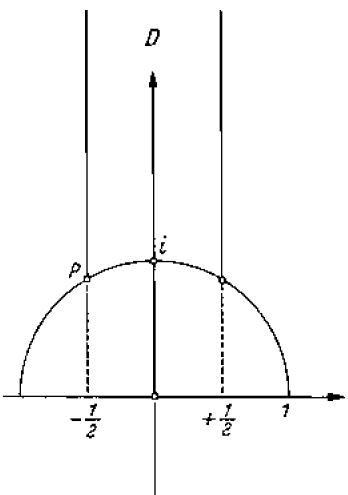
\includegraphics[width=0.42\linewidth]{figures/ch2-fundamental-domain.jpg}
  \label{fig:II-domain}
\end{figure}

\begin{proposition}\label{prop:II-4}
The stability group of $\rho=e^{2\pi i/3}$ (resp.\ of $i$) is of order
$3$ (resp.\ of order $2$), and is generated by $Q=ST$ (resp.\ by $S$).
Conversely, any point of $E$ with a non-trivial stability group is
equivalent under $G$ to either $\rho$ or $i$.
\end{proposition}

These three propositions will be proved at the same time. If
$w'=Aw=\frac{aw+b}{cw+d}$, a simple computation shows that:
\[
\operatorname{Im}(w')=\operatorname{Im}(w)/|cw+d|^{2}.
\tag{1}\label{eq:II-1}
\]

For a fixed $w\in E$, the set of all $cw+d$ ($c,d\in\mathbb{Z}$) is
discrete; hence, the $\operatorname{Im}(w')$ have no non-zero accumulation
point. Let then $G'$ be the subgroup of $G$ generated by $S$ and $T$, and
let $G'w$ be any orbit of $G'$ in $E$. By the above, we can assume that
$\operatorname{Im}(w)$ is maximum on $G'w$; formula \eqref{eq:II-1},
applied with $A=S$, gives $|w|\geq 1$. On the other hand,
$|\operatorname{Re}(T^{n}w)|\leq\frac{1}{2}$ for a suitable
$n\in\mathbb{Z}$; since $T$ does not change imaginary parts,
$\operatorname{Im}(T^{n}w)=\operatorname{Im}(w)$, and therefore
$T^{n}w\in D$. Thus, every orbit of $G'$ meets $D$.

Let now $w$ and $w'=Aw$ $(A\in G,\ A\neq 1)$ be points of $D$, with
$\operatorname{Im}(w')\geq\operatorname{Im}(w)$. Formula \eqref{eq:II-1}
then yields $|cw+d|\leq 1$, and, since we can assume $c\geq 0$, it follows
that $c=0$, $1$. If $c=0$, then $a=d=\pm 1$, $w'=w+b$, whence $b=\pm 1$
and $\operatorname{Re}w=\mp\frac{1}{2}$. If $c=1$, then we must have
$|w|=1$, $d=0$, unless $w$ is equal to $\rho$ or $\rho+1$, in which case
$d=0,1$ or $d=0,-1$. The formula $d=0$ gives
$w'=a-\frac{1}{w}=T^{a}Sw$. Since $Sw\in D$, the first part of the
discussion gives $a=0$, except when $\operatorname{Re}(Sw)=\pm\frac{1}{2}$,
i.e.\ $w=\rho$ or $\rho+1$; when $w=\rho$, one can take $a=-1$, and,
similarly for $w=\rho+1$. Finally, the formulas $w=\rho$, $d=1$ imply
$w'=a-1/(\rho+1)=a+\rho$, whence $a=0,1$.

Propositions \ref{prop:II-2} and \ref{prop:II-4} follow readily from this
discussion.

Let now $A\in G$, and let choose a point $w$ in the interior of $D$; the
orbit of $Aw$ under $G'$ meets $D$. Hence, there exists $B\in G'$ such
that $BAw\in D$. By propositions \ref{prop:II-2} and \ref{prop:II-4}, we
have $BA=1$, hence $A\in G'$, and proposition \ref{prop:II-3} is proved.

\subsection*{Remarks.}

\noindent
1) It is possible to prove (for instance, by topological arguments) that
the relations between $S$ and $T$ are generated by $(ST)^{3}=1$. Hence,
the modular group $G$ is isomorphic to the free product of a cyclic group
of order $2$ (corresponding to $S$) and a cyclic group of order $3$
(corresponding to $ST$).

\medskip\noindent
2) Let $Q(x,y)=Ax^{2}+Bxy+Cy^{2}$ be a positive definite binary quadratic
form, with real coefficients. Such a form can be written:
\[
Q(x,y)=|xw_{1}+yw_{2}|^{2},
\]
for a suitable choice of $w_{1}$, $w_{2}$. Applying proposition
\ref{prop:II-2} to $w=w_{1}/w_{2}$, one then obtains the existence of a
form $Q'=A'x^{2}+B'xy+C'y^{2}$ which is equivalent to $Q$ under the group
$\mathrm{SL}(2,\mathbb{Z})$, and verifies the inequalities:
\[
A'\geq C'\geq|B'|.
\]
[This ``reduction'' process was already given in Gauss's
\emph{Disquisitiones arithmeticae}.]

% ---------------------------------------------------------------
\section{Analytic structure and compactification of X=E/G}\label{sec:II-analytic}

We will first prove that the group $G$ is ``discontinuous'' in $E$:

\begin{proposition}\label{prop:II-5}
Let $K$ be a compact subset of $E$. Then:

(i) There exists a number $N$ such that $\operatorname{Im}(Aw)<N$ for
every $A\in G$ and $w\in K$.

(ii) For every compact subset $K'$ of $E$, the set of $A\in G$ such that
$AK\cap K'\neq\emptyset$ is finite. [i.e.\ $\lim AK=\infty$].
\end{proposition}

Statement (i) follows from formula \eqref{eq:II-1} and the fact that
$\inf|cw+d|>0$, when $w$ runs through $K$, and $c,d$ run through all pairs
of relatively prime integers.

Statement (ii) does in fact hold for every discrete subgroup of
$\mathrm{SL}(2,\mathbb{R})/\{\pm 1\}$. In the case of the modular group
$G$, it can be checked in the following way:

Formula \eqref{eq:II-1} shows that the number of pairs $(c,d)$ associated
with transformations $A\in G$ such that $AK\cap K'\neq\emptyset$ is
finite. But two elements $A_{1},A_{2}\in G$ have the same $(c,d)$ if and
only if $A_{1}=T^{n}A_{2}$ with some $n\in\mathbb{Z}$. Since
$T^{n}A_{2}K$ tends to $\infty$ with $n$, one has
$T^{n}A_{2}K\cap K'\neq\emptyset$ only for a finite number of values of
$n$, and (ii) follows immediately.

\begin{corollary}\label{cor:II-hausdorff}
The factor space $X=E/G$ is Hausdorff (and hence locally compact).
\end{corollary}

This is a formal consequence of (ii):

Let $w$ and $w'$ in $E$ be inequivalent under $G$. Since $Aw'\to\infty$,
there exists a compact neighbourhood $U$ of $w$ such that $Aw'\notin U$
for any $A\in G$. Let $V$ be a compact neighbourhood of $w'$ and
$N\subset G$ be the set of all $A$ such that $AV\cap U\neq\emptyset$; by
(ii), the set $N$ is finite. For any $A\in N$, let $W_{A}$ be a
neighbourhood of $Aw'$ which does not meet $U$, and put
$U'=V\cap\bigcap_{A\in N}A^{-1}W_{A}$; the set $U'$ is a neighbourhood of
$w'$. If $A\in N$, one has $AU'\subset W_{A}$ hence
$AU'\cap U=\emptyset$; if $A\notin N$, one has $AU'\subset AV$ hence again
$AU'\cap U=\emptyset$. This means that $GU$ and $GU'$ are disjoint
saturated neighbourhoods of the orbits $Gw$ and $Gw'$, q.e.d.

\begin{corollary}\label{cor:II-proper}
The canonical projection of the fundamental domain $D$ onto $X$ is proper.
\end{corollary}

If $K$ is a compact subset of $E$, one has to show that
$B=\bigcup_{A\in G}AK\cap D$ is compact. Property (ii) shows that
$\bigcup AK$ is locally finite, hence closed; on the other hand, property
(i) shows that $\operatorname{Im}(w)$ is bounded for $w\in B$. The set
$B$, being closed and bounded, is therefore compact.

\begin{corollary}\label{cor:II-homeo}
Let $R$ be the equivalence relation induced on $D$ by the equivalence
under $G$ (the relation $R$ has been given explicitly in prop.\
\ref{prop:II-2}). The canonical projection $D\to X$ induces an
homeomorphism of $D/R$ onto $X$.
\end{corollary}

The map $D/R\longrightarrow X$ is bijective (prop.~\ref{prop:II-2}),
continuous, and proper (follows from cor.~\ref{cor:II-proper}). Since both
$D/R$ and $X$ are locally compact, it is a homeomorphism.

After these preliminaries, we define an analytic structure on $X$ in the
following way:

Let $p:E\longrightarrow X$ denote the canonical projection. A continuous
function $f$ on an open set $U$ of $X$ is said to be holomorphic if
$f\circ p$ is holomorphic on $p^{-1}(U)$. One checks easily that the
axioms of a complex analytic structure are verified: if $P\in E$ is a
point of order $e$ (i.e.\ the stability group $G_{P}$ of $P$ is of order
$e$), we can find a local parameter $z_{P}$ around $P$ such that $G_{P}$
operates on $z_{P}$ by multiplication by $e$-th roots of unity, and
$(z_{P})^{e}$ is a local parameter around $p(P)\in X$ [one can take for
instance $z_{P}=(w-P)/(w-\bar{P})$].

Let now $\hat{X}=X\cup\{\infty\}$ be the one-point compactification of
$X$; we now want to extend to $\hat{X}$ the analytic structure of $X$.
Let $E_{1}$ be the half plane $\operatorname{Im}(w)>1$; it follows from
formula \eqref{eq:II-1} that the equivalence relation induced on $E_{1}$
by $G$ is given by the translations $T^{n}$. One has therefore
$p(E_{1})\approx E_{1}/T$; but the mapping $w\longrightarrow
q=e^{2\pi iw}$ is an analytic isomorphism of $E_{1}/T$ onto some open disk
(minus the origin); putting $q(\infty)=0$, we then extend $q$ to
$p(E_{1})\cup\{\infty\}$, and take this function as a local parameter
around $\infty$ on $\hat{X}$. This gives the desired extension. A
meromorphic function on $\hat{X}$ may therefore be defined as a
meromorphic function on $E$, invariant under $G$, admitting a power series
expansion $\sum_{n\geq k}a_{n}q^{n}$ which converges around $q=0$. Such a
function is called a \emph{modular function}.

\begin{proposition}\label{prop:II-6}
The space $\hat{X}$ is analytically isomorphic to the sphere
$S_{2}=\hat{\mathbb{C}}$.
\end{proposition}

By cor.~\ref{cor:II-homeo} to prop.~\ref{prop:II-3}, $X$ is homeomorphic
to $D/R$, i.e.\ to a plane. The Riemann surface $\hat{X}$ is therefore
homeomorphic to $S_{2}$, and, as is well known, this implies that it is
analytically isomorphic to $S_{2}$.

If $\lambda:\hat{X}\longrightarrow\hat{\mathbb{C}}$ is an analytic
isomorphism, every modular function is a rational function of $\lambda$.
Such a $\lambda$ is determined up to an analytic automorphism of
$\hat{\mathbb{C}}$; we normalize it by asking that it maps $\infty$ and
$p(\rho)$ on-to $\infty$ and $0$ respectively, and has residue equal to
$1$ at $\infty$ (when expanded in a power series of $q$). This particular
choice of $\lambda$ will be referred to as ``the'' modular function, and
be denoted by $j$.

\noindent\emph{Note.} Proposition \ref{prop:II-6} means that $X$ is
analytically isomorphic to $\mathbb{C}$. This can also be proved by using
the fact that the ``half fundamental domain''
$D_{+}=\{w\mid 0<\operatorname{Re}w<\frac{1}{2},\ |w|>1\}$ is analytically
isomorphic to a half plane, and applying Schwarz's symmetry principle.

% ---------------------------------------------------------------
\section{Modular functions of weight k}\label{sec:II-weight}

A (meromorphic) modular function of weight $k$ ($k\in\mathbb{Z}$) is a
meromorphic function $h$ on $E$ such that:
\[
h(Aw)=(cw+d)^{2k}h(w)\qquad(A\in G),
\tag{2}\label{eq:II-2}
\]
and which admits a Laurent expansion in $q=e^{2\pi iw}$ with a finite
number of negative exponents:
\[
h=\sum\nolimits_{n\geq k}a_{n}q^{n}.
\]

A function of weight $0$ is thus a modular function in the sense of
§\ref{sec:II-analytic}. A modular function of weight $k$ which is
holomorphic in $E$ and at $\infty$ is called a \emph{modular form}.

Equation \eqref{eq:II-2} is equivalent to the fact that the function of
$w_{1},w_{2}$ defined by:
\[
h(w_{1},w_{2})=w_{2}^{-2k}h(w_{1}/w_{2})
\]
is invariant under the group $\mathrm{SL}(2,\mathbb{Z})$; note that
$h(w_{1},w_{2})$ is homogeneous of degree $-2k$.

Since $d\bigl(\frac{aw+b}{cw+d}\bigr)=dw/(cw+d)^{2}$, one can also express
\eqref{eq:II-2} by saying that the differential form of degree $k$
$\omega=h\,dw^{k}$ is invariant by $G$, and hence represents a differential
form on $\hat{X}$. The condition that $h$ be meromorphic on $E$ and at
$\infty$ means that $\omega$ is everywhere meromorphic on $\hat{X}$. More
precisely:

\begin{proposition}\label{prop:II-7}
Let $\omega=h\,dw^{k}$ be the differential form on $\hat{X}$ associated
with the modular function $h$ of weight $k$. For any point $P\in E$, let
$w_{P}(h)$ denote the order of $h$ at $P$ and $v_{P}(\omega)$ the order of
$\omega$ at the corresponding point of $\hat{X}$; let $w_{\infty}(h)$ and
$v_{\infty}(\omega)$ be defined similarly. Then:
\[
w_{\infty}(h)=v_{\infty}(\omega)+k,
\tag{3}\label{eq:II-3}
\]
\[
w_{P}(h)=e\cdot v_{P}(\omega)+k(e-1)\qquad(e=\text{order of }P).
\tag{4}\label{eq:II-4}
\]
\end{proposition}

Equation \eqref{eq:II-3} follows immediately from the relation
$2\pi i\,dw=\frac{dq}{q}$. For $P\in E$, choose a local parameter $z_{P}$
such that the isotropy group $G_{P}$ operates on $z_{P}$ by multiplication
by $e$-th roots of unity, and let $t=(z_{P})^{e}$. We can then write:
\[
\begin{gathered}
\omega=u\,t^{N}dt^{k}\quad(u\ \text{holomorphic}\neq 0,\ N=v_{P}(\omega)),\\
\omega=u\,e^{k}(z_{P})^{Ne+k(e-1)}(dz_{P})^{k},
\end{gathered}
\]
which yields \eqref{eq:II-4}.

On an algebraic curve of genus $g$, the sum of the orders of a
differential form of degree $k$ is equal to $k(2g-2)$. Here $g=0$. Hence:

% 原书中命题 7 的两条推论编号重新从 1 开始（Corollary 1, 2）。
\setcounter{corollary}{0}
\xdef\theHcorollary{ch2.blockB.\arabic{corollary}}
\begin{corollary}\label{cor:II-valence}
If $h$ is a modular function of weight $k$, one has:
\[
w_{\infty}(h)+\frac{1}{2}w_{i}(h)+\frac{1}{3}w_{\rho}(h)
+\Sigma^{*}\,w_{P}(h)=\frac{k}{6},
\tag{5}\label{eq:II-5}
\]
where $\Sigma^{*}$ means that $P$ runs through a set of representatives
of the equivalence classes of ordinary points (i.e.\ points of order $1$).
\end{corollary}

\noindent[Formula \eqref{eq:II-5} can also be proved directly by
integrating $dh/h$ over the boundary of $D$.]

Let $M_{k}$ denote the vector space of modular forms of weight $k$. If $h$
is a non-zero element of $M_{k}$, one has $w_{P}(h)\geq 0$ for all
$P\in E$ and also $w_{\infty}(h)\geq 0$. Formula \eqref{eq:II-5} then
shows that $k\geq 0$. For $k=0$, the only elements of $M_{k}$ are the
constants; for $k=1$, formula \eqref{eq:II-5} shows that $M_{k}=0$. For
$k=2$, one sees that every non-zero element $h\in M_{k}$ has a zero only
on the orbit of $\rho$, and that these zeros are simple; if $h'\in M_{2}$,
a suitable linear combination $h'-ah$ has a zero outside this orbit, hence
is identically zero; this shows that $\dim M_{2}\leq 1$. An analogous
result holds for $M_{3}$ with $i$ replacing $\rho$. We have proved:

\begin{corollary}\label{cor:II-dim}
a) $M_{k}=0$ for $k<0$ and for $k=1$.

b) $\dim M_{k}\leq 1$ for $k=2,3$.

c) If $h$ is a non-zero element of $M_{2}$ (resp.\ $M_{3}$), it has zeros
only on the orbit of $\rho$ (resp.\ of $i$), and these zeros are simple.
\end{corollary}

% ---------------------------------------------------------------
\section{Eisenstein series}\label{sec:II-eisenstein}

Let $\Gamma=\mathbb{Z}w_{1}+\mathbb{Z}w_{2}$ be a lattice in
$\mathbb{C}$, and let $k$ be an integer, with $k\geq 2$. The Eisenstein
series $G_{k}(\Gamma)$ of degree $k$ associated to $\Gamma$ is defined by
the formula:
\[
G_{k}(\Gamma)=\sum_{u\in\Gamma-\{0\}}\frac{1}{u^{2k}}
=\!\!\sum_{\substack{m,n\in\mathbb{Z}\\(m,n)\neq(0,0)}}\!\!
(mw_{1}+nw_{2})^{-2k}.
\tag{6}\label{eq:II-6}
\]

The series $G_{2}$ and $G_{3}$ are identical (up to a constant factor)
with the $g_{2}$ and $g_{3}$ of Weierstrass's theory:
\[
g_{2}=60\,G_{2},\qquad g_{3}=140\,G_{3}.
\]

To the homogeneous function $G_{k}(w_{1},w_{2})=G_{k}(\Gamma)$ is
associated a function $G_{k}(w)$ of $w=w_{1}/w_{2}$ by the formula:
\[
G_{k}(w)=(w_{2})^{2k}G_{k}(w_{1},w_{2})
=\sum_{\substack{m,n\in\mathbb{Z}\\(m,n)\neq(0,0)}}(m+nw)^{-2k}.
\tag{8}\label{eq:II-8}
\]

\begin{proposition}\label{prop:II-8}
For $k\geq 2$, the series \eqref{eq:II-8} is absolutely convergent in $E$
and normally convergent in $D$. Its sum $G_{k}(w)$ is a modular form of
weight $k$ whose value at infinity is equal to $2\zeta(2k)$.
\end{proposition}

In $D$, we have $|\operatorname{Re}(w)|\leq\frac{1}{2}$ and
$|w|\geq 1$, whence:
\[
|m+nw|^{2}\geq m^{2}-nm+n^{2},
\]
which is a positive definite quadratic form. This implies the normal
convergence of \eqref{eq:II-8} in $D$, hence its absolute convergence in
$E$. The fact that $G_{k}(w_{1},w_{2})$ is invariant by
$\mathrm{SL}(2,\mathbb{Z})$ implies that $G_{k}(w)$ verifies
\eqref{eq:II-2}. When $w$ tends to infinity in $D$, each term
$(m+nw)^{-2k}$, $n\neq 0$, tends to zero, and $G_{k}(w)$ tends to
$\sum_{m\neq 0}m^{-2k}=2\zeta(2k)$; hence $G_{k}(w)$ is a modular form.

Let now $\Delta=g_{2}^{3}-27g_{3}^{2}$. It is clear that $\Delta$ is a
modular form of weight $6$; since $g_{2}(\rho)=0$ and $g_{3}(\rho)\neq 0$
(cor.~\ref{cor:II-dim} to prop.~\ref{prop:II-7}), one has
$\Delta(\rho)\neq 0$ and $\Delta$ is not identically zero. On the other
hand:
\[
\begin{aligned}
g_{2}(\infty)&=60\,G_{2}(\infty)=120\,\zeta(4)=120\pi^{4}/90=\tfrac{4}{3}\pi^{4}\\
g_{3}(\infty)&=140\,G_{3}(\infty)=280\,\zeta(6)=560\pi^{6}/945=\tfrac{8}{27}\pi^{6},
\end{aligned}
\]
hence $\Delta(\infty)=0$. Formula \eqref{eq:II-5} then shows that
$w_{\infty}(\Delta)=1$ and that $\Delta$ is everywhere $\neq 0$ on $E$.

\begin{proposition}\label{prop:II-9}
Let $\varepsilon:M_{k}\longrightarrow\mathbb{C}$ be the homomorphism
$h\longrightarrow h(\infty)$, and $\Delta:M_{k-6}\longrightarrow M_{k}$ be
the multiplication by $\Delta$. For $k\geq 2$ the sequence:
\[
0\rightarrow M_{k-6}\xrightarrow{\ \Delta\ }M_{k}
\xrightarrow{\ \varepsilon\ }\mathbb{C}\rightarrow 0
\]
is exact.
\end{proposition}

Since $\varepsilon(G_{k})=2\zeta(2k)\neq 0$, $\varepsilon$ is surjective.
If now $\varepsilon(h)=0$, then the function $h/\Delta$ is holomorphic in
$E$ (since $\Delta\neq 0$ on $E$), holomorphic at $\infty$ (since
$w_{\infty}(\Delta)=1$), and of weight $k-6$, hence belongs to $M_{k-6}$.

\begin{corollary}\label{cor:II-dimMk}
For $k\geq 2$, the dimension of the space $M_{k}$ is given by:
\[
\dim M_{k}=
\begin{cases}
[k/6] & \text{if } k\equiv 1\bmod 6\\
[k/6]+1 & \text{if } k\not\equiv 1\bmod 6.
\end{cases}
\]
\end{corollary}

Proof by induction on $k$, using cor.~\ref{cor:II-dim} to
prop.~\ref{prop:II-7}.

\begin{corollary}\label{cor:II-isobaric}
Every modular form is an isobaric polynomial in $g_{2}$ and $g_{3}$.
\end{corollary}

Let $k\geq 2$. There exist positive integers $a,b$ such that
$2a+3b=k$; the form $g_{2}^{b}g_{3}^{a}$ belongs to $M_{k}$, and
$\varepsilon(g_{2}^{b}g_{3}^{a})\neq 0$. Prop.~\ref{prop:II-9} then shows
that every element $h\in M_{k}$ may be written
\[
h=\lambda\,g_{2}^{b}g_{3}^{a}+\Delta h',\qquad\text{with }h'\in M_{k-6},
\]
and our contention follows by induction on $k$.

\subsection*{Remark.}
Cor.~\ref{cor:II-dimMk} can also be obtained by the following argument:
Let $P$ (resp.\ $Q,R$) denote the point at infinity (resp.\ the image of
$i$, $\rho$) in $\hat{X}$. Proposition \ref{prop:II-7} shows that $M_{k}$
is canonically isomorphic with the vector space $\Omega_{k}$ of
differential forms $\omega$ of degree $k$ on $\hat{X}$ whose divisors
$(\omega)$ verify:
\[
(\omega)\geq-kP-[k/2]\,Q-[2k/3]\,R.
\tag{9}\label{eq:II-9}
\]
If $K$ denotes the canonical class of $\hat{X}$, $\Omega_{k}$ is in turn
isomorphic with $L(D_{k})$, with
$D_{k}=kK+kP+[k/2]Q+[2k/3]R$. If $k\geq 2$, one has
$\deg(D_{k})=-k+[k/2]+[k/3]\geq -1$, and the Riemann--Roch formula
(applied here to a curve of genus zero!) gives:
\[
\dim M_{k}=\dim L(D_{k})=\deg(D_{k})+1=1-k+[k/2]+[2k/3],
\]
an expression which is easily seen to be equivalent to
cor.~\ref{cor:II-dimMk}.

This interpretation of $M_{k}$ (which applies as well to other
discontinuous groups than the modular group) can also be used to derive
explicit formulas for the $G_{k}$ in terms of $j$. One gets for instance:
\[
g_{2}\,dw^{2}=-\frac{\pi^{2}}{3}\frac{dj^{2}}{j(j-2^{6}3^{3})},\qquad
g_{3}\,dw^{3}=\frac{\pi^{3}}{27i}\frac{dj^{3}}{j^{2}(j-2^{6}3^{3})}.
\tag{10}\label{eq:II-10}
\]

% ---------------------------------------------------------------
\section{\texorpdfstring{The q-expansions of $G_{k}$, $\Delta$ and
$j$}{The q-expansions of Gk, Delta and j}}\label{sec:II-qexp}

If $n$ is an integer $\geq 1$ and $s$ any number, we put:
\[
\sigma_{s}(n)=\sum_{d\mid n}d^{s}.
\]

\begin{proposition}\label{prop:II-10}
The q-expansion of $G_{k}$, $k\geq 2$, is:
\[
G_{k}=2\zeta(2k)+2\,(2\pi)^{2k}(-1)^{k}/(2k-1)!
\sum_{n=1}^{\infty}\sigma_{2k-1}(n)\,q^{n}.
\tag{11}\label{eq:II-11}
\]
\end{proposition}

We start from the equality:
\[
\sum_{m\in\mathbb{Z}}(m+w)^{-2}=\pi^{2}/\sin^{2}\pi w
=(2\pi i)^{2}\sum_{n=1}^{\infty}nq^{n}\qquad(q=e^{2\pi iw}).
\]

Taking successive derivatives with respect to $w$, we get:
\[
(s-1)!\sum_{m\in\mathbb{Z}}(m+w)^{-s}
=(-2\pi i)^{s}\sum_{n=1}^{\infty}n^{s-1}q^{n}.
\]

On the other hand, we have:
\[
G_{k}=2\zeta(2k)+2\sum_{n=1}^{\infty}\sum_{m\in\mathbb{Z}}(m+nw)^{-2k}.
\tag{12}\label{eq:II-12}
\]

Combined with \eqref{eq:II-12}, this gives
\[
G_{k}=2\zeta(2k)+2\,(-2\pi i)^{2k}/(2k-1)!
\sum_{\substack{d\geq 1\\ n\geq 1}}d^{2k-1}q^{dn},
\]
hence \eqref{eq:II-11}.

\begin{proposition}\label{prop:II-11}
We have $\Delta=(2\pi)^{12}q(1+a_{1}q+\dots)$ and
$j=q^{-1}+b_{0}+b_{1}q+\dots$, where the $a_{i}$'s and the $b_{i}$'s are
rational integers. Moreover, $j$ is equal to $2^{6}3^{3}g_{2}^{3}/\Delta$.
\end{proposition}

Let us put $U=\sum_{n=1}^{\infty}\sigma_{3}(n)q^{n}$ and
$V=\sum_{n=1}^{\infty}\sigma_{5}(n)q^{n}$.

Prop.~\ref{prop:II-10} then shows that:
\[
\left\{
\begin{aligned}
g_{2}&=60\,G_{2}=(2\pi)^{4}\tfrac{1}{2^{2}\cdot 3}\,(1+240U)\\
g_{3}&=140\,G_{3}=(2\pi)^{6}\tfrac{1}{2^{3}\cdot 3^{3}}\,(1-504V)
\end{aligned}\right.
\tag{13}\label{eq:II-13}
\]
hence:
\[
\Delta=(2\pi)^{12}\tfrac{1}{2^{6}\cdot 3^{3}}
\bigl[(1+240U)^{3}-(1-504V)^{2}\bigr].
\tag{14}\label{eq:II-14}
\]

The fact that the $a_{i}$'s are integers is therefore equivalent to the
congruence
\[
(1+240U)^{3}\equiv(1-504V)^{2}\quad\bmod\ 2^{6}\,3^{3}.
\tag{15}\label{eq:II-15}
\]

A little calculation shows that \eqref{eq:II-15} is in turn equivalent to
the congruence $U\equiv V\bmod 2^{2}3$, or
$\sigma_{3}(n)\equiv\sigma_{5}(n)\bmod 2^{2}3$; this last congruence is a
trivial consequence of $d^{3}\equiv d^{5}\bmod 2^{2}3$. This proves our
assertion on $\Delta$.

The function $g_{2}^{3}/\Delta$ is a modular function which is holomorphic
on $E$ and has a simple pole at infinity. Hence
$g_{2}^{3}/\Delta=aj+b$, with $a,b\in\mathbb{C}$. Since
$g_{2}(\rho)=j(\rho)=0$, one has $b=0$. One the other hand
$g_{2}(\infty)=4\pi^{4}/3$, and therefore the coefficient of $q^{-1}$ in
the q-expansion of $g_{2}^{3}/\Delta$ is equal to $2^{-6}3^{-3}$. Since
the corresponding coefficient of $j$ is equal to $1$ (by definition), this
gives $a=2^{-6}3^{-3}$, and $j=2^{6}3^{3}g_{2}^{3}/\Delta$.

We then have:
\[
j=(1+240U)^{3}q^{-1}(1+a_{1}q+\dots)^{-1},
\]
and since the $a_{i}$'s and the coefficients of $U$ are in
$\mathbb{Z}$, so are the coefficients of $j$, q.e.d.

\begin{proposition}[``q-expansion principle'']\label{prop:II-qprin}
Let $f=\sum_{n\geq N}x_{n}q^{n}$ be a modular function which is
holomorphic in $E$ and has a pole of order $N$ at infinity. Then $f$ is a
polynomial in $j$ of degree $N$:
\[
f=\sum_{n=0}^{n=N}y_{n}j^{n}.
\]
Moreover, the additive subgroup $A$ of $\mathbb{C}$ generated by the
$x_{n}$'s is the same as the additive subgroup $B$ generated by the
$y_{n}$'s.
\end{proposition}

If $N=0$, $f=x_{0}$ and $A=B=\mathbb{Z}x_{0}$. If $N>0$, put
$g=f-x_{-N}j^{N}$. The function $g$ has a pole of order $\leq N-1$ at
infinity, and may then be written:
\[
g=\sum\nolimits_{n<N}y_{n}j^{n}.
\]
One has $f=g+x_{-N}j^{N}$, which shows that $B(f)$ is the subgroup of
$\mathbb{C}$ generated by $B(g)$ and $x_{-N}$. On the other hand, the
fact that $j$ has integral coefficients shows that $A(f)$ is also
generated by $A(g)=B(g)$ and $x_{-N}$, q.e.d.

% ---------------------------------------------------------------
\section{Explicit formula for the q-expansion of Delta}\label{sec:II-delta}

This formula will not be needed to prove the main results on complex
multiplication outlined in chapter I. However, since it is of considerable
interest in itself (Ramanujan's function!), we give here a proof of it.
We will essentially follow Hurwitz (Math.\ Werke, Bd.\ I, S.~1--67,
578--595).

\begin{proposition}\label{prop:II-13}
One has $\displaystyle\Delta=(2\pi)^{12}q\prod_{n=1}^{\infty}(1-q^{n})^{24}$.
\end{proposition}

The product $f=q\prod_{n=1}^{\infty}(1-q^{n})^{24}$ is a holomorphic
function on $E$, invariant by the translation $T$, and holomorphic at
infinity. It is enough to prove it is of weight $6$, since prop.~%
\ref{prop:II-9} will then show that it is equal to $\lambda\Delta$, and
the factor $\lambda$ will be determined by looking at the coefficient of
$q$. By prop.~\ref{prop:II-3}, we then have to show that
\[
f(-1/w)=w^{12}f(w)\qquad\text{for }w\in E.
\tag{16}\label{eq:II-16}
\]

Since $f$ does not vanish on $E$, one can pick up a determination of
$f^{1/24}$, for instance:
\[
\eta=e^{\pi iw/12}\prod_{n=1}^{\infty}(1-e^{2\pi inw}).
\]

The function $\eta$ is holomorphic on $E$, and \eqref{eq:II-16} is
equivalent to
\[
\eta(-1/w)=\sqrt{w/i}\;\eta(w)\,.
\tag{17}\label{eq:II-17}
\]

The rest of this section is devoted to the proof of \eqref{eq:II-17}. For
another proof, see for instance C.L. Siegel, Mathematika, 1, p.~4.

\begin{lemma}\label{lem:II-1}
The series $G_{1}(w)=\sum_{n}\bigl[\sum_{m}(m+nw)^{-2}\bigr]$ converges
absolutely and one has $G_{1}(w)\,dw=-4\pi i\,d\eta/\eta$.
\end{lemma}

(As usual, one removes the term corresponding to $(n,m)=(0,0)$.) Using
again the formula $\pi^{2}/\sin^{2}\pi nw=\sum_{m}(m+nw)^{-2}$, we get the
absolute convergence in $m$ (for fixed $n$), and the formula:
\[
\begin{aligned}
G_{1}(w)
&=2\,\zeta(2)+2\sum_{n=1}^{\infty}\pi^{2}/\sin^{2}\pi nw\\
&=\pi^{2}/3-8\pi^{2}\sum_{n=1}^{\infty}q^{n}/(1-q^{n})^{2},
\end{aligned}
\]
whence the absolute convergence in $n$.

This can be written:
\[
G_{1}(w)\,dw=(\pi/6i)\bigl(1-24\sum_{n=1}^{\infty}\sum_{m=1}^{\infty}
nq^{nm}\bigr)dq/q.
\]

On the other hand:
\[
\begin{aligned}
d\eta/\eta
&=dq/24q-\sum_{n=1}^{\infty}nq^{n-1}dq/(1-q^{n})\\
&=(dq/24q)\bigl(1-24\sum_{n=1}^{\infty}\sum_{m=1}^{\infty}nq^{nm}\bigr),
\end{aligned}
\]
whence the lemma.

\begin{lemma}\label{lem:II-2}
We have:
\[
\sum_{m}\Bigl[\sum_{n}(m-1+nw)^{-1}(m+nw)^{-1}\Bigr]=-2\pi i/w,
\tag{18}\label{eq:II-18}
\]
\[
\sum_{n}\Bigl[\sum_{m}(m-1+nw)^{-1}(m+nw)^{-1}\Bigr]=0,
\tag{19}\label{eq:II-19}
\]
where the series are absolutely convergent.
\end{lemma}

(As before, we remove the terms $(n,m)=(0,0),(0,1)$.)

Let us denote by $H$ (resp.\ $H_{1}$) the left side of \eqref{eq:II-18}
(resp.\ of \eqref{eq:II-19}).

It is clear that the first summations are absolutely convergent. The formula:
\[
(m-1+nw)^{-1}(m+nw)^{-1}=(m-1+nw)^{-1}-(m+nw)^{-1}
\]
gives:
\[
\begin{aligned}
\sum
olimits_{n}(m-1+nw)^{-1}(m+nw)^{-1}
&=\lim_{n\to\infty}\sum_{-n}^{n}\bigl[(m-1+nw)^{-1}-(m+nw)^{-1}\bigr]\\
&=(\pi/w)\bigl(\cot\pi\tfrac{m-1}{w}-\cot\pi\tfrac{m}{w}\bigr),
\end{aligned}
\]
with the convention $\cot a/w=0$ if $a=0$.

We then have:
\[
H=(\pi/w)\sum_{m}\bigl(\cot\pi\tfrac{m-1}{w}-\cot\pi\tfrac{m}{w}\bigr),
\]
a series which is easily proved to be absolutely convergent. Its sum is
given by:
\[
\begin{aligned}
H
&=(\pi/w)\lim_{m\to\infty}\sum_{-m}^{m}\bigl(\cot\pi\tfrac{m-1}{w}
 -\cot\pi\tfrac{m}{w}\bigr)\\
&=(\pi/w)\lim_{m\to\infty}\bigl(\cot\pi\tfrac{m+1}{w}+\cot\pi\tfrac{m}{w}\bigr)
=-2\pi i/w,
\end{aligned}
\]
since $\cot\pi\frac{m}{w}$ tends to $i$ when $m$ tends to infinity.

On the other hand, we have:
\[
\begin{aligned}
\sum
olimits_{m}(m-1+nw)^{-1}(m+nw)^{-1}
&=\lim_{m\to\infty}\sum_{-m}^{m}\bigl((m-1+nw)^{-1}-(m+nw)^{-1}\bigr)\\
&=\lim_{m\to\infty}\bigl((-m-1+nw)^{-1}-(m+nw)^{-1}\bigr)=0,
\end{aligned}
\]
whence $H_{1}=0$.

\begin{lemma}\label{lem:II-3}
We have $G_{1}(-1/w)=w^{2}G_{1}(w)-2\pi iw$.
\end{lemma}

Let us put
\[
G(w)=\sum_{m}\sum_{n}(m+nw)^{-2}.
\]

We have:
\[
H_{1}-G_{1}=\sum_{n}\sum_{m}(m+nw)^{-2}(m-1+nw)^{-1},
\]
which is absolutely convergent (as a double series). We can then
interchange the order of summations, and we get:
\[
H_{1}-G_{1}=H-G.
\]
Using lemma \ref{lem:II-2}, we have then $G_{1}(w)-G(w)=2\pi i/w$. Using
the obvious formula:
\[
G_{1}(-1/w)=w^{2}G(w),
\]
we obtain lemma \ref{lem:II-3}.

\subsection*{Proof of \texorpdfstring{\eqref{eq:II-17}}{(17)}.}

Lemma \ref{lem:II-3} may be written:
\[
G_{1}(-1/w)\cdot d(-1/w)=G_{1}(w)\,dw-2\pi i\,dw/w.
\]
Using lemma \ref{lem:II-1}, this gives:
\[
(d\eta/\eta)(-1/w)=d\eta/\eta+dw/2w,
\]
which means that
\[
\eta(-1/w)=C\,w^{1/2}\,\eta(w).
\]
Putting $w=1$ gives $C\sqrt{i}=1$, and \eqref{eq:II-17} is proved.

% =====================================================================
% 第 III 章  Class invariants I (A. Borel, Nov. 6, 1957)
% =====================================================================
\lecture{Class invariants I}{Class Invariants I}{A. Borel}{Nov. 6, 1957}

\setcounter{theorem}{0}
\renewcommand{\thetheorem}{\arabic{theorem}}

% ---------------------------------------------------------------
\section{Introduction}\label{sec:III-intro}

Let $X=\mathbb{C}/\Gamma$ be an elliptic curve. If $X$ has a non-trivial
complex multiplication, the ring $A(X)$ of all complex multiplications of
$X$ forms an order of an imaginary quadratic field. Let an imaginary
quadratic field $K$ be fixed. Then there is a one-one correspondence
between the set of ideal classes $\mathfrak{k}_{1},\ldots,\mathfrak{k}_{n}$
of $K$ and the set of $X$ such that $A(X)$ coincides with the ring of all
algebraic integers in $K$; the correspondence is given by assigning to
$\mathfrak{k}_{i}$ the elliptic curve with the invariant
$j(\mathfrak{k}_{i})$. (Cf.\ chapter I, §1.)

The main purpose of the four following lectures is to prove that the class
invariants $j(\mathfrak{k}_{i})$ are all algebraic integers forming a full
set of conjugates over $K$, and also over $\mathbb{Q}$, and that
$K(j(\mathfrak{k}_{i}))$ is the maximal unramified abelian extension of
$K$. As mentioned in chapter I, we follow Hasse's first method, which uses
analysis and class field theory.

% ---------------------------------------------------------------
\section{Modular correspondences}\label{sec:III-corr}

Let $E$ be the upper-half complex plane, $G$ the modular group and $S$ the
closed Riemann surface obtained by adjoining $\infty$ to $E/G$. $S$ is
mapped isomorphically onto the complex sphere by the function $j$ (cf.\ II,
§3). So $S$ is an algebraic curve of genus $0$ and an algebraic
correspondence of $S$ into itself is called a \emph{modular
correspondence}.

A method to generate such a modular correspondence is as follows:

Let $\mathcal{G}$ be the group of all automorphisms of the Riemann surface
$E$. It is the quotient of the group $\mathrm{GL}(2,\mathbb{R})$ of real
$2\times 2$ matrices by its center. Take a subset $H$ of $\mathcal{G}$
containing $G$ such that $GH=H$, $[H:G]=m<\infty$ and $H^{-1}=H$ (hence
also $HG=H$). For any $M$ in $H$, let $j_{M}(z)$ denote the function
$j(M(z))$. Then $j_{M}$ depends only upon the class $GM$ of $M$ in $H/G$.
Let $j_{1}(z),\ldots,j_{m}(z)$ be the functions obtained in this way from
all $m$ classes of $H/G$. Then it can easily be proved that each element
of $H$ may be represented by a matrix with integral rational coefficients
and that each class $GM$ contains a triangular matrix. It follows then
(see the proof of Theorem~1a below) that the symmetric functions of
$j_{1},\ldots,j_{m}$ are integral modular functions, i.e.\ polynomials in
$j$. Hence, $F(t,j)=\prod_{s=1}^{m}(t-j_{s}(z))$ is a polynomial of $t$
over $\mathbb{C}(j)$, and a mapping which maps a point of $S$ with
``coordinate'' $j(z)$ to the points with coordinates
$j_{1}(z),\ldots,j_{m}(z)$ defines a modular correspondence.

Taking any modular function $g(z)$ instead of $j(z)$, we can define
$g_{1}(z),\ldots,g_{m}(z)$ just as above, and symmetric functions of
$g_{1},\ldots,g_{m}$ then give us modular functions. More generally, let
$h$ be any modular form of weight $k$. For $M$ in $H$, put
$h_{M}(z)=h(M(z))\bigl(\frac{dM(z)}{dz}\bigr)^{k}$. Then $h_{M}(z)$ again
depends only upon the class $GM$ and we get $m$ such functions
$h_{1}(z),\ldots,h_{m}(z)$ from $m$ classes of $H/G$. A symmetric function
of weight $\nu$ in $h_{1},\ldots,h_{m}$ is then a modular form of weight
$\nu k$.

% ---------------------------------------------------------------
\section{\texorpdfstring{The correspondences $F_{n}$}{The correspondences Fn}}\label{sec:III-Fn}

We now consider a special kind of correspondences. Let $n$ be any positive
integer. We denote by $H_{n}^{*}$ the set of all automorphisms of $E$
given by
\[
M:\ z\longrightarrow\frac{az+b}{cz+d},\qquad
ad-bc=n,\quad a,b,c,d\in\mathbb{Z},
\]
and denote by $H_{n}$ the subset of $H_{n}^{*}$ consisting of those $M$
satisfying $(a,b,c,d)=1$. Clearly, $GH_{n}^{*}=H_{n}^{*}$,
$(H_{n}^{*})^{-1}=H_{n}^{*}$ and $GH_{n}=H_{n}$, $(H_{n})^{-1}=H_{n}$.
Furthermore, a set of representatives for classes $GM$ of $H_{n}^{*}/G$ is
obtained by the automorphisms with matrices
\[
\begin{pmatrix}a&b\\ 0&d\end{pmatrix},\qquad
a>0,\ d>0,\ d>b\geq 0,\ ad=n.
\tag{1}\label{eq:III-1}
\]
Hence, $[H_{n}^{*}:G]=\sigma_{1}(n)=\sum_{d\mid n}d$. Imposing a further
condition $(a,b,d)=1$ on matrices in \eqref{eq:III-1}, we get a set of
representatives for $H_{n}/G$ and it is not difficult to see that
$[H_{n}:G]=\psi(n)=n\prod_{p\mid n}\bigl(1+\frac{1}{p}\bigr)$.

Another way of defining $H_{n}$ is as follows: Let $\Gamma'$ be a
two-dimensional lattice on the complex plane. A sublattice $\Gamma'$ of
$\Gamma$ with index $n$ is called primitive if $\Gamma/\Gamma'$ is a
cyclic group of order $n$. Let $\omega_{1},\omega_{2}$ be a basis of
$\Gamma$ and $\omega_{1}',\omega_{2}'$ a basis of such a primitive
sublattice $\Gamma'$. Put
$\omega_{1}'=a\omega_{1}+b\omega_{2}$,
$\omega_{2}'=c\omega_{1}+d\omega_{2}$. Then
$M:z\longrightarrow\frac{az+b}{cz+d}$ is in $H_{n}$. Conversely, every $M$
in $H_{n}$ can be obtained in this way from some $\Gamma,\Gamma'$ and
their suitable bases $\omega_{1},\omega_{2}$ and
$\omega_{1}',\omega_{2}'$.

Thus if $X$ is a curve with lattice of periods $\Gamma$, the
correspondence $F_{n}$ defined by $H_{n}$ associates to $X$ the curves
having a lattice of periods primitive of index $n$ in $\Gamma$.
Analogously, $H_{n}^{*}$ associates to $X$ all curves which have a period
lattice of index $n$ in $\Gamma$.

Given such $\Gamma'$ primitive of index $n$ in $\Gamma$, we can always
find, by a theorem on abelian groups, a basis $\omega_{1},\omega_{2}$ of
$\Gamma$ such that $n\omega_{1}$, $\omega_{2}$ form a basis of $\Gamma'$.
Hence, if $M_{0}$ denotes the automorphism $z\longrightarrow nz$, then
$H_{n}=GM_{0}G$. Therefore, right multiplication of $G$ on $H$ permutes
the classes $GM$ of $H/G$ transitively. In general, this is not true for
$H_{n}^{*}$.

% ---------------------------------------------------------------
\section{The modular equations}\label{sec:III-modeq}

Now, let $M_{1},\ldots,M_{N}$ $(N=\psi(n))$ be the representatives for
$H_{n}/G$ given by the matrices \eqref{eq:III-1} with $(a,b,d)=1$. Put
\[
j_{s}(z)=j\bigl(M_{s}(z)\bigr),\qquad s=1,\dots,N.
\]
These are the functions associated with $N$ classes of $H_{n}/G$ and, as
$H_{n}G=H_{n}$, $j_{s}(z)\longrightarrow j_{s}(T(z))$ is a permutation of
$j_{1},\ldots,j_{N}$ for any $T$ in $G$. Hence, a symmetric function of
$j_{1},\ldots,j_{N}$ is invariant under $z\longrightarrow T(z)$,
$T\in G$.

\begin{theorem}\label{thm:III-1}
(a) $F_{n}(t,j)=\prod_{s=1}^{N}(t-j_{s}(z))$ is a polynomial of $t$ and
$j=j(z)$ with integral rational coefficients;

(b) if $n$ is not a square, the highest coefficient of $j$ in
$F_{n}(j,j)$ is $\pm 1$;

(c) $F_{n}(t,j)$ is an irreducible polynomial of $t$ over the field
$\mathbb{C}(j)$;

(d) $F_{n}(t,j)=F_{n}(j,t)$, $n>1$.
\end{theorem}

\begin{proof}[Proof.]
(a) An elementary symmetric function
$\sigma_{\nu}(j_{1}(z),\ldots,j_{N}(z))$ of $j_{1},\ldots,j_{N}$ is, as
noticed above, invariant under $G$ and is obviously a holomorphic function
of $z$ in $E$. To see the behavior of $\sigma_{\nu}$ at $\infty$, put
$q=e^{2\pi iz}$. Then, by II §6,
$j(z)=q^{-1}(1+A(q))$ where $A(q)$ is a power series of $q$ with integral
rational coefficients and $A(0)=0$. Let
\[
M_{s}\leftrightarrow
\begin{pmatrix}a_{s}&b_{s}\\ 0&d_{s}\end{pmatrix},\qquad
e^{2\pi iM_{s}(z)}=\zeta_{d_{s}}^{b_{s}}q^{\frac{a_{s}}{d_{s}}},\qquad
\zeta_{d_{s}}=e^{\frac{2\pi i}{d_{s}}}.
\]
Then,
\[
j_{s}(z)=j\bigl(M_{s}(z)\bigr)
=\zeta_{d_{s}}^{-b_{s}}\,q^{-\frac{a_{s}}{d_{s}}}
\Bigl(1+A\Bigl(\zeta_{d_{s}}^{b_{s}}q^{\frac{a_{s}}{d_{s}}}\Bigr)\Bigr).
\tag{2}\label{eq:III-2}
\]
Therefore, $\sigma_{\nu}$ can only have the singularity of a pole in $q$
at $q=0$, and, hence, is a polynomial in $j$ over $\mathbb{C}$.
Furthermore, the coefficients of the $q$-expansion of $\sigma_{\nu}$ are
all algebraic integers in the field $\mathbb{Q}(\zeta_{n})$,
$\zeta_{n}=e^{2\pi i/n}$. Let $\tau$ be any Galois automorphism of
$\mathbb{Q}(\zeta_{n})/\mathbb{Q}$. Then $\tau(\zeta_{n})=\zeta_{n}^{f}$
for some $f$ with $(n,f)=1$, and we can write
\[
\tau\bigl(\zeta_{d_{s}}^{b_{s}}\bigr)=\zeta_{d_{t}}^{fb_{s}}
=\zeta_{d_{t}}^{b_{t}},
\]
where
\[
\begin{pmatrix}a_{t}&b_{t}\\ 0&d_{t}\end{pmatrix},\qquad
a_{t}=a_{s},\quad d_{t}=d_{s},\quad b_{t}\equiv fb_{s}\bmod d_{s},
\]
is another matrix in \eqref{eq:III-1} uniquely determined by $M_{s}$.
Hence, $\tau(j_{s})=j_{t}$ and $\tau$ permutes the functions
$j_{1},\ldots,j_{N}$ among themselves. Thus,
$\tau(\sigma_{\nu})=\sigma_{\nu}$ for any $\tau$ in the Galois group of
$\mathbb{Q}(\zeta_{n})/\mathbb{Q}$, and the coefficients of the
$q$-expansion of $\sigma_{\nu}$ must be rational integers. By the
q-expansion principle (II §6), $\sigma_{\nu}$ is then a polynomial in $j$
with integral rational coefficients.

(b) Since $n$ is not a square, $\frac{a_{s}}{d_{s}}$ in
\eqref{eq:III-2} cannot be $1$. Hence, the leading coefficient of the
$q$-expansion of $j-j_{s}$ is a root of unity, and so is the leading
coefficient of the q-expansion of the product
$F_{n}(j,j)=\prod_{s=1}^{N}(j-j_{s})$. However, this coefficient is equal
to the highest coefficient of $j$ in $F_{n}(j,j)$ and, as it is rational,
it must be $+1$.

(c) This follows immediately from the fact that $j_{1},\ldots,j_{N}$ are
permuted transitively among themselves under
$j_{s}(z)\longrightarrow j_{s}(T(z))$, $T\in G$. (Cf.\ the last lines of
§\ref{sec:III-Fn}.)

(d) Since $z\longrightarrow nz$ and $z\longrightarrow z/n$ are both
contained in $H_{n}$,
$F_{n}(j(nz),j(z))=0$ and $F_{n}(j(z/n),j(z))=0$, identically in
$z\in E$. Replacing $z$ by $nz$ in the second equality, we get
$F_{n}(j(z),j(nz))=0$. Hence, as polynomials in $\mathbb{C}(j)[t]$,
$F_{n}(t,j)$ and $F_{n}(j,t)$ have a common zero $t=j(nz)$. Since
$F_{n}(t,j)$ is irreducible by (c) and since the highest coefficient of
$t$ in $F_{n}(t,j)$ is $1$, we obtain
\[
F_{n}(j,t)=P(t,j)\,F_{n}(t,j),
\]
with a polynomial $P(t,j)$ in $\mathbb{Z}[t,j]$. It then follows that
\[
F_{n}(t,j)=P(j,t)\,F_{n}(j,t)=P(j,t)\,P(t,j)\,F_{n}(t,j),
\]
and hence, that
\[
P(t,j)=P(j,t)=+1.
\]
If $P=-1$, we would have $F_{n}(j,t)=-F_{n}(t,j)$ and $F_{n}(j,j)=0$, so
that $F_{n}(t,j)$ is divisible by $t-j$, contradicting (c). Hence, $P=1$
and $F_{n}(t,j)=F_{n}(j,t)$.
\end{proof}

$F_{n}(t,j)=0$ is the modular equation for the degree $n$. (For a given
$j(z)$, which is the invariant of an elliptic curve $X$, the roots of
$F_{n}(t,j)=0$ are the modular invariants of the curves $X_{i}$
($1\leq i\leq N$) which the correspondence $F_{n}$ associates to $X$.
Theorem~\ref{thm:III-1}d means that then $X$ is among the images of the
$X_{i}$; this can also be seen geometrically by noticing that if $\Gamma'$
is primitive of index $n$ in $\Gamma$, then $n\Gamma$ is primitive of
index $n$ in $\Gamma'$, and that the curves with periods $\Gamma$ and
$n\Gamma$ are isomorphic.)

% ---------------------------------------------------------------
\section{Class invariants}\label{sec:III-classinv}

We next show that an elliptic curve $X$ has non-trivial complex
multiplications if and only if the invariant $j(X)$ satisfies
$F_{n}(j(X),j(X))=0$ for some $n>1$. Let $X=\mathbb{C}/\Gamma$ and let
$\omega_{1},\omega_{2}$ be a basis of $\Gamma$ so that $j(X)=j(\omega)$,
$\omega=\omega_{1}/\omega_{2}$. Suppose, first, that
$F_{n}(j(\omega),j(\omega))=0$, $n>1$. Then $j_{s}(\omega)=j(\omega)$ for
some $s$ and $M(\omega)=\omega$ for some $M$ in $H_{n}$. Hence, there
exists a $w$ in $\mathbb{C}$ such that
\[
\begin{aligned}
w\omega_{1}&=a\omega_{1}+b\omega_{2},\\
w\omega_{2}&=c\omega_{1}+d\omega_{2},
\end{aligned}
\qquad
M\leftrightarrow
\begin{pmatrix}a&b\\ c&d\end{pmatrix}.
\]
Then, $w$ cannot be a rational integer and $X$ has a non-trivial complex
multiplication. Conversely, suppose $X$ has non-trivial complex
multiplications. Then the ring of complex multiplications $A(X)$ is an
order of an imaginary quadratic field $K$ and we can find a $w$ in $A(X)$
such that $N_{K/\mathbb{Q}}(w)=n>1$ and that $w$ is not in any
$mA(X)$, $m>1$. Reversing the above argument, we see that $j(X)$ satisfies
$F_{n}(j(X),j(X))=0$. (Cf.\ below.)

We now fix an imaginary quadratic field $K$ and consider the class
invariants $j(\mathfrak{k}_{i})$, $i=1,\ldots,h$, of $K$, i.e.\ the
invariants $j(X)$ of elliptic curves $X$ of which $A(X)$ coincides with
the ring of all algebraic integers in $K$. Let $w$ be an algebraic integer
in $K$ such that $n=N_{K/\mathbb{Q}}(w)$ is a square-free integer $>1$.
Such a $w$ always exists; if $K=\mathbb{Q}(\sqrt{-1})$, take
$w=1+\sqrt{-1}$, and if $K=\mathbb{Q}(\sqrt{-m})$, $m>1$ square-free, take
$w=\sqrt{-m}$. Let $\omega_{1},\omega_{2}$ be a basis of an ideal in an
ideal class $\mathfrak{k}$ of $K$ and put
\[
\begin{aligned}
w\omega_{1}&=a\omega_{1}+b\omega_{2},\\
w\omega_{2}&=c\omega_{1}+d\omega_{2},
\end{aligned}
\qquad a,b,c,d\in\mathbb{Z}.
\]

Then $ad-bc=N_{K/\mathbb{Q}}(w)=n$ and, as $n$ is square-free,
$(a,b,c,d)=1$. Hence,
$M:z\rightarrow\frac{az+b}{cz+d}$ is in $H_{n}$. Since
$j(M(\omega))=j(\omega)$, the invariant $j(\mathfrak{k})=j(\omega)$ then
satisfies $F_{n}(j(\mathfrak{k}),j(\mathfrak{k}))=0$, and from the
previous theorem, we obtain immediately the following:

\begin{theorem}\label{thm:III-2}
The class invariants $j(\mathfrak{k}_{i})$, $i=1,\ldots,h$, of an
imaginary quadratic field are algebraic integers.
\end{theorem}

% =====================================================================
% 第 IV 章  Class invariants II (A. Borel, Nov. 13, 1957)
% =====================================================================
\lecture{Class invariants II}{Class Invariants II}{A. Borel}{Nov. 13, 1957}

\setcounter{theorem}{0}
\setcounter{lemma}{0}

% ---------------------------------------------------------------
\section{Introduction}\label{sec:IV-intro}

The main purpose of this lecture is to obtain Theorem~3. For this we
shall first establish some properties of certain functions formed by
means of the discriminant $\Delta$ (see §§2, 3). We follow the usual
conventions of algebraic number theory in which often no distinction is
made between an ideal $\mathfrak{a}$ in an algebraic number field $K$ and
the ideal $\mathfrak{o}(L)\cdot\mathfrak{a}$ it generates in a finite
extension $L$ of $K$. In particular let $\mathfrak{a}_{1}$,
$\mathfrak{a}_{2}$ be ideals in $K_{1}$, $K_{2}$ and $L$ be a finite
extension of $K_{1}$ and $K_{2}$. Then we say that $\mathfrak{a}_{1}$
divides $\mathfrak{a}_{2}$ (resp.\ that $\mathfrak{a}_{1}$ and
$\mathfrak{a}_{2}$ are prime to each other) if
$\mathfrak{o}(L)\cdot\mathfrak{a}_{1}$ divides
$\mathfrak{o}(L)\cdot\mathfrak{a}_{2}$ (resp.\
$\mathfrak{o}(L)\cdot\mathfrak{a}_{1}$ and
$\mathfrak{o}(L)\cdot\mathfrak{a}_{2}$ are prime to each other). This is
then true in any algebraic extension of $K_{1}$ and $K_{2}$.

% ---------------------------------------------------------------
\section{\texorpdfstring{The functions $\varphi_{M}$}{The functions varphi\_M}}\label{sec:IV-varphiM}

In dealing with $\Delta$, it will be convenient to use the homogeneous
formulation. We denote in the same way the automorphism of the upper half
plane $E$ given by
\[
z\longrightarrow(az+b)(cz+d)^{-1}
\]
and the homogeneous linear transformation
$(w_{1},w_{2})\longrightarrow(aw_{1}+bw_{2},\ cw_{1}+dw_{2})$. We recall
that if $h(z)$ is a modular form of weight $k$, then
\[
h(w_{1},w_{2})=w_{2}^{-2k}h(w_{1}/w_{2})
\]
is a homogeneous function of degree $-2k$ in $w_{1},w_{2}$ and is
invariant under the ``homogeneous'' modular group $G$. In particular, the
modular form $\Delta$ gives rise to a homogeneous function of degree
$-12$, invariant under $G$:
\[
\Delta(w_{1},w_{2})=w_{2}^{-12}\,\Delta\!\left(\frac{w_{1}}{w_{2}}\right),
\]
and we have
\[
\Delta(w_{1},w_{2})=\left(\frac{2\pi}{w_{2}}\right)^{12}
q\,(1+B(q)),\qquad q=e^{2\pi i\frac{w_{1}}{w_{2}}},
\tag{1}\label{eq:IV-1}
\]
where $B(q)$ is a power series of $q$ with integral rational coefficients
and $B(0)=0$ (see II, §6).

For any $M$ in $H_{n}$, put
\[
\varphi_{M}(w_{1},w_{2})=n^{12}\frac{\Delta(M(w_{1},w_{2}))}{\Delta(w_{1},w_{2})}.
\]

Then $\varphi_{M}$ depends only upon the class $GM$ of $H_{n}/G$ and,
from the $N=\psi(n)$ classes of $H_{n}/G$, we obtain $N$ homogeneous
functions of degree $0$ in $w_{1},w_{2}$:
\[
\varphi_{i}(w_{1},w_{2})=\varphi_{M_{i}}(w_{1},w_{2}),\qquad
1\leq i\leq N.
\]

These functions are regular for $\operatorname{Im}\bigl(\frac{w_{1}}{w_{2}}\bigr)>0$
and are permuted among themselves under the transformations in $G$.

Now, it follows immediately from \eqref{eq:IV-1} that
\[
\varphi_{i}(w_{1},w_{2})
=a_{i}^{12}\zeta_{d_{i}}^{b_{i}}q^{\frac{a_{i}}{d_{i}}-1}
\bigl(1+B(\zeta_{d_{i}}^{b_{i}}q)\bigr)\bigl(1+B(q)\bigr)^{-1},
\quad\Bigl(\zeta_{d}=e^{\frac{2\pi i}{d}}\Bigr),
\tag{2}\label{eq:IV-2}
\]
and we see, by a similar argument as in III, §4, that
\[
\Phi_{n}(t,j)=\prod_{i=1}^{N}\bigl(t-\varphi_{i}(w_{1},w_{2})\bigr)
\]
is a polynomial in $t$ and $j$ with integral rational coefficients.

\begin{lemma}\label{lem:IV-1}
If $n=p$ is a prime, $\prod_{i=1}^{N}\varphi_{i}(w_{1},w_{2})$ is a
constant and is equal to $(-1)^{p-1}p^{12}$.
\end{lemma}

\begin{proof}[Proof.]
In this case, $N=\psi(p)=p+1$ and the matrices $M_{i}$ are given by
\[
M_{i}=
\begin{pmatrix}1&i\\ 0&p\end{pmatrix}\quad(1\leq i\leq p);\qquad
M_{p+1}=
\begin{pmatrix}p&0\\ 0&1\end{pmatrix}.
\]
Hence,
\[
\left\{
\begin{aligned}
\varphi_{i}(w_{1},w_{2})
&=\zeta_{p}^{i}\,q^{\frac{1}{p}-1}
\bigl(1+B(\zeta_{p}^{i}q^{\frac{1}{p}})\bigr)
(1+B(q))^{-1},\quad(1\leq i\leq p),\\[3pt]
\varphi_{p+1}(w_{1},w_{2})
&=p^{12}q^{p-1}\bigl(1+B(q^{p})\bigr)(1+B(q))^{-1},
\quad(i=p+1),
\end{aligned}\right.
\tag{3}\label{eq:IV-3}
\]
and the q-expansion of $\prod_{i=1}^{N}\varphi_{i}(w_{1},w_{2})$ starts
with the constant term $(-1)^{p-1}p^{12}$. However, as this product is
also a polynomial in $j$, it must be equal to the constant
$(-1)^{p-1}p^{12}$.
\end{proof}

% ---------------------------------------------------------------
\section{\texorpdfstring{Properties of the singular values of the $\varphi_{M}$}{Properties of the singular values of the varphi M}}\label{sec:IV-singular}

We now fix an imaginary quadratic field $K$.

\begin{lemma}\label{lem:IV-2}
Let $\mathfrak{a}$ be an ideal of $K$ and $(\alpha_{1},\alpha_{2})$ a
basis of $\mathfrak{a}$ such that
$\operatorname{Im}(\alpha_{1}/\alpha_{2})>0$. Then, for any $M$ in
$H_{n}$, $\varphi_{M}(\alpha_{1},\alpha_{2})$ is an algebraic integer
and, if $n=p$ is a prime, the principal ideal
$\bigl(\varphi_{M}(\alpha_{1},\alpha_{2})\bigr)$ is a divisor of
$(p^{12})$.
\end{lemma}

\begin{proof}[Proof.]
By the definition of $\Phi_{n}$,
\[
\Phi_{n}\bigl(t,j(\mathfrak{a})\bigr)
=\prod_{i=1}^{N}\bigl(t-\varphi_{i}(\alpha_{1},\alpha_{2})\bigr).
\]
But, as $j(\mathfrak{a})$ is an algebraic integer (III, Theorem 2), the
left hand side is a unitary polynomial in $t$ with integral algebraic
coefficients. Since
$\varphi_{M}(\alpha_{1},\alpha_{2})$
($=\varphi_{i}(\alpha_{1},\alpha_{2})$ for some $i$) is a root of
$\Phi_{n}(t,j(\mathfrak{a}))=0$, it is an algebraic integer. The second
part is then an immediate consequence of Lemma~\ref{lem:IV-1}.
\end{proof}

Let $\mathfrak{a}$ be an integral ideal of $K$. Then, for any (fractional
or integral) ideal $\mathfrak{b}$ of $K$, $\mathfrak{a}\cdot\mathfrak{b}$
is an additive subgroup of $\mathfrak{b}$, of index equal to $N\mathfrak{a}$,
as follows from the fact that
$N(\mathfrak{a}\cdot\mathfrak{b})=N(\mathfrak{a})\,N(\mathfrak{b})$. Thus,
if $(\beta_{1},\beta_{2})$ is a base of $\mathfrak{b}$, and
$(a\beta_{1}+b\beta_{2},\ c\beta_{1}+d\beta_{2})$ a base of
$\mathfrak{a}\cdot\mathfrak{b}$, where $a,b,c,d\in\mathbb{Z}$, we must
have $ad-bc=N\mathfrak{a}$; moreover $(a,b,c,d)=1$ if $\mathfrak{a}$ is
not divisible by a rational integer $>1$, for instance if $\mathfrak{a}$
is prime.

A prime ideal $\mathfrak{p}$ of $K$ is said to be of first degree if
every integer of $K$ is congruent mod $\mathfrak{p}$ to a rational number,
or equivalently if $N\mathfrak{p}=p$ is a prime number; $\mathfrak{p}$ is
unramified for $K/\mathbb{Q}$ if its square does not divide a prime
rational number, or equivalently if $N\mathfrak{p}$ does not divide the
discriminant of $K/\mathbb{Q}$. Under those two conditions we have
$\mathfrak{p}\neq\bar{\mathfrak{p}}$ ($\bar{\phantom{x}}$ denoting complex
conjugation) and $(p)=\mathfrak{p}\cdot\bar{\mathfrak{p}}$.

\begin{theorem}\label{thm:IV-1}
Let $(\alpha_{1},\alpha_{2})$ be a basis of an ideal $\mathfrak{a}$ of
$K$, $\mathfrak{p}$ be a prime ideal of the first degree in $K$,
unramified for $K/\mathbb{Q}$, and $p=N\mathfrak{p}$. Let $P\in H_{p}$
(resp.\ $\bar{P}\in H_{p}$) be such that $P(\alpha_{1},\alpha_{2})$
(resp.\ $\bar{P}(\alpha_{1},\alpha_{2})$) is a basis of
$\mathfrak{p}\cdot\mathfrak{a}$ (resp.\ $\bar{\mathfrak{p}}\cdot
\mathfrak{a}$). Then
\[
\bigl(\varphi_{P}(\alpha_{1},\alpha_{2})\bigr)
=\bar{\mathfrak{p}}^{12},
\qquad
\bigl(\varphi_{\bar{P}}(\alpha_{1},\alpha_{2})\bigr)
=\mathfrak{p}^{12},
\]
and if $M\in H_{p}$, $M\notin GP$, $G\bar{P}$, then
$\varphi_{M}(\alpha_{1},\alpha_{2})$ is a unit.
\end{theorem}

\begin{proof}[Proof.]
Let $f$ be a positive integer such that $\mathfrak{p}^{f}$ is a principal
ideal in $K$. We have then $\mathfrak{p}^{f}=(\alpha)$, and
$\alpha\bar{\alpha}=N_{K/\mathbb{Q}}(\alpha)=p^{f}$, where $\alpha$ is an
integer of $K$. By the discussion preceding Theorem~\ref{thm:IV-1}, the
elements $P,\bar{P}$ are in $H_{p}$, and we can find
$P_{1}=P,P_{2},\ldots,P_{f}$ in $H_{p}$ such that
$P_{i}P_{i-1}\ldots P_{1}(\alpha_{1},\alpha_{2})$ is a basis of
$\mathfrak{p}^{i}\cdot\mathfrak{a}$ $(1\leq i\leq f)$ and, in particular,
$P_{f}\ldots P_{1}(\alpha_{1},\alpha_{2})=(\alpha\alpha_{1},\alpha\alpha_{2})$.
Put
\[
\lambda_{i}=\varphi_{P_{i}}\bigl(P_{i-1}\ldots P_{1}(\alpha_{1},\alpha_{2})\bigr)
=p^{12}\,\frac{\Delta(P_{i}\ldots P_{1}(\alpha_{1},\alpha_{2}))}
{\Delta(P_{i-1}\ldots P_{1}(\alpha_{1},\alpha_{2}))},\quad(1\leq i\leq f).
\]
Then,
\[
\prod_{i=1}^{f}\lambda_{i}
=p^{12f}\,\frac{\Delta(P_{f}\dots P_{1}(\alpha_{1},\alpha_{2}))}
{\Delta(\alpha_{1},\alpha_{2})}
=p^{12f}\,\frac{\Delta(\alpha\alpha_{1},\alpha\alpha_{2})}
{\Delta(\alpha_{1},\alpha_{2})}
=p^{12f}\alpha^{-12}
=\bar{\alpha}^{12}.
\]
As every $\lambda_{i}$ is an algebraic integer by
Lemma~\ref{lem:IV-2}, the ideal $(\lambda_{i})$ divides
$(\overline{\alpha}^{12})=\bar{\mathfrak{p}}^{12f}$. But, by the same
lemma, $(\lambda_{i})$ also divides $(p^{12})
=\mathfrak{p}^{12}\,\bar{\mathfrak{p}}^{12}$. Hence, $(\lambda_{i})$ is a
divisor of $\bar{\mathfrak{p}}^{12}$. Since
$\prod_{i=1}^{f}(\lambda_{i})=(\overline{\alpha}^{12})
=\bar{\mathfrak{p}}^{12f}$, it follows that $(\lambda_{i})
=\bar{\mathfrak{p}}^{12}$ for every $i$, and, in particular,
$\bigl(\varphi_{P}(\alpha_{1},\alpha_{2})\bigr)=(\lambda_{1})
=\bar{\mathfrak{p}}^{12}$. Similarly,
$\bigl(\varphi_{\bar{P}}(\alpha_{1},\alpha_{2})\bigr)
=\mathfrak{p}^{12}$. As $\mathfrak{p}\neq\bar{\mathfrak{p}}$, this shows
that $GP\neq G\bar{P}$, and it follows from
\[
\prod_{i=1}^{N}\bigl(\varphi_{i}(\alpha_{1},\alpha_{2})\bigr)=(p^{12}),
\]
that $\varphi_{M}(\alpha_{1},\alpha_{2})$ is a unit if $GM\neq GP$,
$G\bar{P}$.
\end{proof}

% ---------------------------------------------------------------
\section{A formal congruence}\label{sec:IV-formal}

Let $\xi$ and $\eta$ be power series (in particular polynomials) of
certain variables with integral algebraic coefficients and $\mathfrak{a}$
an ideal of integral numbers. As usual we write
\[
\xi\equiv\eta\mod\mathfrak{a}
\]
if every coefficient of $\xi-\eta$ is in $\mathfrak{a}$.

We consider $2(p+1)$ q-series $\xi_{i}(q)$, $\eta_{i}(q)$,
$(1\leq i\leq p+1)$, with the following properties:

(i) Their coefficients are integral numbers of $\mathbb{Q}(\zeta_{p})$;
$\xi_{p+1}$, $\eta_{p+1}$ have rational integral coefficients. The
$\xi_{i}$'s (resp.\ $\eta_{i}$'s) $(1\leq i\leq p)$ are permuted by the
automorphisms of the Galois group of $\mathbb{Q}(\zeta_{p})/\mathbb{Q}$,
and $\xi_{i}\equiv\xi_{j}$, $\eta_{i}\equiv\eta_{j}\bmod(1-\zeta_{p})$,
$(1\leq i,j\leq p)$.

(ii) They represent holomorphic functions in the upper half plane which
are permuted among themselves by $G$.

By \eqref{eq:IV-3} the $\varphi_{i}$'s satisfy these assumptions. The
same is true for the $j_{i}$'s because we have
\[
\left\{
\begin{aligned}
j_{i}(q)&=\zeta_{p}^{-i}q^{-1/p}\bigl(1+A(\zeta_{p}^{i}q^{1/p})\bigr)\\
j_{p+1}(q)&=q^{-p}\bigl(1+A(q^{p})\bigr)
\end{aligned}\right.
\tag{4}\label{eq:IV-4}
\]
where $A(q)$ has rational integral coefficients. In fact, these will be
the only functions satisfying (i), (ii) to be considered in the
applications.

With indeterminates $t,u$ we then put
\[
G_{p}(t,u,\xi_{i},\eta_{j})
=\sum_{j=1}^{j=p+1}\Bigl[(t-\xi_{j})
\prod_{\substack{k=1\\ k\neq j}}^{k=p+1}(u-\eta_{k})\Bigr].
\tag{5}\label{eq:IV-5}
\]

\begin{lemma}\label{lem:IV-4}
(a) $G_{p}(t,u,\xi_{i},\eta_{j})=\widetilde{G}_{p}(t,u,j)$ is a
polynomial in $t,u,j$ with rational integral coefficients.

(b) $G_{p}\bigl(t,u,\xi_{i}(q),\eta_{j}(q)\bigr)
\equiv(t-\xi_{p+1}(q))\bigl(u^{p}-\eta_{p}(q)^{p}\bigr)\bmod p$.
\end{lemma}

\begin{proof}[Proof.]
(a) is proved exactly as Theorem~1a of III. Since in
$\mathbb{Q}(\zeta_{p})$, the ideal $(p)$ is equal to
$(1-\zeta_{p})^{p-1}$ and since both sides of (b) have rational integral
coefficients, it is enough to show that both sides of (b) are congruent
mod $(1-\zeta_{p})$. By (i) above, we have $\xi_{i}=\xi_{j}$ and
$\eta_{i}=\eta_{j}\bmod(1-\zeta_{p})$ for $(1\leq j,i\leq p)$. Therefore
\[
G_{p}\equiv(t-\xi_{p+1})(u-\eta_{p})^{p}
+p\,(u-\eta_{p+1})(t-\xi_{p})(u-\eta_{p})^{p-1}\bmod(1-\zeta_{p}),
\]
and our contention follows from the fact that mod $p$, we have
$(u-\eta_{p})^{p}\equiv u^{p}-\eta_{p}^{p}$.
\end{proof}

% ---------------------------------------------------------------
\section{Applications}\label{sec:IV-applications}

The modular equation for the degree $p$ is $F_{p}(t,j)=0$ where
$F_{p}(t,j)=\prod_{i}(t-j_{i})$ is a polynomial in $t$ and $j$ with
rational integral coefficients (III, Theorem~1a). The following property
of $F_{p}$ is a classical result due to H.~Weber (Acta Mathematica 6,
1885, p.~390).

\begin{theorem}\label{thm:IV-2}
We have $F_{p}(t,j)\equiv(t-j^{p})(t^{p}-j)\bmod p$, the integer $p$
being prime.
\end{theorem}

\begin{proof}[Proof.]
From \eqref{eq:IV-4} it follows by Fermat's first theorem that
\[
\begin{aligned}
j_{p+1}(q)&\equiv j(q)^{p} &&\text{mod }p\\
j_{p}(q)^{p}&\equiv j(q) &&\text{mod }p
\end{aligned}
\tag{6}\label{eq:IV-6}
\]
In order to apply Lemma~\ref{lem:IV-4}, we put $t=u$,
$\xi_{i}=\eta_{i}=j_{i}$ $(1\leq i\leq p+1)$. Then
$\widetilde{G}_{p}=F_{p}(t,j)$, and, in view of \eqref{eq:IV-6}, the right
hand side in Lemma~\ref{lem:IV-4}b is congruent to
$(t-j^{p})(t^{p}-j)\bmod p$. Lemma~\ref{lem:IV-4} implies therefore that
the difference of the two sides in the formula of
Theorem~\ref{thm:IV-2}, when viewed as a power series in $t$ and $q$, has
all its coefficients in $p\mathbb{Z}$. By the q-expansion principle
(II §6), the same is then true when this difference is written as a
polynomial in $t$ and $j$.
\end{proof}

\begin{theorem}\label{thm:IV-3}
Let $K$ be an imaginary quadratic field, $\mathfrak{p}$ a prime ideal of
$K$ of degree $1$, unramified for $K/\mathbb{Q}$, and $\mathfrak{k}_{p}$
the ideal class containing $\mathfrak{p}$. Then for any ideal
$\mathfrak{k}$ of $K$, we have
\[
j(\mathfrak{k}_{p}^{-1}\cdot\mathfrak{k})
\equiv j(\mathfrak{k})^{N\mathfrak{p}}\mod\mathfrak{p}.
\tag{7}\label{eq:IV-7}
\]
\end{theorem}

\begin{proof}[Proof.]
Let $\mathfrak{a}$ be an ideal of $\mathfrak{k}$. Since
$\mathfrak{p}\cdot\bar{\mathfrak{p}}=(N\mathfrak{p})$, the ideal class
$\mathfrak{k}_{p}^{-1}$ contains $\bar{\mathfrak{p}}$ and our contention
is equivalent to
\[
j(\mathfrak{p}\cdot\mathfrak{a})\equiv j(\mathfrak{a})^{p}
\mod\mathfrak{p}\qquad(p=N\mathfrak{p}).
\tag{8}\label{eq:IV-8}
\]
Here $p$ is prime, and $\mathfrak{p}\neq\bar{\mathfrak{p}}$. Let
$\alpha_{1},\alpha_{2}$ be a base of $\mathfrak{a}$ and
$P,\bar{P}\in H_{p}$ be as in Theorem~\ref{thm:IV-1}. Furthermore, let
$c,d\leq p+1$ be the indices such that $P\in GM_{c}$,
$\bar{P}\in GM_{d}$. Then $c\neq d$ since $\mathfrak{p}\neq\bar{\mathfrak{p}}$,
and
\[
j(\bar{\mathfrak{p}}\cdot\mathfrak{a})=j_{\bar{p}}(\mathfrak{a})
=j_{d}(\mathfrak{a})=j_{d}(\alpha_{1}/\alpha_{2}).
\tag{9}\label{eq:IV-9}
\]

We now apply Lemma~\ref{lem:IV-4} to the case where $\xi_{i}=j_{i}$,
$\eta_{i}=\varphi_{i}$ $(1\leq i\leq p+1)$ and $t=j^{p}$. This gives
\[
G_{p}\bigl(j(q)^{p},u,j_{i}(q),\varphi_{k}(q)\bigr)
\equiv(j^{p}-j_{p+1})(u^{p}-\varphi_{p}^{p})\bmod p,
\]
which, together with \eqref{eq:IV-6}, shows that
\[
G_{p}\bigl(j(q)^{p},u,j_{i}(q),\varphi_{k}(q)\bigr)\equiv 0\bmod p,
\]
$G_{p}$ being considered as a power series in $u$ and $q$. By the
q-expansion principle (II §6), we have then
\[
\widetilde{G}_{p}(j^{p},u,j)\equiv 0\bmod p,
\tag{10}\label{eq:IV-10}
\]
where (cf.\ Lemma~\ref{lem:IV-4}), $\widetilde{G}_{p}$ is $G_{p}$
considered as a polynomial in $j$ and $u$.

Let now $q_{0}=\exp(2\pi i\alpha_{1}/\alpha_{2})$. The numbers
$j(q_{0}),j_{i}(q_{0}),\varphi_{i}(q_{0})$ are algebraic integers. Since
$G_{p}(j^{p},u,j_{i},\varphi_{j})$ may be written as a polynomial in $t$
and $j$ with coefficients in $p\mathbb{Z}$, its value for $q=q_{0}$ is a
polynomial in $u$, whose coefficients are algebraic integers divisible by
$p$. Thus
\[
G_{p}\bigl(j(\mathfrak{a})^{p},u,j_{i}(\mathfrak{a}),
\varphi_{k}(\alpha_{1},\alpha_{2})\bigr)\equiv 0\bmod p.
\tag{11}\label{eq:IV-11}
\]

Let us now put $u=\varphi_{\bar{P}}(\alpha_{1},\alpha_{2})
=\varphi_{d}(\alpha_{1},\alpha_{2})$. Then by \eqref{eq:IV-11} and the
definition of $G_{p}$, we get
\[
\bigl(j(\mathfrak{a})^{p}-j_{d}(\mathfrak{a})\bigr)
\prod_{i\neq d}\bigl(\varphi_{d}(\alpha_{1},\alpha_{2})
-\varphi_{i}(\alpha_{1},\alpha_{2})\bigr)\equiv 0\bmod p.
\tag{12}\label{eq:IV-12}
\]

Since $\mathfrak{p}$ divides $(p)$, we have a fortiori
\[
\bigl(j(\mathfrak{a})^{p}-j_{d}(\mathfrak{a})\bigr)
\prod_{i\neq d}\bigl(\varphi_{d}(a_{1},a_{2})
-\varphi_{i}(a_{1},a_{2})\bigr)\equiv 0\bmod\mathfrak{p}.
\tag{13}\label{eq:IV-13}
\]
By Theorem~\ref{thm:IV-1},
\[
\prod_{i\neq d}\bigl(\varphi_{d}(\alpha_{1},\alpha_{2})
-\varphi_{i}(\alpha_{1},\alpha_{2})\bigr)
\equiv(-1)^{p}\prod_{i\neq d}\varphi_{i}(\alpha_{1},\alpha_{2})
\bmod\mathfrak{p}
\]
and the right hand side generates the ideal $\bar{\mathfrak{p}}^{12}$,
which is prime to $\mathfrak{p}$. Therefore, \eqref{eq:IV-13} implies
that
\[
j(\mathfrak{a})^{p}-j_{d}(\mathfrak{a})\equiv 0\bmod\mathfrak{p}
\]
and this, in view of \eqref{eq:IV-9}, is the congruence
\eqref{eq:IV-8}.
\end{proof}

\subsection*{Remarks.}

\noindent
(1) We have $j_{p+1}(z)=j(p.z)$, so that the first congruence in
\eqref{eq:IV-6} is a congruence between the q-developments of $j(z)$ and
$j(pz)$, that is between $j(q)$ and $j(q^{p})$. It may be viewed as a
formal analogue to Theorem~\ref{thm:IV-3}. In fact, for a suitable base
$\alpha_{1},\alpha_{2}$ of $\mathfrak{a}$ the numbers
$p\alpha_{1},\alpha_{2}$ form a base of $\bar{\mathfrak{p}}\cdot
\mathfrak{a}$ so that \eqref{eq:IV-8} may be written
\[
j(\mathfrak{a})^{p}\equiv j_{p+1}(\mathfrak{a})\bmod\mathfrak{p}.
\tag{14}\label{eq:IV-14}
\]
\begin{sloppypar}
However, one cannot of course simply derive \eqref{eq:IV-14} out of
\eqref{eq:IV-6} by putting $q=q_{0}=\exp(2\pi i\alpha_{1}/\alpha_{2})$,
because both sides are infinite series in $q$ (and as a matter of fact,
this would lead to a congruence mod $\bar{\mathfrak{p}}$, not only mod
$\mathfrak{p}$, which is not true in general). However, a formal
congruence between q-series with coefficients in an additive group $H$ of
algebraic integers leads to a correct congruence for $q=q_{0}$ if both
sides represent integral modular functions, because they can then be
considered as polynomials in $j$ with coefficients in $H$ by the
q-expansion principle, and $j(q_{0})$ is an algebraic integer. It is this
fact which has allowed us to derive \eqref{eq:IV-11} from
Lemma~\ref{lem:IV-4}.
\end{sloppypar}

\medskip\noindent
(2) M.~Eichler, Math.\ Zeitschrift 64 (1956), 229--242
\cite{eichler1956quadratische} has given a proof of the main theorems of
complex multiplication which uses only $j$, and not $\Delta$. However, he
does not obtain Theorem~\ref{thm:IV-3} in full, but shows instead that one
has either Theorem~\ref{thm:IV-3} or
$j(\mathfrak{k}_{p}\cdot\mathfrak{k})\equiv j(\mathfrak{k})^{p}\bmod
\mathfrak{p}$.

% =====================================================================
% 第 V 章  Class fields (K. Iwasawa, Nov. 20 and 27, 1957)
% =====================================================================
\lecture{Class fields}{Class Fields}{K. Iwasawa}{Nov. 20 and 27, 1957}

% ---------------------------------------------------------------
\section{Introduction}

As was proved in IV, §5, the class invariants $j(\mathfrak{k})$ of an
imaginary quadratic field $K$ satisfy certain fundamental congruences. In
the following, we shall first give an outline of class field theory in
its classical form and then show, using that theory, how we can deduce
from those congruences arithmetic properties of the numbers
$j(\mathfrak{k})$ and of the extension $K(j(\mathfrak{k}))/K$. For the
details of classical class field theory, cf.\ Hasse's
\emph{Klassenk\"orper Bericht} quoted in I, §4 \cite{hasse1926bericht}.

% ---------------------------------------------------------------
\section{Ideal groups}

Let $K$ be a finite algebraic number field. Let $m$ be a divisor of $K$,
i.e.\ a formal product of a finite number of prime divisors of $K$:
$m=\prod\mathfrak{p}_{i}^{e_{i}}$. Put $m=m_{0}m_{\infty}$, where $m_{0}$
and $m_{\infty}$ are, respectively, products of non-archimedean and
archimedean prime divisors in $m=\prod\mathfrak{p}_{i}^{e_{i}}$; $m_{0}$
may be then identified with the corresponding ideal of $K$. In the
following, we shall always consider such a divisor $m$ that $m_{0}$ is an
integral ideal of $K$ and that $m_{\infty}$ is a product of a number of
distinct real archimedean prime divisors of $K$. For a number $\xi$ in
$K$, we then write
\[
\xi\equiv 1\bmod m
\]
if and only if $\nu_{\mathfrak{p}_{i}}(\xi-1)\geq e_{i}$ for every
$\mathfrak{p}_{i}$ dividing $m_{0}$ and $\sigma_{\mathfrak{p}_{j}}(\xi)>0$
for every $\mathfrak{p}_{j}$ dividing $m_{\infty}$; here
$\nu_{\mathfrak{p}_{i}}$ denotes the normalized exponential valuation of
$K$ belonging to $\mathfrak{p}_{i}$ and $\sigma_{\mathfrak{p}_{j}}$
denotes the isomorphism of $K$ into the real field corresponding to
$\mathfrak{p}_{j}$.

Now, let $I=I(K)$ be the multiplicative group of all non-zero ideals of
$K$. For any divisor $m$ as considered above, we denote by $I_{m}
=I_{m}(K)$ the subgroup of $I$ consisting of all ideals of $K$ which are
prime to $m_{0}$ and by $S_{m}=S_{m}(K)$ the group of all principal
ideals $(\xi)$ with $\xi\equiv 1\bmod m$. $S_{m}$ is then a subgroup of
$I_{m}$ and $I_{m}/S_{m}$ is a finite group. Any group $H$ such that
$S_{m}\subset H\subset I_{m}$ will be called an \emph{ideal group} of $K$
defined mod $m$.

% ---------------------------------------------------------------
\section{The density of a set of prime ideals}

Let $P=P(K)$ be the set of all prime ideals of $K$. For any subset $M$ of
$P$, we put
\[
\mu(s;M)=\sum_{\mathfrak{p}\in M}N_{K/\mathbb{Q}}(\mathfrak{p})^{-s}.
\]
The right hand side is absolutely convergent for $\operatorname{Re}(s)>1$
and $\mu(s;M)$ is well defined in that domain. Now, if the limit
\[
\delta(M)=\lim_{s>1,\ s\to 1}\frac{\mu(s;M)}{\mu(s;P)}
\]
exists, we call $\delta(M)$ the \emph{density} (Dirichlet density or
Kronecker density) of the set $M$ in $P$. Clearly, $\delta(P)=1$.

Using the fact that the zeta-function
$\zeta_{K}(s)=\prod_{\mathfrak{p}\in P}
\bigl(1-N_{K/\mathbb{Q}}(\mathfrak{p})^{-s}\bigr)^{-1}$ has a simple pole
at $s=1$, we can see by a simple computation that
\[
\mu(s;P)\sim\log\zeta_{K}(s)\sim\log\frac{1}{s-1},
\]
where $\sim$ indicates that the difference of the both sides of $\sim$ is
a function bounded at $s=1$. Hence
\[
\lim_{s\to 1}\mu(s;P)\big/\log\frac{1}{s-1}=1,
\]
and the density $\delta(M)$ can be defined also by
\[
\delta(M)=\lim_{s\to 1}\mu(s;M)\big/\log\frac{1}{s-1}.
\]

\emph{Example.} Let $N_{K/\mathbb{Q}}(\mathfrak{p})=p^{d}$ ($p$ rational
prime), $d=\deg\mathfrak{p}$ = absolute degree of $\mathfrak{p}$. Let
$P'=P'(K)$ be the set of all $\mathfrak{p}$ with $d=1$ and let
$P''=P''(K)$ be the complement of $P'$ in $P$. Since
$N_{K/\mathbb{Q}}(\mathfrak{p})=p^{d}\geq p^{2}$ for $\mathfrak{p}$ in
$P''$, $\mu(s;P'')$ is bounded at $s=1$. Hence,
$\lim\mu(s;P'')/\log\frac{1}{s-1}=0$, and
\[
\delta(P'')=0,\qquad\delta(P')=\delta(P)=1.
\]

More generally, if we put $M'=M\cap P'$, $M''=M\cap P''$ for any subset
$M$ of $P$, then
\[
\delta(M'')=0,\qquad\delta(M')=\delta(M),
\]
whenever one of $\delta(M')$ and $\delta(M)$ exists.

Now, let $H$ be an ideal group of $K$ defined mod $m$ and let
$\mathfrak{k}$ be any class (coset) of $I_{m}/H$. For the set
$\mathfrak{k}\cap P$, we have then
\[
\delta(\mathfrak{k}\cap P)=\delta(\mathfrak{k}\cap P')
=\frac{1}{h},
\tag{1}\label{eq:V-1}
\]
where $h=[I_{m}:H]$. This is the theorem of arithmetic progression for
the field $K$, which generalizes the well-known theorem of Dirichlet for
$K=\mathbb{Q}$.

An outline of the proof of E.~Hecke for \eqref{eq:V-1} is as follows
(cf.\ G\"ottinger Nachrichten, 1917): Let
\[
L(s;\chi)=\prod'\bigl(1-\chi(\mathfrak{p})
N_{K/\mathbb{Q}}(\mathfrak{p})^{-s}\bigr)^{-1},
\qquad\operatorname{Re}(s)>1,
\]
be the L-function of $K$ defined for a character $\chi$ of $I_{m}/H$
($\prod'$ over $\mathfrak{p}$ in $I_{m}$).

It is first proved that $L(s;\chi)$ can be analytically continued to a
meromorphic function of $s$ on the entire s-plane which has a unique pole
of order $1$ at $s=1$ if $\chi=\chi_{0}$ and is holomorphic everywhere if
$\chi\neq\chi_{0}$; here $\chi_{0}$ denotes the principal character of
$I_{m}/H$. On the other hand, it follows easily from the definition that
\[
\prod_{\chi}L(s;\chi)
=\prod'\bigl(1-N_{K/\mathbb{Q}}(\mathfrak{p})^{-fs}\bigr)^{-h/f},
\qquad\operatorname{Re}(s)>1,
\]
where $\prod_{\chi}$ is taken over all characters of $I_{m}/H$ and
$f=f(\mathfrak{p})$ is the order of the class of $\mathfrak{p}$ in
$I_{m}/H$. Hence,
\[
\prod_{\chi}L(s;\chi)=\sum_{\nu=1}^{\infty}\frac{a_{\nu}}{\nu^{s}},
\qquad\operatorname{Re}(s)>1,
\]
with rational integers $a_{\nu}\geq 0$. Suppose now that $L(1;\chi)=0$
for some $\chi\neq\chi_{0}$. Then the left hand side of the above would
be holomorphic on the entire s-plane and, by a theorem of Landau on the
convergence of Dirichlet series with positive coefficients, the right
hand side of the above must converge for all $s$. Since the $a_{\nu}$ are
integers, it would then follow that $a_{\nu}=0$ except for a finite
number -- a contradiction. Hence:
\[
L(1;\chi)\neq 0,\qquad\chi\neq\chi_{0}.
\]

Now, by a simple computation, we have
\[
\begin{aligned}
\log L(s;\chi)
&=\Sigma'\sum_{\nu=1}^{\infty}\frac{1}{\nu}\,
\chi(\mathfrak{p})^{\nu}N_{K/\mathbb{Q}}(\mathfrak{p})^{-\nu s}\\
&\sim\Sigma'\,\chi(\mathfrak{p})\,N_{K/\mathbb{Q}}(\mathfrak{p})^{-s}
\end{aligned}
\qquad(s>1),
\]
By the orthogonality of the characters $\chi$, it then follows that
\[
\sum_{\chi}\chi(\mathfrak{k}^{-1})\log L(s;\chi)
\sim h\cdot\sum_{\mathfrak{p}\in\mathfrak{k}}
N_{K/\mathbb{Q}}(\mathfrak{p})^{-s}
=h\cdot\mu(s;\mathfrak{k}\cap P),
\]
for any class $\mathfrak{k}$ of $I_{m}/H$. Since $L(1;\chi)\neq 0$ for
$\chi\neq\chi_{0}$, we have
\[
\log L(s;\chi_{0})\sim\log\frac{1}{s-1};\qquad
\log L(s;\chi)\sim 0,\quad\chi\neq\chi_{0},
\]
and the left hand side of the above is $\sim\log\frac{1}{s-1}$. Hence we
get
\[
\delta(\mathfrak{k}\cap P)=\lim_{s\to 1}
\mu(s;\mathfrak{k}\cap P)\big/\log\frac{1}{s-1}=\frac{1}{h},
\]
q.e.d.

\subsection*{Remark.}
By Theorems II, IV of §6 below (which can be proved purely
algebraically), there exists an abelian extension $E$ of degree $h$ over
$K$ such that the zeta-function $\zeta_{E}(s)$ of $E$ is the product of
$\prod_{\chi}L(s;\chi)$ and a finite number of factors of the form
$(1-q^{-s})^{-1}$, $q>1$. Since $\zeta_{E}(s)$ has a simple pole at
$s=1$, this immediately implies $L(1;\chi)\neq 0$ for $\chi\neq\chi_{0}$.
For $K=\mathbb{Q}$, such an $E$ is given by a subfield of a cyclotomic
field.

% ---------------------------------------------------------------
\section{The inequality h <= n}\label{sec:V-inequality}

Let $L$ be a Galois extension of degree $n$ over $K$. A prime ideal
$\mathfrak{p}$ of $K$ is said to be completely decomposed in $L$ if
$\mathfrak{p}$ is decomposed into the product of $n$ distinct prime
ideals of $L$, or equivalently, if $\mathfrak{p}$ is unramified in $L$
and $\mathfrak{p}=N_{L/K}(\mathfrak{P})$ for some prime ideal
$\mathfrak{P}$ of $L$. Let $W$ denote the set of all such
$\mathfrak{p}$ of $K$ which are completely decomposed in $L$, and let
$P''(L)$ be the set of all prime ideals $\mathfrak{P}$ of $L$ such that
$\deg\mathfrak{P}=1$ and that $\mathfrak{p}=N_{L/K}(\mathfrak{P})$ is
unramified in $L$. Then
$\mathfrak{P}\longrightarrow\mathfrak{p}=N_{L/K}(\mathfrak{P})$ defines
an $n$-to-$1$ correspondence between the sets $P''(L)$ and
$W'=W\cap P'(K)$ and, as
$N_{L/\mathbb{Q}}(\mathfrak{P})=N_{K/\mathbb{Q}}(\mathfrak{p})$, we get
$\mu(s;P''(L))=n\,\mu(s;W')$.

However, the difference of $P'(L)$ and $P''(L)$ is a finite set and
$\delta(P''(L))=\delta(P'(L))=\delta(P(L))=1$. Hence, it follows from the
above that
\[
\delta(W)=\delta(W')=\frac{1}{n}.
\tag{2}\label{eq:V-2}
\]

Now, let $m$ be a divisor of $K$ as considered in §2. Define a group
$N_{m}=N_{m}(L/K)$ by
\[
N_{m}=S_{m}(K)\,N_{L/K}\bigl(I_{m}(L)\bigr).
\]
Clearly, $S_{m}\subset N_{m}\subset I_{m}$ and we put
\[
h_{m}=h_{m}(L/K)=[I_{m}:N_{m}].
\]
By the definition of $W$, $W_{m}=W\cap I_{m}$ is contained in
$N_{L/K}(I_{m}(L))$ and, hence, also in $N_{m}$. As the difference of $W$
and $W_{m}$ is again a finite set, we obtain from \eqref{eq:V-1} and
\eqref{eq:V-2} that
\[
\frac{1}{n}=\delta(W)=\delta(W_{m})
\leq\delta(N_{m}\cap P)=\frac{1}{h_{m}},
\]
namely that
\[
h_{m}\leq n,\qquad\text{or}\qquad
[I_{m}:N_{m}(L/K)]\leq[L:K].
\tag{3}\label{eq:V-3}
\]
This is called the second fundamental inequality of class field theory
and it is valid for any $m$ and for any finite Galois extension $L$ of
$K$.

% ---------------------------------------------------------------
\section{Definition of class fields}

Now, a finite Galois extension $L$ of a finite algebraic number field $K$
is called a \emph{class field} over $K$ if, in the above, $h_{m}=n$ holds
for some divisor $m$ of $K$. If $L/K$ is such a class field, there exists
a unique divisor $f$ of $K$ such that $h_{m}=n$ holds if and only if $m$
is a multiple of $f$. The divisor $f=f(L/K)$ is then called the
\emph{conductor} of $L/K$.

\begin{namedstmt}{Criterion}
If $L/K$ is a class field, there exists a divisor $m$ of $K$ and an ideal
group $H$ of $K$ defined mod $m$ such that

i) $N_{L/K}(I_{m}(L))\subset H$;

ii) $H\cap P$ is contained in $W$ except for a subset of density $0$.

Conversely, if there exist such $m$ and $H$, then $L/K$ is a class field
and
\[
h_{m}=n,\qquad H=N_{m}.
\]
\end{namedstmt}

\begin{proof}[Proof.]
If $L/K$ is a class field, put $H=N_{m}$ for a divisor $m$ such that
$h_{m}=n$. Then i) holds obviously and ii) follows from that the density
of the difference of $N_{m}\cap P$ and $W_{m}$ is $0$. Suppose,
conversely, such $m$ and $H$ exist. By i), we have
$S_{m}\subset N_{m}\subset H\subset I_{m}$. Put $a=[H:N_{m}]$. Then, by
the theorem of arithmetic progression, $\delta(H\cap P)=\frac{a}{h_{m}}$.
However, by ii), $\delta(H\cap P)\leq\delta(W)=\frac{1}{n}$. Hence
$\frac{a}{h_{m}}\leq\frac{1}{n}$, or, $an\leq h_{m}$. It then follows
from \eqref{eq:V-3} that $a=1$, $h_{m}=n$, q.e.d.
\end{proof}

As an immediate application we notice the following: Let both
$L_{1}/K$ and $L_{2}/K$ be class fields and let $m$ be divisible by
$f(L_{1}/K)$ and $f(L_{2}/K)$. It is then easy to see that $m$ and
$H=N_{m}(L_{1}/K)\cap N_{m}(L_{2}/K)$ satisfy the above conditions i) and
ii) for the extension $L_{1}L_{2}/K$. Hence $L_{1}L_{2}/K$ is also a
class field and $h_{m}(L_{1}L_{2}/K)=[L_{1}L_{2}:K]$,
$N_{m}(L_{1}L_{2}/K)=N_{m}(L_{1}/K)\cap N_{m}(L_{2}/K)$. Now, the
condition $N_{m}(L_{1}/K)\subset N_{m}(L_{2}/K)$ is obviously equivalent
with the condition $N_{m}(L_{1}L_{2}/K)=N_{m}(L_{1}/K)$ and, hence, also
with $[L_{1}L_{2}:K]=h_{m}(L_{1}L_{2}/K)=h_{m}(L_{1}/K)=[L_{1}:K]$, or,
$L_{1}L_{2}=L_{1}$. Therefore, $L_{1}\supset L_{2}$ if and only if
$N_{m}(L_{1}/K)\subset N_{m}(L_{2}/K)$.

% ---------------------------------------------------------------
\section{Fundamental theorems}\label{sec:V-fundamental}

We are now going to state the fundamental theorems of class field theory.

\begin{namedstmt}{I}
A finite extension $L$ of $K$ is a class field over $K$ if and only if
$L/K$ is an abelian extension (i.e.\ a Galois extension with an abelian
Galois group).
\end{namedstmt}

The most essential step of the proof is to prove
\[
n\leq h_{m}
\]
for some $m$, when $L/K$ is a cyclic extension. This is called the first
fundamental inequality of class field theory.

\begin{namedstmt}{II}
Given any ideal group $H$ of $K$ defined mod $m$, there exists a unique
class field $L$ over $K$ such that $[I_{m}:N_{m}(L/K)]=[L:K]$ and
$H=N_{m}(L/K)$.
\end{namedstmt}

\begin{namedstmt}{III}
A prime divisor $\mathfrak{p}$ of $K$ is ramified in a class field $L$
over $K$ if and only if $\mathfrak{p}$ divides the conductor $f(L/K)$ of
$L/K$.
\end{namedstmt}

Before going to state the next theorem, Artin's reciprocity law, we first
make some preparations. Let $L/K$ be an arbitrary Galois extension of
degree $n$ with the Galois group $G$. Let $\mathfrak{p}$ be a prime ideal
of $K$ unramified in $L$, and $\mathfrak{P}$ a prime ideal of $L$
dividing $\mathfrak{p}$. Then there exists a unique element $\sigma$ in
$G$ such that
\[
\sigma(\alpha)\equiv\alpha^{N_{K/\mathbb{Q}}(\mathfrak{p})}
\bmod\mathfrak{P}
\tag{4}\label{eq:V-4}
\]
for any algebraic integer $\alpha$ in $L$. This element $\sigma$ is called
the \emph{Frobenius substitution} of $\mathfrak{P}$ for the extension
$L/K$ and is denoted by $\sigma_{\mathfrak{P}}$; it generates the
so-called decomposition group of the prime ideal $\mathfrak{P}$, and if
$f$ is the order of $\sigma_{\mathfrak{P}}$ and $n=fg$, then
\[
N_{L/K}(\mathfrak{P})=\mathfrak{p}^{f},\qquad
\mathfrak{p}=\mathfrak{P}_{1},\dots,\mathfrak{P}_{g},\qquad
\mathfrak{P}_{1}=\mathfrak{P},
\]
where the $\mathfrak{P}_{i}$ are distinct prime ideals of $L$.

Now, assume that $L/K$ is a class field, i.e.\ an abelian extension. Then
the Frobenius substitutions of $\mathfrak{P}_{1},\cdots,\mathfrak{P}_{g}$
coincide with each other and we may denote these
$\sigma_{\mathfrak{P}_{i}}$ $(i=1,\ldots,g)$ simply by
$\sigma_{\mathfrak{p}}$. Let $m$ be a divisor of $K$ such that $h_{m}=n$
and let $\mathfrak{a}=\prod_{i=1}^{r}\mathfrak{p}_{i}^{e_{i}}$ be the
prime ideal decomposition of an ideal $\mathfrak{a}$ in $I_{m}$. By III,
every $\mathfrak{p}_{i}$ is unramified in $L$ and $\sigma_{\mathfrak{p}_{i}}$
is defined as above. So, we may define $\sigma_{\mathfrak{a}}$ by
\[
\sigma_{\mathfrak{a}}=\prod_{i=1}^{r}\sigma_{\mathfrak{p}_{i}}^{e_{i}}.
\]
Clearly, $\mathfrak{a}\longrightarrow\sigma_{\mathfrak{a}}$ is a
homomorphism of $I_{m}$ into $G$. But we have the following theorem:

\begin{namedstmt}{IV}
The homomorphism $\mathfrak{a}\longrightarrow\sigma_{\mathfrak{a}}$
induces an isomorphism
\[
I_{m}/N_{m}\cong G;
\]
namely, the homomorphism is surjective and the kernel is $N_{m}$.
\end{namedstmt}

An immediate consequence of IV is the following: Prime ideals of $K$,
which are contained in the same class of $I_{m}/N_{m}$, are decomposed
into the product of the same number of prime factors in $L$. In
particular, every prime ideal in $N_{m}$ is completely decomposed in $L$
without exception.

Finally, let $L/K$ be again a Galois extension of degree $n$ and let
$\sigma$ be an arbitrary element of the Galois group $G$ of $L/K$. We
denote by $P_{\sigma}$ the set of all prime ideals $\mathfrak{p}$ of $K$
such that $\mathfrak{p}$ is unramified in $L$ and that
$\sigma=\sigma_{\mathfrak{p}}$ for some prime ideal $\mathfrak{P}$ of $L$
dividing $\mathfrak{p}$. Then

\begin{namedstmt}{V}
If $c$ is the number of elements in the conjugate class of $\sigma$ in
$G$, then
\[
\delta(P_{\sigma})=\frac{c}{n}.
\]
\end{namedstmt}

Notice that if $L/K$ is a class field, V is an immediate consequence of
IV and the theorem of arithmetic progression.

% ---------------------------------------------------------------
\section{Hilbert's absolute class field}

Let $1$ denote the unit divisor of $K$. Then $I_{1}(K)=I(K)$, and
$S_{1}(K)$ is the group of all principal ideals of $K$. The factor group
$I_{1}/S_{1}$ is hence the ideal class group $C_{K}$ of $K$ in the
ordinary sense and its order $h$ is nothing but the class number of $K$.

Now, by the existence theorem II, there exists a class field $L_{0}$ over
$K$ such that
\[
h=[I_{1}:S_{1}]=[L_{0}:K],\qquad S_{1}=N_{1}(L_{0}/K).
\]
The conductor $f(L_{0}/K)$ is then $1$ and, by III, $L_{0}/K$ is an
unramified extension. Take an arbitrary unramified abelian extension
$L/K$. Again by III, the conductor $f(L/K)$ is $1$, and since
$S_{1}=N_{1}(L_{0}/K)$ is contained in $N_{1}(L/K)$, $L$ is contained in
$L_{0}$ (cf.\ the last lines of §5). Thus we see that $L_{0}$ is the
unique maximal unramified abelian extension of $K$. $L_{0}$ is called the
\emph{Hilbert's absolute class field} over $K$. By IV, the Galois group
of $L_{0}/K$ is canonically isomorphic with the ideal class group
$C_{K}=I_{1}/S_{1}$ of $K$.

% ---------------------------------------------------------------
\section{Conjugacy of class invariants}\label{sec:V-conjugacy}

We now assume that $K$ is an imaginary quadratic field and denote by
$\mathfrak{k}_{1},\ldots,\mathfrak{k}_{n}$ the ideal classes of
$C_{K}=I_{1}/S_{1}$. The class invariants $j(\mathfrak{k}_{i})$,
$i=1,\ldots,h$, are then distinct algebraic integers. Take a finite Galois
extension $L$ over $K$ containing all such class invariants
$j(\mathfrak{k}_{i})$ and denote by $\xi_{1},\ldots,\xi_{s}$ the distinct
elements in the set $\sigma(j(\mathfrak{k}_{i}))$ where $\sigma$ runs over
the Galois group $G$ of $L/K$ and $1\leq i\leq h$. We then put
\[
\gamma=\prod_{a<b}(\xi_{a}-\xi_{b})
\]
and denote by $P^{*}$ the set of all prime ideals $\mathfrak{p}$ of $K$
with $\deg\mathfrak{p}=1$ such that $\mathfrak{p}$ is unramified in $L$
and is prime to $\gamma$. It is clear that
$\delta(P^{*})=\delta(P')=1$. Hence, for any subset $M$ of $P(K)$ with
$\delta(M)>0$, $\delta(M\cap P^{*})=\delta(M)>0$ and the intersection
$M\cap P^{*}$ is non-empty.

Let $\mathfrak{p}$ be a prime ideal in $P^{*}$, $\mathfrak{k}_{p}$ the
ideal class of $C_{K}$ containing $\mathfrak{p}$, and
$p=N_{K/\mathbb{Q}}(\mathfrak{p})$. By IV, §5, we have then
\[
j(\mathfrak{k}_{p}^{-1}\mathfrak{k})\equiv j(\mathfrak{k})^{p}
\bmod\mathfrak{p},
\]
for any ideal class $\mathfrak{k}$. On the other hand, if $\mathfrak{P}$
is a prime ideal of $L$ dividing $\mathfrak{p}$ and $\sigma_{\mathfrak{P}}$
is the Frobenius substitution of $\mathfrak{P}$ for $L/K$, then by
\eqref{eq:V-4},
\[
\sigma_{\mathfrak{P}}(j(\mathfrak{k}))\equiv j(\mathfrak{k})^{p}
\bmod\mathfrak{P}.
\]
It follows that
\[
\sigma_{\mathfrak{P}}(j(\mathfrak{k}))
\equiv j(\mathfrak{k}_{\mathfrak{p}}^{-1}\mathfrak{k})
\bmod\mathfrak{P}.
\]
But, the both sides of the above congruence are numbers in the set
$\xi_{1},\ldots,\xi_{s}$. Hence, as $\mathfrak{p}$ is prime to $\gamma$,
we get
\[
\sigma_{\mathfrak{P}}(j(\mathfrak{k}))
=j(\mathfrak{k}_{p}^{-1}\mathfrak{k}),
\tag{5}\label{eq:V-5}
\]
\[
\mathfrak{p}\in P^{*},\qquad\mathfrak{P}\mid\mathfrak{p}.
\]

Now, let $\mathfrak{k}$ and $\mathfrak{k}'$ be arbitrary ideal classes of
$C_{K}$. By the theorem of arithmetic progression,
$\delta(\mathfrak{k}\mathfrak{k}'^{-1}\cap P^{*})
=\delta(\mathfrak{k}\mathfrak{k}'^{-1}\cap P)>0$ and the ideal class
$\mathfrak{k}\mathfrak{k}'^{-1}$ contains a prime ideal $\mathfrak{p}$ in
$P^{*}$ so that $\mathfrak{k}'=\mathfrak{k}_{p}^{-1}\mathfrak{k}$. It then
follows from \eqref{eq:V-5} that the class invariants $j(\mathfrak{k})$
and $j(\mathfrak{k}')$ are conjugate in $L$ over $K$. On the other hand,
given any $\sigma$ in $G$, $\delta(P_{\sigma}\cap P^{*})
=\delta(P_{\sigma})>0$ by V and there exists a prime ideal
$\mathfrak{p}$ in $P^{*}$ such that $\sigma=\sigma_{\mathfrak{P}}$ for
some $\mathfrak{P}$ dividing $\mathfrak{p}$. Hence, by \eqref{eq:V-5},
any conjugate $\sigma(j(\mathfrak{k}))$ of a class invariant
$j(\mathfrak{k})$ is another class invariant $j(\mathfrak{k}')$. Thus:

\setcounter{theorem}{0}
\begin{theorem}\label{thm:V-1}
The class invariants $j(\mathfrak{k}_{i})$, $i=1,\ldots,h$, of an
imaginary quadratic field $K$ form a complete set of conjugates over $K$.
\end{theorem}

% ---------------------------------------------------------------
\section{The extension K(j(k)) / K}\label{sec:V-extension}

From now on, we put $L=K(j(\mathfrak{k}_{1}),\ldots,j(\mathfrak{k}_{n}))$,
for the latter is a Galois extension of $K$ by
Theorem~\ref{thm:V-1}.

\begin{namedstmt}{Lemma}
A prime ideal $\mathfrak{p}$ in $P^{*}$ is completely decomposed in $L$
if and only if $\mathfrak{p}$ is contained in $S_{1}$ (i.e.\ a principal
ideal).
\end{namedstmt}

\begin{proof}[Proof.]
Let $\mathfrak{P}$ be a prime ideal of $L$ dividing $\mathfrak{p}$. Then
$\mathfrak{p}$ is completely decomposed in $L$ if and only if
$\sigma_{\mathfrak{P}}=1$. Since
$L=K(j(\mathfrak{k}_{1}),\ldots,j(\mathfrak{k}_{n}))$, it follows from
\eqref{eq:V-5} that $\sigma_{\mathfrak{P}}=1$ if and only if
$j(\mathfrak{k}_{p}^{-1}\mathfrak{k})=j(\mathfrak{k})$ for every
$\mathfrak{k}$, namely, if and only if $\mathfrak{k}_{p}=1$, or,
$\mathfrak{p}\in S_{1}$.
\end{proof}

We now verify that the two conditions of the criterion given in §5 are
satisfied for $m=1$, $H=S_{1}$ and for the extension $L/K$. Let
$\mathcal{O}$ be an arbitrary ideal of $L$. By the theorem of arithmetic
progression, there exists a prime ideal $\mathfrak{P}$ of $L$ such that
$\deg\mathfrak{P}=1$ and $\mathcal{O}=(\alpha)\mathfrak{P}$ with a number
$\alpha$ in $L$. We may also assume that
$\mathfrak{p}=N_{L/K}(\mathfrak{P})$ is prime to $\gamma$. Then
$\mathfrak{p}$ is contained in $P^{*}$ and is completely decomposed in
$L$. By the above lemma, $\mathfrak{p}$ is hence contained in $S_{1}$,
and so is the ideal
$N_{L/K}(\mathcal{O})=N_{L/K}(\alpha)N_{L/K}(\mathfrak{P})$. Thus, i) is
verified. As $\delta(S_{1}\cap P^{*})=\delta(S_{1}\cap P)$, the condition
ii) is also satisfied by the above lemma.

By the criterion, $L/K$ is therefore a class field and
\[
h=[L:K],\qquad S_{1}=N_{1}(L/K).
\]
As explained in §7, $L$ is hence the Hilbert's absolute class field over
$K$, i.e.\ the maximal unramified abelian extension of $K$. Since $L/K$
is now abelian and $j(\mathfrak{k}_{i})$, $1\leq i\leq h$, are conjugate
over $K$, we can obtain $L$ by adjoining just one $j(\mathfrak{k}_{i})$ to
$K$. Thus the following theorem is proved:

\begin{theorem}\label{thm:V-2}
Let $j(\mathfrak{k})$ be any class invariant of an imaginary quadratic
field $K$. Then $K(j(\mathfrak{k}))$ is the maximal unramified abelian
extension of $K$.
\end{theorem}

As mentioned in §7, we have then a canonical isomorphism between the
ideal class group $C_{K}$ of $K$ and the Galois group $G$ of $L/K$:
\[
C_{K}\cong G.
\]
Let $\sigma_{\mathfrak{k}}$ denote the element of $G$ corresponding to an
ideal class $\mathfrak{k}$ under this isomorphism. If $\mathfrak{p}$ is a
prime ideal of $P^{*}$ contained in the class $\mathfrak{k}$, then
$\sigma_{\mathfrak{k}}=\sigma_{\mathfrak{p}}$ by the definition of the
isomorphism. We get therefore from \eqref{eq:V-5} the following explicit
formula for the automorphism $\sigma_{\mathfrak{k}}$ of $L/K$:
\[
\sigma_{\mathfrak{k}}(j(\mathfrak{k}'))
=j(\mathfrak{k}^{-1}\mathfrak{k}'),
\tag{6}\label{eq:V-6}
\]
\[
\mathfrak{k},\mathfrak{k}'\in C_{K}.
\]

Now, let $\tau$ be an automorphism of the field of all algebraic numbers.
Clearly, $\tau(L)$ is the maximal unramified abelian extension of
$\tau(K)$. Since $K$ is a quadratic field over $\mathbb{Q}$ and
$\tau(K)=K$, it follows that $\tau(L)=L$. Therefore, $L/\mathbb{Q}$ is
also a Galois extension. Let $\mathcal{G}$ denote the Galois group of
$L/\mathbb{Q}$ and let $\rho$ be the element of $\mathcal{G}$ which maps
$\alpha$ in $L$ to $\bar{\alpha}$ (conjugate complex of $\alpha$).
Clearly, $\rho^{2}=1$. But $\rho$ induces a non-trivial automorphism on
the imaginary field $K$. Hence the order of $\rho$ is $2$ and
$\mathcal{G}$ is the semi-direct product of the subgroup $\{1,\rho\}$ and
the normal subgroup $G$. Let $\mathfrak{a}$ be an ideal in an ideal class
$\mathfrak{k}$. Then
$\rho(j(\mathfrak{k}))=\overline{j(\mathfrak{k})}
=j(\overline{\mathfrak{k}})$. Since
$\mathfrak{a}\bar{\mathfrak{a}}=N_{K/\mathbb{Q}}(\mathfrak{a})$ is a
principal ideal, $\overline{\mathfrak{k}}$ is in the class
$\mathfrak{k}^{-1}$ and we have
\[
\rho(j(\mathfrak{k}))=j(\mathfrak{k}^{-1}).
\tag{7}\label{eq:V-7}
\]

Combined with Theorem~\ref{thm:V-1}, this gives us the following:

\begin{namedstmt}{THEOREM 1$'$}
The class invariants $j(\mathfrak{k}_{i})$, $i=1,\ldots,h$, of an
imaginary quadratic field $K$ form a complete set of conjugates over
$\mathbb{Q}$.
\end{namedstmt}

Therefore, if we put $f(t)=\prod_{i}\bigl(t-j(\mathfrak{k}_{i})\bigr)$,
$f(t)$ is an irreducible polynomial of $t$ with integral rational
coefficients.

Another consequence of \eqref{eq:V-7} is the following: Let $\sigma$ be
an arbitrary element of $G$ and let $\sigma=\sigma_{\mathfrak{k}}$,
$\sigma^{-1}=\sigma_{\mathfrak{k}^{-1}}$. Since $G$ is normal in
$\mathcal{G}$, $\rho\sigma\rho^{-1}$ is again contained in $G$, and it
follows from \eqref{eq:V-6} and \eqref{eq:V-7} that
\[
(\rho\sigma\rho^{-1})(j(\mathfrak{k}'))
=\rho\sigma\bigl(j(\mathfrak{k}'^{-1})\bigr)
=\rho\bigl(j(\mathfrak{k}^{-1}\mathfrak{k}'^{-1})\bigr)
=j(\mathfrak{k}\mathfrak{k}')
=\sigma^{-1}(j(\mathfrak{k}')),
\]
for any class invariant $j(\mathfrak{k}')$. Hence
\[
\rho\sigma\rho^{-1}=\sigma^{-1},\qquad\sigma\in G.
\]
This, together with the fact that $\mathcal{G}$ is the semi-direct product
of $\{1,\rho\}$ and $G$, shows that the structure of the Galois group
$\mathcal{G}$ is completely determined when we know the structure of
$G\cong C_{K}$.

% =====================================================================
% 第 VI 章  Remarks on class-invariants and related topics
%          (S. Chowla, Dec. 3 and Dec. 10, 1957)
% =====================================================================
\lecture{Remarks on class-invariants and related topics}{Remarks on Class-Invariants and Related Topics}{S. Chowla}{Dec. 3 and Dec. 10, 1957}

% ---------------------------------------------------------------
\subsection*{\texorpdfstring{§1}{§1}}

Let $p>3$ be a prime. Suppose that the class-number of the imaginary
quadratic field $R(\sqrt{-p})$ is $1$. In this case we have seen that
\[
j\!\left(\frac{-3+\sqrt{-p}}{2}\right)
\tag{1}\label{eq:VI-1}
\]
is a rational integer. Here
\[
j(\omega)=\frac{\bigl\{1+240\sum_{1}^{\infty}\sigma_{3}(n)q^{2n}\bigr\}^{3}}
{q^{2}\prod_{1}^{\infty}(1-q^{2n})^{24}}
\tag{2}\label{eq:VI-2}
\]
and $q=e^{\pi i\omega}$. It is a remarkable fact (see Weber,
\emph{Lehrbuch der Algebra}, Bd.~3, 457--462 \cite{weber1908algebra})
that not only the number \eqref{eq:VI-1} but also its cube-root is a
rational integer. Under the same restriction on the class-number it is
also true (Weber, p.~504) that
\[
\frac{\sqrt{j(\omega)-1728}}{\sqrt{-p}}
\qquad\Bigl\{\omega=\frac{-1+\sqrt{-p}}{2}\Bigr\}
\]
is a rational integer.

We can now formulate the

\begin{namedstmt}{Theorem}
If the class-number of $R(\sqrt{-p})$ is $1$, where $p$ is a prime $>3$,
then the diophantine equation
\[
x^{3}-py^{2}=-1728
\]
has a solution in rational integers with $x=\bigl\{e^{\pi\sqrt{p}/3}
\bigr\}$ where $\{u\}$ denotes the integer nearest to $u$.
\end{namedstmt}

It is believed that $p=7,11,19,43,67,163$ are the only primes $>3$ such
that the class-number of $R(\sqrt{-p})$ is $1$. Heilbronn and Linfoot
have proved that there is at most one more prime $p$ with the property in
question (by D.~H. Lehmer we must have $p>10^{9}$ for such a prime).
Chowla and Selberg (Proc.\ Nat.\ Acad.\ Sci.\ U.S.A.\ 1949)
\cite{chowlaselberg1949} have proved that the existence of a prime
$p>163$ with class-number of $R(\sqrt{-p})$ equal to $1$, would imply the
falseness of the ``extended Riemann hypothesis''. The formulation of the
above theorem is not without interest for the following reason. Siegel's
method (Acta Arithmetica, Bd.~1, 1936) does not lead to a determinable
constant $c$ beyond which the class-number of $R(\sqrt{-p})$ is greater
than $1$. Also the Thue--Siegel--Roth theorem on the finiteness of the
number of solutions of certain diophantine equations (including the form
$ay^{2}=bx^{3}+f$ of our theorem) does not lead to determinable constants
$c$ such that the equations have no solution when the variables in the
diophantine equation are absolutely greater than $c$. Our theorem would
be useful if, for example, one could use the methods of Delaunay and
Nagell to prove the existence of determinable constants
$c_{1}(<\frac{\pi}{3})$ and $c_{2}$ such that $x^{3}-py^{2}=-1728$ has no
solutions in integers for $x>e^{c_{1}\sqrt{p}}$ and $p>c_{2}$. One could
then deduce from our theorem that there is a determinable constant $c_{3}$
such that the class-number of $R(\sqrt{-p})$ is greater than $1$ for
$p>c_{3}$. It should also be remarked here that a recent claim by Kurt
Heegner, (M.Z.\ 1954 \cite{heegner1954}) to have solved this problem,
seems unjustified.

% ---------------------------------------------------------------
\subsection*{\texorpdfstring{§2}{§2}}

If $m$ is a positive integer such that the classes of reduced binary
quadratic forms of discriminant $-m$ have a single class in each genus,
one uses Kronecker's ``Grenz Formel'' to determine explicitly (!) the
values of $j(\omega)$ when $\omega=i\sqrt{m}$.

We introduce the functions
\[
\begin{gathered}
\eta(\omega)=q^{\frac{1}{12}}\prod_{1}^{\infty}(1-q^{2n})\\[3pt]
f(\omega)=e^{\frac{-\pi i}{24}}\,\frac{\eta\bigl(\frac{\omega+1}{2}\bigr)}{\eta(\omega)}
\end{gathered}
\]
(see Weber, p.~113)

Kronecker's formula (``Grenz Formel'') states that (ibid., p.~531)
\[
\begin{aligned}
\lim_{S\to 1+0}&\Bigl\{\Sigma'\bigl(Ax^{2}+2Bxy+Cy^{2}\bigr)^{-S}
-\frac{\pi}{(S-1)\sqrt{m}}\Bigr\}\\
&=-\frac{2\pi\,\Gamma'(1)}{\sqrt{m}}+\frac{\pi}{\sqrt{m}}\log\frac{A}{4m}\\
&-\frac{2\pi}{\sqrt{m}}\log\;\eta(\omega_{1})\,\eta(\omega_{2})
\end{aligned}
\]
where $m=AC-B^{2}$ and
\[
\omega_{1}=\frac{B+i\sqrt{m}}{A},\qquad
\omega_{2}=\frac{-B+i\sqrt{m}}{A}.
\]
(The prime in $\Sigma'$ means that $x=y=0$ is omitted from the summation
where $x,y$ range over all integers.) From this, without difficulty, one
deduces, for example, that
\[
\left(\frac{f(\sqrt{-105})}{\sqrt[4]{2}}\right)^{12}
=(2+\sqrt{5})^{2}\,(55+12\sqrt{21})\,(6+\sqrt{35})\,(2+\sqrt{3})^{3}.
\]

Using the formula
\[
j(\omega)=\frac{\bigl\{f^{24}(\omega)-16\bigr\}^{3}}{f^{24}(\omega)}
\]
we can now deduce the value in algebraic form of $j(\sqrt{-105})$.

% ---------------------------------------------------------------
\subsection*{\texorpdfstring{§3}{§3}}

We add a few remarks on Ramanujan's function $\mathcal{T}(n)$ defined by
\[
\sum_{1}^{\infty}\mathcal{T}(n)\,x^{n}
=x\prod_{1}^{\infty}(1-x^{n})^{24}
\tag{4}\label{eq:VI-4}
\]
($|x|<1$) [cf.\ the denominator of \eqref{eq:VI-2}]. Ramanujan
conjectured and Mordell proved that the function $\mathcal{T}(n)$ is
multiplicative, i.e.
\[
\mathcal{T}(mn)=\mathcal{T}(m)\,\mathcal{T}(n)\quad\text{if }(m,n)=1
\tag{5}\label{eq:VI-5}
\]

Ramanujan also conjectured that for prime $p$,
\[
|\tau(p)|<2p^{\frac{11}{2}}
\tag{6}\label{eq:VI-6}
\]
the best that is known in this direction is that
$\mathcal{T}(p)=O(p^{23/4})$ which follows from A.~Weil's estimate on
Kloosterman's sums
\[
\Bigl|\sum_{x=1}^{p-1}e^{-\frac{2\pi i}{p}(x+\bar{x})}\Bigr|<2\sqrt{p}
\tag{7}\label{eq:VI-7}
\]
Here $\bar{x}$ is defined by $x\bar{x}\equiv 1\pmod{p}$. Another unsolved
problem (raised by D.~H. Lehmer) is whether $\mathcal{T}(n)$ can ever
be $0$.

% ---------------------------------------------------------------
\subsection*{\texorpdfstring{§4}{§4}}

The calculation of class-invariants $j(\omega)$ can also be made to
depend on the classical modular equations of Legendre and Jacobi. We
recall the main details of the connection. For $0<k<1$ write
\[
K=\int_{0}^{\frac{\pi}{2}}\frac{d\phi}{\sqrt{1-k^{2}\sin^{2}\phi}}
=\frac{\pi}{2}\,F\bigl(\tfrac{1}{2},\tfrac{1}{2},1;k^{2}\bigr)
\tag{8}\label{eq:VI-8}
\]
$k'$ is defined by $k^{2}+k'^{2}=1$ and
\[
K'=\int_{0}^{\frac{\pi}{2}}\frac{d\phi}{\sqrt{1-k'^{2}\sin^{2}\phi}}
\tag{9}\label{eq:VI-9}
\]
Also write
\[
q=\exp(-\pi K'/K).
\]
Then
\[
\sqrt{\frac{2K}{\pi}}=\sum_{-\infty}^{\infty}q^{n^{2}}.
\tag{10}\label{eq:VI-10}
\]

Let
\[
L=\int_{0}^{\frac{\pi}{2}}\frac{d\phi}{\sqrt{1-l^{2}\sin^{2}\phi}},\qquad
L'=\int_{0}^{\frac{\pi}{2}}\frac{d\phi}{\sqrt{1-l'^{2}\sin^{2}\phi}}.
\]
If
\[
\frac{L'}{L}=\frac{nK'}{K}
\]
where $n$ is a positive integer, there is an algebraic relation between
$k$ and $l$ (called the ``modular equation''):
\[
n=3:\quad\sqrt{kl}+\sqrt{k'l'}=1
\]
\[
n=7:\quad\sqrt[4]{kl}+\sqrt[4]{k'l'}=1.
\]
Both results are due to Legendre. By setting $k=l'$ (and so $k'=l$) we get
an algebraic equation for $k$ when $\frac{K'}{K}=\sqrt{n}$ and $n$ is a
positive integer. Abel remarked that the resulting equation for $k$ is
``solvable by radicals''.

We quote the following results:
\[
\begin{aligned}
&\text{If }\frac{K'}{K}=\sqrt{210},\text{ then }
k=(\sqrt{2}-1)^{4}(2-\sqrt{3})^{2}(\sqrt{7}-\sqrt{6})^{4}\\
&\qquad\times(8-3\sqrt{7})^{2}(\sqrt{10}-3)^{4}(4-\sqrt{15})^{2}
(\sqrt{15}-\sqrt{14})^{2}\\
&\qquad\times(6-\sqrt{35})^{2}
\end{aligned}
\tag{11}\label{eq:VI-11}
\]
(Ramanujan in a letter to Hardy dated 27 Feb.\ 1913)

\noindent
If $\frac{K'}{K}=\sqrt{47}$, then $\sqrt[12]{16\,kk'}$ is the real root of
\[
x^{5}+2x^{4}+2x^{3}+x^{2}-1=0
\tag{13}\label{eq:VI-13}
\]
(after multiplication by $x-1$ the left-side becomes
$x^{6}+x^{5}-x^{3}-x^{2}-x+1$).

The following solution originated from G.~P.~Young (Am.\ J.\ of Math.\
10, 1888, 99--130) and was simplified by Cayley (ibid., 13, 1891,
53--58). The real root of \eqref{eq:VI-13} is
\[
\sqrt{\frac{\sqrt[5]{A}+\sqrt[5]{B}+\sqrt[5]{C}+\sqrt[5]{D}}{10}}
\]
where
\[
\begin{aligned}
A,\ D&=39000+18200\sqrt{5}\pm(1720+920\sqrt{5})\sqrt{235+94\sqrt{5}}\\
B,\ C&=39000-18200\sqrt{5}\mp(1720-920\sqrt{5})\sqrt{235-94\sqrt{5}}.
\end{aligned}
\]
(See also Journal of the Indian Math.\ Soc.\ 18, 1929--30, p.~273 of
``Notes and questions''.)

% ---------------------------------------------------------------
\subsection*{\texorpdfstring{§5}{§5}}

Finally we quote the following results of Deuring [``Die Typen der
Multiplikatorenringe elliptischer Funktionenk\"orper''] (G.~Herglotz zum
60.~Geburtstag gewidmet) in Abh.\ aus der Math.\ Sem.\ der Hansischen
Univ.\ 14, 1941, 197--272 \cite{deuring1941typen}.

Let
\[
j(\omega)=\frac{\bigl(f^{24}(\omega)-16\bigr)^{3}}{f^{24}(\omega)}
\]
where $\omega=\omega_{1}/\omega_{2}$ is the quotient of two numbers
$\omega_{1}$ and $\omega_{2}$ which form a basis of any ideal in an
imaginary quadratic field $\Sigma$, then by Weber (ibid, 540--541)
\[
f(\omega)\big/\sqrt{2}
\]
is a unit of an algebraic number field if $2$ is ``voll zerlegt'' in
$\Sigma$, otherwise the product of $f(\omega)/\sqrt{2}$ by a certain power
of $2$ with positive exponent is a unit. From this result of Weber (based
on a simple argument using Kronecker's Grenz Formel), Deuring deduces:

A singular invariant $j$ of characteristic $0$ is either not divisible by
any prime factor of $2$ or by every such factor according as $2$ is
``voll zerlegt'' or not in $\Sigma$.

By more difficult arguments Deuring proves analogous results when $2$ is
replaced by $3$, $5$, $7$ or $13$. We quote from p.~271 of his paper
(also p.~257 for a relevant table):

\begin{quote}
$j$ ist durch keinen Primfaktor von $3$ oder $5$ teilbar oder durch
jeden, je nachdem $3$ $(5)$ in $\Sigma$ voll zerlegt oder nicht.

$j-2^{6}\cdot 3^{3}=j+1$ ist durch keinen Primfaktor von $7$ teilbar oder
durch jeden, je nachdem $7$ in $\Sigma$ voll zerlegt oder nicht.

$j-5$ ist durch keinen Primfaktor von $13$ teilbar oder durch jeden, je
nachdem $13$ in $\Sigma$ voll zerf\"allt oder nicht.
\end{quote}

% ---------------------------------------------------------------
\subsection*{\texorpdfstring{§6}{§6}}

In this section we shall give a new proof of the fundamental fact that
the function
\[
j(\tau)=\frac{\bigl\{1+240\sum_{1}^{\infty}\sigma_{3}(n)e^{2n\pi i\tau}\bigr\}^{3}}
{e^{2\pi i\tau}\prod_{1}^{\infty}(1-e^{2n\pi i\tau})^{24}}
\]
is invariant for the transformations $\tau\longrightarrow\tau+1$ and
$\tau\longrightarrow -\frac{1}{\tau}$ (the first is, of course, obvious).
Here $\operatorname{Im}(\tau)>0$ and
\[
\sigma_{a}(n)=\sum_{d\mid n}d^{a}.
\]

The proof is based on the functional equation for the Riemann zeta
function
\[
2\,\Gamma(s)\,\zeta(s)\cos\frac{s\pi}{2}=(2\pi)^{s}\zeta(1-s)
\tag{1}\label{eq:VI2-1}
\]
and on Mellin's Integral ($s=\sigma+it$)
\[
\frac{1}{2\pi i}\int_{(\sigma=k>0)}\Gamma(s)y^{-s}\,ds=e^{-y}.
\tag{2}\label{eq:VI2-2}
\]
Here $\operatorname{Re}(y)>0$ and the path of integration is the vertical
line $\sigma=k$ where $k>0$. We first prove the

\begin{namedstmt}{Theorem}
\emph{Write
\[
H_{a}(y)=\sum_{1}^{\infty}\sigma_{a}(n)e^{-2n\pi y}
+(-1)^{\frac{a+1}{2}}\frac{\Gamma(a+1)\zeta(a+1)}{(2\pi)^{a+1}}.
\tag{3}\label{eq:VI2-3}
\]}
Then if $a$ is an odd integer $\geq 3$, we have
\[
(-1)^{\frac{a+1}{2}}y^{a+1}H_{a}(y)=H_{a}\bigl(1/y\bigr).
\tag{4}\label{eq:VI2-4}
\]
\end{namedstmt}

There is a slightly different formulation for the case $a=1$, which
enables us to study the effect of the transformation
$\tau\longrightarrow -\frac{1}{\tau}$ on the denominator of $j(\tau)$.
For the numerator we use our theorem for the case $a=3$. Combining these
two results we deduce the property of $j(\tau)$ in question. Write
\[
G(y)=G_{a}(y)=\sum_{1}^{\infty}\sigma_{a}(n)e^{-2n\pi y}
\tag{5}\label{eq:VI2-5}
\]
and
\[
F(s)=\zeta(s)\,\zeta(s-a)\quad\Bigl[=\sum_{1}^{\infty}\frac{\sigma_{a}(n)}{n^{s}}
\text{\ \ for\ \ }\sigma>a+1\Bigr].
\tag{6}\label{eq:VI2-6}
\]

From \eqref{eq:VI2-2} and \eqref{eq:VI2-6}
\[
G(y)=\frac{1}{2\pi i}\int_{(\sigma=a+2)}\Gamma(s)F(s)(2\pi y)^{-s}\,ds.
\tag{7}\label{eq:VI2-7}
\]

From \eqref{eq:VI2-1}
\[
2\,\Gamma(s-a)\,\zeta(s-a)\cos\frac{(s-a)\pi}{2}=(2\pi)^{s-a}\zeta(1-s+a).
\tag{8}\label{eq:VI2-8}
\]

Since $a$ is odd it follows from \eqref{eq:VI2-6}, \eqref{eq:VI2-1} and
\eqref{eq:VI2-8} that
\[
\begin{aligned}
2\,\Gamma(s)&\Gamma(s-a)\,F(s)\,\sin(s\pi)\,(-1)^{\frac{a-1}{2}}\\
&=(2\pi)^{2s-a}F(a+1-s).
\end{aligned}
\tag{9}\label{eq:VI2-9}
\]

Multiplying both sides by $\Gamma(a+1-s)$ and using
$\Gamma(x)\Gamma(1-x)=\pi/\sin(\pi x)$ we get
\[
\Gamma(s)F(s)(-1)^{\frac{a+1}{2}}
=(2\pi)^{2s-a-1}\,\Gamma(a+1-s)\,F(a+1-s).
\tag{10}\label{eq:VI2-10}
\]

From \eqref{eq:VI2-7} and \eqref{eq:VI2-10}
\[
\begin{aligned}
G(y)&=\frac{1}{2\pi i}\int_{(\sigma=a+2)}
(2\pi)^{2s-a-1}(2\pi y)^{-s}(-1)^{\frac{a+1}{2}}
\Gamma(a+1-s)F(a+1-s)\,ds\\
&=\frac{1}{2\pi i}\int_{t=-\infty}^{t=+\infty}
(2\pi)^{a+3+2ti}(2\pi y)^{-a-2-ti}(-1)^{\frac{a+1}{2}}
\Gamma(-1-ti)F(-1-ti)\,dt
\end{aligned}
\]
(and now transform by $t\to -t$)
\[
\begin{aligned}
&=\frac{1}{2\pi i}\int_{t=-\infty}^{t=+\infty}
(2\pi)^{a+3-2ti}(2\pi y)^{-a-2+ti}(-1)^{\frac{a+1}{2}}
\Gamma(-1+ti)F(-1+ti)\,dt\\
&=\frac{1}{2\pi i}\int_{(\sigma=-1)}
(2\pi)^{a+1-2s}(2\pi y)^{-a-1+s}(-1)^{\frac{a+1}{2}}
\Gamma(s)F(s)\,ds
\end{aligned}
\]
so that
\[
G(y)=(-1)^{\frac{a+1}{2}}\left(\frac{1}{y}\right)^{a+1}
\int_{(\sigma=-1)}\left(\frac{y}{2\pi}\right)^{s}\Gamma(s)F(s)\,ds.
\tag{11}\label{eq:VI2-11}
\]

Next, from \eqref{eq:VI2-7},
\[
\begin{aligned}
G(1/y)&=\frac{1}{2\pi i}\int_{(\sigma=a+2)}\left(\frac{y}{2\pi}\right)^{s}
\Gamma(s)F(s)\,ds\\
&=\frac{1}{2\pi i}\int_{(\sigma=-1)}\left(\frac{y}{2\pi}\right)^{s}
\Gamma(s)F(s)\,ds\\
&\quad+\Bigl\{\text{sum of residues of integrand at poles }
s=a+1,\ s=1,\ s=0\Bigr\}.
\end{aligned}
\]
Thus, using \eqref{eq:VI2-11},
\[
\begin{aligned}
G(1/y)&=(-1)^{\frac{a+1}{2}}\,y^{a+1}\,G(y)\\
&+\Bigl\{\Gamma(a+1)\,\zeta(a+1)\left(\frac{y}{2\pi}\right)^{a+1}\\
&\qquad+\Gamma(1)\,\zeta(1-a)\left(\frac{y}{2\pi}\right)\\
&\qquad+\zeta(0)\,\zeta(-a)\Bigr\}.
\end{aligned}
\tag{12}\label{eq:VI2-12}
\]

Since $a$ is odd and $\geq 3$ it follows from \eqref{eq:VI2-1} that
$\zeta(1-a)=0$, and so we have from the last relation:
\[
\begin{aligned}
G(1/y)&=(-1)^{\frac{a+1}{2}}\,y^{a+1}\,G(y)\\
&\quad+\Gamma(a+1)\,\zeta(a+1)\left(\frac{y}{2\pi}\right)^{a+1}
+\zeta(0)\,\zeta(-a).
\end{aligned}
\]

Using \eqref{eq:VI2-1} and $\zeta(0)=-\frac{1}{2}$ this gives for odd
$a\geq 3$,
\[
\begin{aligned}
(-1)^{\frac{a+1}{2}}\,y^{a+1}&\Bigl\{G_{a}(y)
+(-1)^{\frac{a+1}{2}}\frac{\Gamma(a+1)\zeta(a+1)}{(2\pi)^{a+1}}\Bigr\}\\
&=G_{a}(1/y)+(-1)^{\frac{a+1}{2}}\frac{\Gamma(a+1)\zeta(a+1)}{(2\pi)^{a+1}}
\end{aligned}
\]
and hence, from \eqref{eq:VI2-3}, we obtain \eqref{eq:VI2-4} which is our
theorem. We have to modify our theorem slightly for the case $a=1$. In
fact when $a=1$, \eqref{eq:VI2-12} gives
\[
\begin{aligned}
G_{1}(1/y)&=-y^{2}G_{1}(y)+\frac{1}{24}y^{2}-\frac{y}{4\pi}\\
&\quad+\frac{1}{2}\cdot\frac{2\,\Gamma(2)\,\zeta(2)}{(2\pi)^{2}},
\end{aligned}
\]
or
\[
-\frac{1}{24}+G_{1}(1/y)
=-y^{2}\Bigl\{G_{1}(y)-\frac{1}{24}\Bigr\}-\frac{y}{4\pi}.
\tag{13}\label{eq:VI2-13}
\]

From \eqref{eq:VI2-13} we shall deduce that
\[
\frac{e^{-2\pi y}\prod_{1}^{\infty}(1-e^{-2n\pi y})^{24}}
{e^{-2\pi/y}\prod_{1}^{\infty}(1-e^{-2n\pi/y})^{24}}=y^{-12}
\tag{14}\label{eq:VI2-14}
\]
which shows the effect of the transformation
$\tau\longrightarrow -\frac{1}{\tau}$ on the denominator of $j(\tau)$. To
prove \eqref{eq:VI2-14} we write
\[
f(q)=q\prod_{1}^{\infty}(1-q^{n})^{24}=g(\tau)
\tag{15}\label{eq:VI2-15}
\]
where
\[
q=e^{2\pi i\tau}.
\tag{16}\label{eq:VI2-16}
\]

We have by ``logarithmic differentiation'',
\[
q\,\frac{f'(q)}{f(q)}=1-24\sum_{1}^{\infty}\sigma_{1}(n)e^{2n\pi i\tau}
\tag{17}\label{eq:VI2-17}
\]
\[
f'(q)=g'(\tau)\,\frac{d\tau}{dq}=\frac{g'(\tau)}{2\pi iq}.
\]
So
\[
q\,\frac{f'(q)}{f(q)}=\frac{g'(\tau)}{2\pi i\,g(\tau)}.
\tag{18}\label{eq:VI2-18}
\]

From \eqref{eq:VI2-13},
\[
\begin{aligned}
\tau^{2}&\Bigl\{1-24\sum_{1}^{\infty}\sigma_{1}(n)e^{2n\pi i\tau}\Bigr\}\\
&=\Bigl\{1-24\sum_{1}^{\infty}\sigma_{1}(n)e^{-\frac{2n\pi i}{\tau}}\Bigr\}
+\frac{6i\tau}{\pi},
\end{aligned}
\tag{19}\label{eq:VI2-19}
\]
or, using \eqref{eq:VI2-17}, \eqref{eq:VI2-18}, \eqref{eq:VI2-19},
\[
\tau^{2}\,\frac{g'(\tau)}{g(\tau)}\cdot\frac{1}{2\pi i}
=\frac{g'(-\frac{1}{\tau})}{2\pi i\,g(\frac{1}{\tau})}
+\frac{6i\tau}{\pi}.
\tag{20}\label{eq:VI2-20}
\]

Hence
\[
\frac{g'(\tau)}{g(\tau)}
=\frac{1}{\tau^{2}}\,\frac{g'(-\frac{1}{\tau})}{g(-\frac{1}{\tau})}
-\frac{12}{\tau}
\tag{21}\label{eq:VI2-21}
\]
integrating,
\[
\log g(\tau)=\log g\!\left(-\frac{1}{\tau}\right)-12\log\tau+\log k
\tag{22}\label{eq:VI2-22}
\]
where $k$ is a constant independent of $\tau$. Thus
\[
\frac{g(\tau)}{g(-\frac{1}{\tau})}=\frac{k}{\tau^{12}}.
\tag{23}\label{eq:VI2-23}
\]

Setting $\tau=iy$ this becomes
\[
\frac{e^{-2\pi y}\prod_{1}^{\infty}(1-e^{-2n\pi y})^{24}}
{e^{-2\pi/y}\prod_{1}^{\infty}(1-e^{-2n\pi/y})^{24}}=\frac{k}{y^{12}}.
\]
Set $y=1$ here to get $k=1$; \eqref{eq:VI2-14} is proved. From
\eqref{eq:VI2-23} [or \eqref{eq:VI2-14}] and the case $a=3$ of our theorem
[\eqref{eq:VI2-3} and \eqref{eq:VI2-4}] we see at once that
$j(\tau)=j(-1/\tau)$.

% ---------------------------------------------------------------
\subsection*{\texorpdfstring{§7}{§7}}

By combining the results of Deuring in §5 with our theorem in §1 we get
the:

\begin{namedstmt}{Theorem}
If $p$ is a prime $>19$ and if the class-number of $R(\sqrt{-p})$ is $1$,
the equation
\[
x^{3}-py^{2}=-8
\]
has a solution in rational integers and indeed with
$x=\frac{1}{6}\bigl\{e^{\frac{\pi}{3}\sqrt{p}}\bigr\}$ where $\{u\}$
denotes the integer nearest to $u$.
\end{namedstmt}

Incidentally we observe that if $p>19$ is a prime, and the class-number
of $R(\sqrt{-p})$ is $1$, then
\[
\Bigl\{e^{\frac{\pi}{3}\sqrt{p}}\Bigr\}
\]
is a multiple of $6$!

% ---------------------------------------------------------------
\subsection*{\texorpdfstring{§8}{§8}}

Hecke [\"Uber die Kroneckersche Grenzformel f\"ur reelle quadratische
K\"orper und die Klassenzahl relativ Abelscher Zahlk\"orper.
Verhandlungen der Naturforschenden Gesellschaft in Basel, Bd.\ 28$_{2}$,
1917, S.~363 \cite{hecke1917kroneckersche}; see also his paper
``Bestimmung der Klassenzahl einer neuen Reihe von algebraischen
Zahlk\"orpern'', G\"ott.\ Nachr.\ 1921, S.~1 \cite{hecke1921bestimmung}]
has proved that for a real quadratic field of discriminant $\Delta>0$,
the Grenzformel takes the following form: let $\xi>1$ be a unit of the
field:
\[
\varepsilon=\frac{u+v\sqrt{\Delta}}{2}\qquad(u,v\geq 1)
\]
and if $\alpha$ runs through a complete system of non-associated (with
respect to $\pm\varepsilon^{v}$) numbers of the ideal
\[
\mathfrak{a}=[\alpha_{1},\alpha_{2}],\qquad
\alpha_{1}\alpha_{2}'-\alpha_{2}\alpha_{1}'=N\sqrt{\Delta}>0,\quad
N=N(\mathfrak{a}),
\]
then we have
\[
\begin{aligned}
N(\mathfrak{a})^{s}\sum_{\alpha}\frac{1}{|N(\alpha)|^{s}}
&=\frac{\lg\varepsilon^{2}}{\sqrt{\Delta}}\cdot\frac{1}{s-1}\\
&\quad+\frac{2}{\sqrt{\Delta}}\,\phi(v)+\theta_{1}(s-1)
+\theta_{2}(s-1)^{2}+\dots
\end{aligned}
\]
where
\[
\phi(v)=E\lg\varepsilon^{2}
-\int_{-\lg\varepsilon}^{+\lg\varepsilon}
\lg\!\left(\sqrt[4]{\Delta\sqrt{\frac{\omega\bar{\omega}}{2i}}}\;
\eta(\omega)\,\eta(-\bar{\omega})\right)dv
\]
where $E$ is Euler's constant and
\[
\omega=-\frac{\alpha_{2}e^{v}-i\alpha_{2}'}{\alpha_{1}e^{v}-i\alpha_{1}'},
\qquad
\bar{\omega}=-\frac{\alpha_{2}e^{v}+i\alpha_{2}'}{\alpha_{1}e^{v}+i\alpha_{1}'}.
\]

Herglotz (Ber.\"u.\ a.\ Verhandlungen.\ Akad.\ Wiss.\ Leipzig.\ Math.\
Phys.\ Klasse, 75, 1923, 3--14 \cite{herglotz1923bestimmung}) obtains
some curious results from Hecke's formula. The following is a sample:
\[
\begin{aligned}
\varepsilon=4+\sqrt{15},\qquad
\int_{0}^{1}\frac{\lg(1+t^{\varepsilon})}{1+t}\,dt
&=-\frac{\pi^{2}}{12}\bigl(\sqrt{15}-2\bigr)\\
&\quad+\lg 2\,\lg(\sqrt{3}+\sqrt{5})
+\lg\frac{1+\sqrt{5}}{2}\,\lg(2+\sqrt{3}).
\end{aligned}
\]

A direct evaluation of this definite integral is probably difficult!

% =====================================================================
% 第 VII 章  Construction of class fields
%          (Carl S. Herz, Dec. 18, 1957, revised Nov. 1965)
% =====================================================================
\lecture{Construction of class fields}{Construction of Class Fields}{Carl S. Herz}{Dec. 18, 1957 (revised Nov.\ 1965)}

\setcounter{section}{-1}

% ---------------------------------------------------------------
\section{Introduction}\label{sec:VII-intro}

The purpose of this lecture is to give some explicit constructions of
class fields of imaginary quadratic fields by arithmetic means.

Let $K$ be an algebraic number field and $\mathfrak{H}$ the group of
ideal classes of $K$. The absolute (Hilbert) class field of $K$ is the
class field corresponding to $\mathfrak{H}$; it is the unique maximal
unramified abelian extension $H$ of $K$. In general, it is not easy to
determine the structure of the group $\mathfrak{H}$ and the explicit
construction of the field $H$ is very difficult. The problem is attacked
this way. Suppose $K/k$ is normal with Galois group $\Pi$; then $H/k$ is
normal, and by means of class field theory one can describe the Galois
group $\Gamma$ of $H/k$ exactly in terms of $\Pi$, $\mathfrak{H}$, and
the action of $\Pi$ on $\mathfrak{H}$. Here we shall take $k=\mathbb{Q}$
and restrict our attention to $K/\mathbb{Q}$ cyclic; in this case $\Gamma$
is naturally isomorphic to the semi-direct product $\Pi\mathfrak{H}$. The
rest is algebraic number theory: knowing the Galois group of
$H/\mathbb{Q}$ and that $H/K$ is unramified we can go a long way towards
writing $H$ in the form $H=\mathbb{Q}(\theta_{1},\ldots,\theta_{n})$
where the $\theta_{i}$ are roots of explicitly determined polynomials.

When $K$ is a quadratic field then $\Pi\simeq\mathbb{Z}_{2}$ and the
action of $\Pi$ on $\mathfrak{H}$ is given by
$\mathfrak{k}^{\tau}=\mathfrak{k}^{-1}$,
$\mathfrak{k}\in\mathfrak{H}$ and $\tau$ the generator of $\Pi$. This
situation is very simple indeed. Suppose $L$ is a subfield of $H$ which
is cyclic of degree $\ell$ over $K$; then $L/\mathbb{Q}$ is normal with a
dihedral Galois group. It is easy to describe dihedral extensions of the
rationals; thus the problem is to find such fields $L$ which are
unramified over $K$, and this does not require complete knowledge of the
class group $\mathfrak{H}$. The cases $\ell=2,3,$ or $4$ are simple
enough so that explicit calculations can be carried out.

In summary, if the exponent of the class group $\mathfrak{H}$ of a
quadratic number field $K$ divides $12$, the Hilbert class field $H$ is
easy to construct by arithmetic means. If $K$ is an imaginary quadratic
field we have (V, Theorem 2) $H=K(j(\mathfrak{k}))$ where
$j(\mathfrak{k})$ is any class invariant. Except for very small
discriminants, the calculation of the class invariant is intractable
unless $\mathfrak{H}\simeq\mathbb{Z}_{2}^{\,t-1}$ or
$\mathfrak{H}\simeq\mathbb{Z}_{4}\times\mathbb{Z}_{2}^{\,t-2}$, and in
these cases the arithmetic construction of $H$ is respectively immediate,
almost immediate.

% ---------------------------------------------------------------
\section{Preliminaries from class field theory}\label{sec:VII-prelim}

Let $H$ be the Hilbert class field of $K$.

\begin{lemma}\label{lem:VII-1}
If $K/k$ is normal then $H/k$ is normal.
\end{lemma}

\begin{proof}[Proof.]
Let $\sigma$ be an isomorphism of $H/k$. Then $H^{\sigma}$ is an
unramified abelian extension of $K^{\sigma}=K$. Since $H$ is the unique
maximal abelian unramified extension of $K$, it follows that
$H^{\sigma}\subset H$ and hence $H^{\sigma}=H$.
\end{proof}

Let $\Pi$ denote the Galois group of $K/k$ (action on the right). Then
there is a natural action of $\Pi$ on $\mathfrak{H}$, the group of ideal
classes of $K$.

\begin{namedstmt}{ARTIN RECIPROCITY LAW}
Let $H$ be the class field of $K$ corresponding to the group
$\mathfrak{H}$ of ideal classes. Then the Galois group of $H/K$ is
canonically isomorphic as a $\Pi$-module to $\mathfrak{H}$.
\end{namedstmt}

Let $\Gamma$ denote the Galois group of $H/k$. According to the Artin
Reciprocity Law, $\Gamma$ is an extension of $\mathfrak{H}$ by $\Pi$. The
precise determination of $\Gamma$ depends on the particular element
$\bar{u}\in H^{2}(\Pi,\mathfrak{H})$ describing the extension in question.
According to the Weil--Shafarevitch Theorem, $\bar{u}$ is the image of
$u$, the canonical class of $K/k$, under a natural projection. In order
to avoid going into details here we restrict our attention to
$k=\mathbb{Q}$ (it suffices to assume that all abelian subfields of
$K/k$ are ramified over $k$).

\begin{namedstmt}{COROLLARY OF SHAFAREVITCH--WEIL THEOREM}
If $K/\mathbb{Q}$ is normal with Galois group $\Pi$ then the Galois group
of $H/\mathbb{Q}$ is isomorphic to the semi-direct product
$\Pi\mathfrak{H}$.
\end{namedstmt}

For $K$ an imaginary quadratic field the appeal to the
Shafarevitch--Weil Theorem can be avoided. We have seen in V that
$H=K(j(\mathfrak{k}))=\mathbb{Q}(\sqrt{d},j(\mathfrak{k}))$ where the
class invariant $j(\mathfrak{k})$ is a root of a polynomial with
coefficients in $\mathbb{Q}$ which is irreducible over $K$. Let $\tau$ be
the automorphism of $H/\mathbb{Q}$ given by complex conjugation; the
restriction of $\tau$ to $K$ is the non-trivial automorphism of
$K/\mathbb{Q}$. Moreover, $(j(\mathfrak{k}))^{\tau}
=j(\mathfrak{k})^{\tau}=j(\mathfrak{k}^{\tau})$. Let $\mathfrak{k}_{1}$
be the unit class; then $\tau$ can also be described as the automorphism
of $H/\mathbb{Q}$ determined by
\[
\sqrt{d}\rightarrow-\sqrt{d},\qquad j(\mathfrak{k}_{1})
\rightarrow j(\mathfrak{k}_{1}).
\]
The elements $\mathfrak{k}\in\mathfrak{H}$ are associated with
automorphisms
\[
\sqrt{d}\rightarrow\sqrt{d},\qquad j(\mathfrak{k}_{1})
\rightarrow j(\mathfrak{k}^{-1})
\]
of $H/\mathbb{Q}$. Thus we have $2h$ distinct automorphisms
$\mathfrak{k}_{1},\ldots,\mathfrak{k}_{h}$;
$\tau\mathfrak{k}_{1},\ldots,\tau\mathfrak{k}_{h}$ of $H/\mathbb{Q}$
where $h=\#\mathfrak{H}$ = class number of $K$. Since
$[H:\mathbb{Q}]=2h$, these automorphisms exhaust $\Gamma$, the Galois
group of $H/\mathbb{Q}$. By direct calculation we have
$\sqrt{d}{}^{\,\tau^{-1}\mathfrak{k}\tau}=\sqrt{d}$ and
\[
j(\mathfrak{k}_{1})^{\tau^{-1}\mathfrak{k}\tau}
=j(\mathfrak{k}_{1})^{\mathfrak{k}\tau}
=(j(\mathfrak{k}^{-1}))^{\tau}
=j(\mathfrak{k}^{-\tau}),
\]
which proves that $\tau^{-1}\mathfrak{k}\tau=\mathfrak{k}^{\tau}$. Hence
$\Gamma$ is isomorphic to the semi-direct product $\Pi\mathfrak{H}$.

% ---------------------------------------------------------------
\section{The genus field and the group of genera}\label{sec:VII-genus}

Let $K/k$ be abelian with Galois group $\Pi$, and let $H$ be the Hilbert
class field of $K$. The \emph{genus field} of $K/k$ is the maximal
abelian subfield $G$ of $H/k$. If $\Gamma$ is the Galois group of $H/k$
then $G$ is the fixed field of $\Gamma'$, the commutator subgroup of
$\Gamma$. Since $K/k$ is abelian, the canonical image of $\mathfrak{H}$
in $\Gamma$ must contain $\Gamma'$. Thus $\Gamma'$ is canonically
isomorphic as a $\Pi$-module with a subgroup $\mathfrak{G}$ of
$\mathfrak{H}$; this subgroup is called the principal genus.

\begin{lemma}\label{lem:VII-2}
The principal genus $\mathfrak{G}$ is the subgroup of $\mathfrak{H}$
generated by the elements $\mathfrak{k}^{1-\tau}$ where
$\mathfrak{k}\in\mathfrak{H}$, $\tau\in\Pi$.
\end{lemma}

\begin{proof}[Proof.]
We know that $\Gamma$ is canonically isomorphic to an extension of
$\mathfrak{H}$ by $\Pi$. Let $u_{\tau}\in\Gamma$ be a representative of
$\tau\in\Pi$. The elements of $\Gamma$ are identified with the products
$u_{\tau}\mathfrak{k}$ and
$u_{\tau}^{-1}\mathfrak{k}^{-1}u_{\tau}\mathfrak{k}
=\mathfrak{k}^{1-\tau}$. These commutators generate $\Gamma'$ since
$\mathfrak{H}$ is abelian.
\end{proof}

The factor group $\mathfrak{H}_{\Pi}=\mathfrak{H}/\mathfrak{G}$ is called
the group of genera of $K/k$. It is canonically isomorphic under the
reciprocity map with the Galois group of $H/G$.

The essential fact used in the construction of the genus field is given by

\begin{namedstmt}{PROPOSITION 1}
Let $K/k$ be abelian. The genus field of $K/k$ is the unique maximal
abelian extension $G/k$ with the same ramification as $K/k$.
\end{namedstmt}

\begin{proof}[Proof.]
Let $I_{k}$ denote the group of ideals of $k$ relatively prime to the
discriminant of $K/k$ and $P_{K}$ the group of principal ideals of $K$,
again relatively prime to the discriminant of $K/k$, an assumption made
for all ideals in the course of this proof. An abelian extension $L/k$
has the same ramification as $K/k$ if
$N_{K/k}P_{K}=N_{L/k}P_{L}$ as subgroups of $I_{k}$. Now let $H$ be the
Hilbert class field to $K$. By definition, $N_{H/K}I_{H}=P_{K}$, but by
the Principal Ideal Theorem, $N_{H/K}P_{H}=P_{K}$. Since the genus field
$G$ is the maximal abelian subfield of $H/k$ we have
\[
N_{K/k}\,P_{K}=N_{K/k}\,N_{H/K}\,P_{H}=N_{H/k}\,P_{H}
=N_{G/k}\,N_{H/G}\,P_{H}\subset N_{G/k}\,P_{G},
\]
\[
N_{K/k}\,P_{K}=N_{K/k}\,N_{H/K}\,I_{H}=N_{H/k}\,I_{H}
=N_{G/k}\,N_{H/G}\,I_{H}=N_{G/k}\,I_{G}.
\]
and so $N_{K/k}P_{K}=N_{G/k}I_{G}=N_{G/k}P_{G}$. Thus $G/k$ has the same
ramification as $K/k$, and $G/k$ is the class field to the subgroup
$N_{K/k}P_{K}$ of $I_{k}$. Since for any extension $L/k$ we have
$N_{L/k}P_{L}\subset N_{L/k}I_{L}$, it follows that for any abelian
extension $L/k$ with the same ramification as $K/k$ we have
$N_{G/k}I_{G}\subset N_{L/k}I_{L}$; so $L$ is a subfield of $G$.
\end{proof}

Proposition~1 leads to a simple effective procedure for constructing
genus fields. To do this we examine $N_{K/k}P_{K}$. Given a prime $p$ of
$k$ let $U_{p}$ denote the group of elements of $k$ relatively prime to
$p$ and let $V_{p}$ be the subgroup of $U_{p}$ consisting of those
elements which are congruent to norms from $K$ modulo arbitrarily high
powers of $p$. Then a necessary and sufficient condition that
$(\alpha)\in N_{K/k}P_{K}$ is
\[
\alpha\in E_{0}\cdot\bigcap V_{p}
\]
where $E_{0}$ is the group of units of $k$ and the intersection is taken
over primes $p$ dividing the discriminant of $K/k$, including possibly
real infinite primes where ``congruent'' is to be understood as ``has the
same sign''. In case $K/k$ is cyclic of prime degree $n$ it follows that
\[
U_{p}^{\,n}\subset V_{p}\qquad\text{and}\qquad[U_{p}:V_{p}]=n,
\]
where $U_{p}^{\,n}$ is the subgroup of $U_{p}$ consisting of elements
which are congruent to n-th powers modulo arbitrarily high powers of $p$.

The situation is particularly simple when $K$ is a cyclic extension of
$p\equiv 0,1\bmod n$ since $U_{p}^{\,n}=U_{p}$ unless $n\mid\varphi(p^{r})$
where $\varphi(p^{r})$ is the order of $\mathbb{Z}_{p^{r}}^{*}$, the
group of units modulo $p^{r}$. Moreover, $\mathbb{Z}_{p^{r}}^{*}$ is
cyclic for $p\neq 2$. Hence
\[
[U_{p}:U_{p}^{\,n}]=n\qquad\text{for }p\equiv 0,1\bmod n,
\]
with the single exception
\[
U_{2}/U_{2}^{2}\simeq\mathbb{Z}_{2}^{2}.
\]
At $\infty$ there is no ramification when $n$ is odd, for then
$U_{\infty}^{\,n}=U_{\infty}$; but $[U_{\infty}:U_{\infty}^{2}]=2$.

We conclude that if $K/\mathbb{Q}$ is cyclic of prime degree $n$ and $p$
ramifies then $V_{p}=U_{p}^{\,n}$ for all $p$ finite or infinite except
for $p=2$, which can only occur when $n=2$. There are three possibilities
in the exceptional case:
\[
V_{2}=\{1,v\}\cdot U_{2}^{2}\quad\text{where }v=-1,\ 5,\text{ or }3.
\]

It is always true that $P_{\mathbb{Q}}/N_{K/\mathbb{Q}}P_{K}
\simeq\bigcap U_{p}/E_{0}\cap V_{p}$ where $p$ runs over the ramified
primes, or, for that matter, any finite set of primes containing all the
ramified primes. Using the Chinese Remainder Theorem, we obtain a direct
product decomposition best written in the form (all isomorphisms being
canonical):
\[
P_{\mathbb{Q}}/N_{K/\mathbb{Q}}P_{K}
\simeq\Bigl(\bigcap U_{p}\Bigr)\big/\bigl(E_{0}\cap V_{p}\bigr)
\simeq\prod\Gamma_{p},
\]
where $\Gamma_{p}=U_{p}/V_{p}$ if $E_{0}\subset V_{p}$ and
$\Gamma_{p}=(U_{p_{0}}\cap U_{p})/E_{0}(V_{p_{0}}\cap V_{p})$ if
$E_{0}\notin V_{p}$, $p_{0}$ being a fixed ramified prime such that
$-1\notin V_{p_{0}}$. The reason for writing the product this way is that
there is a unique extension $\mathbb{Q}(\theta_{p})/\mathbb{Q}$ which is
cyclic of degree $n$ and whose ramification is described by $\Gamma_{p}$,
namely the class field of $\mathbb{Q}$ corresponding to $\Gamma_{p}$.
Since the genus field $G$ is the class field of $\mathbb{Q}$
corresponding to $\prod\Gamma_{p}$, it must be the compositum of the
$\mathbb{Q}(\theta_{p})$. What we have proved is

\begin{namedstmt}{THEOREM 1}
Let $K/\mathbb{Q}$ be cyclic of prime degree $n$. The genus field of
$K/\mathbb{Q}$ is $G=K(\theta_{1},\ldots,\theta_{t})$ where
$p_{1},\ldots,p_{t}$ are the distinct prime divisors of the discriminant
$d$ (excluding $p_{0}=\infty$ if $K$ is imaginary quadratic and an
arbitrary $p_{0}\equiv -1\bmod 4$ if $K$ is real quadratic) where for
each $p_{i}$, $\mathbb{Q}(\theta_{i})$ is cyclic of degree $n$ over
$\mathbb{Q}$ and specified this way:

(i) for $n$ odd and $p$ given (so $p\equiv 0,1\bmod n$), $\mathbb{Q}
(\theta)$ is the unique cyclic extension of degree $n$ which ramifies
only at $p$;

(ii) for $n=2$ and $p\equiv 1\bmod 4$, $\theta=\sqrt{p}$;

(iii) for $n=2$ and $p\equiv -1\bmod 4$, $\theta=\sqrt{-p}$ or
$\theta=\sqrt{p_{0}p}$ according to the imaginary or real case;

(iv) for $n=2$ and $p=2$, so $K=\mathbb{Q}(\sqrt{d})$, the cases are
\[
\begin{aligned}
&\theta=\sqrt{2}\ \text{if } d\equiv 8\bmod 32\\
&\theta=\sqrt{-1}\ \text{or}\ \sqrt{p_{0}}\ \text{if } d\equiv 4\bmod 8
\ \text{according to } d<0 \text{ or } d>0\\
&\theta=\sqrt{-2}\ \text{or}\ \sqrt{2p_{0}}\ \text{if }
d\equiv -8\bmod 32\ \text{according to } d<0 \text{ or } d>0.
\end{aligned}
\]
\end{namedstmt}

It may not be obvious how we arrived at (iv). To see it one observes that
if $2$ ramifies then $K=\mathbb{Q}(\sqrt{d_{0}})$ where the discriminant
is $4d_{0}$. Then $1-d_{0}\in V_{2}$ since $1-d_{0}$ is the norm of
$1+\sqrt{d_{0}}$. If $d_{0}\equiv 2\bmod 8$ then $-1\in V_{2}$ and
$\Gamma_{2}=U_{2}/V_{2}$ corresponds to $\mathbb{Q}(\sqrt{2})$. The
remaining possibilities are $d_{0}\equiv -2\bmod 8$ and
$d_{0}\equiv -1\bmod 4$. In the former case $3\equiv 1-d_{0}\bmod 8$, so
$3\in V_{2}$; in the latter $5\equiv 1-4d_{0}\bmod 8$, so $5\in V_{2}$.
In neither of these cases do we have $-1\in V_{2}$; hence
$\Gamma_{2}=U_{p_{0}}\cap U_{2}/E_{0}(V_{p_{0}}\cap V_{2})$. If $d<0$ we
can take $p_{0}=\infty$ and the class field corresponding to $\Gamma_{2}$
is $\mathbb{Q}(\sqrt{-1})$ or $\mathbb{Q}(\sqrt{-2})$ according to
whether $5\in V_{2}$ or $3\in V_{2}$. When $d>0$ we must use
$\mathbb{Q}(\sqrt{p_{0}})$ and $\mathbb{Q}(\sqrt{2p_{0}})$ instead where
$p_{0}\equiv -1\bmod 4$.

\noindent\emph{Remark.} In the classical treatment of real quadratic
fields $K$ one considers $H^{+}$, the maximal abelian extension of $K$
which is unramified except at $\infty$. One puts $G^{+}$ the maximal
abelian subfield of $H^{+}/\mathbb{Q}$ and then
$G^{+}=\mathbb{Q}(\sqrt{p_{1}},\ldots,\sqrt{p_{s}})$ where
$p_{1},\ldots,p_{s}$ are the distinct prime divisors of the discriminant.
Therefore either $G^{+}=G$ or $G^{+}=G(\sqrt{p_{0}})$ according to
whether or not there is a prime $p_{0}\equiv -1\bmod 4$ dividing the
discriminant.

\medskip

The Galois group of $G/\mathbb{Q}$ is $\Gamma/\Gamma'$ and, as we have
just seen, this is isomorphic to $\prod_{p\mid d}\Gamma_{p}$. The
reciprocity law makes this isomorphism explicit. Assume that the action
of $\Pi$ has been extended to $G$. Then $\Pi$ acts on each
$\mathbb{Q}(\theta_{p})$; we shall write $p=p'$ if $\Pi$ acts
non-trivially, $p=p''$ if $\Pi$ acts trivially. Let $q$ be a prime such
that $q\nmid d$, $q\notin V_{p'}$, $q\in V_{p''}$ (assume $q>0$ and
$q\in V_{p_{0}}$ in the quadratic cases). Then $q$ determines a generator
$\gamma_{p'}$ of $\Gamma_{p'}$. The reciprocity law for the extension
$\mathbb{Q}(\theta_{p'})/\mathbb{Q}$ says
$\gamma_{p'}\Bigl(\frac{\mathbb{Q}(\theta_{p'})/\mathbb{Q}}{q},q\Bigr)=1$.
The interpretation of the reciprocity symbol gives the fact that $q$
remains prime in $\mathbb{Q}(\theta_{p'})/\mathbb{Q}$ and $\gamma_{p'}$
induces the Frobenius automorphism on the residue class extension at
$q$. This determines $\gamma_{p'}$ uniquely. It follows that
$\Bigl(\frac{G/\mathbb{Q}}{q},q\Bigr)=(\prod\gamma_{p'})^{-1}$. On the
other hand $q$ must remain prime in $K/\mathbb{Q}$ since its divisors in
$G/\mathbb{Q}$ are fixed under $\Pi$. Hence
$\Bigl(\frac{K/\mathbb{Q}}{q},q\Bigr)^{-1}$ is the generator of $\Pi$
which induces the Frobenius automorphism on the residue class extension
at $q$. Clearly $\Bigl(\frac{K/\mathbb{Q}}{q},q\Bigr)$ is the image of
$\Bigl(\frac{G/\mathbb{Q}}{q},q\Bigr)$ under the natural projection of
the Galois group of $G/\mathbb{Q}$ onto the Galois group of
$K/\mathbb{Q}$. Hence
$\tau=\prod_{p'\mid d}\gamma_{p'}$ is a generator of $\Pi$. If the action
of $\Pi$ on $G$ has not been given in advance it suffices to choose $q$
such that $q$ remains prime in $K/\mathbb{Q}$ and determine the $p'$ as
those $p\mid d$ such that $q\notin V_{p}$.

To summarize, we state

\begin{namedstmt}{THEOREM 2}
Let $K/\mathbb{Q}$ be cyclic of prime degree $n$ with Galois group $\Pi$.
Given an action of $\Pi$ on the genus field
$G=\mathbb{Q}(\theta_{1},\ldots,\theta_{t})$ and the reciprocity law
identification of $\Gamma_{p_{i}}$ with the Galois group of
$\mathbb{Q}(\theta_{i})/\mathbb{Q}$, there is a choice of generators
$\gamma_{p}$ for $\Gamma_{p}$ such that $\tau=\prod_{p'}\gamma_{p'}$
generates $\Pi$ and the group of genera is
$\mathfrak{H}_{\Pi}=(\prod_{p\mid d}\Gamma_{p})/\Pi$, where $p'$
denotes those $p_{i}$ such that $\Pi$ acts non-trivially on $\theta_{i}$.
\end{namedstmt}

For $K$ imaginary quadratic one takes $\tau$ to be complex conjugation on
$H$, hence also on $G$. Then the $p'$ are the $p\mid d$ such that
$p\equiv -1\bmod 4$ and $2$ if $d\equiv 4\bmod 8$ or $d\equiv -8\bmod 32$.

The concrete isomorphism of $\mathfrak{H}_{\Pi}$ with
$(\prod_{p\mid d}\Gamma_{p})/\Pi$ is made this way. Each genus can be
represented by a prime $\mathfrak{q}$ of $K$, but since conjugates belong
to the same genus it suffices to specify the rational prime $q$ which
$\mathfrak{q}$ divides. The groups in question are isomorphic to
$\mathbb{Z}_{n}^{\,t-1}$; so it remains only to give rational primes
$q_{1},\ldots,q_{t-1}$ representing generators of $\mathfrak{H}_{\Pi}$ in
correspondence with certain elements of $\prod_{p\mid d}\Gamma_{p}$.
Given $\gamma_{p}$ as an automorphism of $G/\mathbb{Q}$, let
$\bar{\gamma}_{p}$ be the automorphism of $K/\mathbb{Q}$ obtained from the
natural projection of the Galois group of $G/\mathbb{Q}$ onto the Galois
group of $K/\mathbb{Q}$. Take $p_{t}$ so that $\bar{\gamma}_{p_{t}}$ is
non-trivial (this is no restriction at all). Since $\Pi$ is cyclic of
prime degree we can find integers $e_{1},\ldots,e_{t-1}$ such that
$\bar{\gamma}_{p_{i}}\bar{\gamma}_{p_{t}}^{e_{i}}=1$. Now consider the
$\gamma_{p}$ as elements of the groups $\Gamma_{p}$ defined by certain
congruences in $\mathbb{Q}$ and choose primes $q_{1},\ldots,q_{t-1}$
($q_{i}>0$ and $q_{i}\in V_{p_{0}}$ in the quadratic cases) such that
\[
q_{i}\in\gamma_{p_{i}}V_{p_{i}}\cap\gamma_{p_{t}}^{e_{p_{i}}}V_{p_{t}}
\cap\bigcap_{j\neq i,t}V_{p_{j}}.
\]

\begin{namedstmt}{THEOREM 3}
The canonical isomorphism $(\prod_{p\mid d}\Gamma_{p})/\Pi
\to\mathfrak{H}_{\Pi}$ is completely specified by
$\gamma_{p_{i}}\gamma_{p_{t}}^{e_{i}}\to q_{i}$, $i=1,\ldots,t-1$. Here
$(\prod_{p\mid d}\Gamma_{p})/\Pi$ is to be viewed as the Galois group of
$G/K$ and $\mathfrak{H}_{\Pi}$ as the group of genera of $K$.
\end{namedstmt}

\begin{proof}[Proof.]
The $\gamma_{p_{i}}\gamma_{p_{t}}^{e_{i}}$ generate a subgroup $\Delta$
of $\prod_{p\mid d}\Gamma_{p}$. For $\delta\in\Delta$ we have
$\bar{\delta}=1$, but $\bar{\tau}\neq 1$ where $\tau$ generates $\Pi$.
Thus $\Delta\cap\Pi=\{1\}$, and
$\Delta\simeq\mathbb{Z}_{n}^{\,t-1}\simeq
(\prod_{p\mid d}\Gamma_{p})/\Pi$. Therefore we may identify $\Delta$ with
the Galois group of $G/K=K(\theta_{1},\ldots,\theta_{t-1})/K$.
According to the reciprocity law, $q_{i}$ splits in $K/\mathbb{Q}$ and in
each $\mathbb{Q}(\theta_{j})/\mathbb{Q}$ for $j\neq i,t$ but does not
split in $\mathbb{Q}(\theta_{i})/\mathbb{Q}$. It follows that $q_{i}$
splits completely in
$K(\theta_{1},\ldots,\theta_{i-1},\theta_{i+1},\ldots,\theta_{t-1})/K$
and remains prime in $K(\theta_{i})/K$, where $\mathfrak{q}_{i}$ is any
prime of $K$ dividing $q_{i}$. The reciprocity law demands that we
associate $q_{i}$ with the automorphism of
$K(\theta_{1},\ldots,\theta_{t-1})/K$ which leaves $\theta_{j}$ fixed for
$j\neq i$ and which induces the Frobenius automorphism in the
residue-class extension at $\mathfrak{q}_{i}$ of $K(\theta_{i})/K$. Since
$q_{i}$ splits in $K/\mathbb{Q}$, the residue-class extension at
$\mathfrak{q}_{i}$ of $K(\theta_{i})/K$ is the same as the residue-class
extension at $q_{i}$ of $\mathbb{Q}(\theta_{i})/\mathbb{Q}$. The
automorphism $\gamma_{i}$ of $\mathbb{Q}(\theta_{i})/\mathbb{Q}$
corresponds to $\gamma_{i}\gamma_{t}^{e_{i}}\in\Delta$ when $\Delta$ is
taken as the Galois group of
$K(\theta_{1},\ldots,\theta_{t-1})/K$.
\end{proof}

The above three theorems give a complete description of the theory of
genera for $K/\mathbb{Q}$ cyclic of prime degree $n$. This is equivalent
to the theory of the representation of integers by certain homogeneous
forms of degree $n$ in $n$ rational variables with integral coefficients.
The explicit computations are tedious when $n>2$. In the quadratic case
the computations are nearly trivial, especially since there is no choice
of generators to worry about.

For contrast, we shall give one illustration of Theorems 1, 2, and 3 in
the cubic case.

\medskip\noindent
\emph{Illustration.} Take $K=\mathbb{Q}(\theta)$ where
$\theta^{3}-21\theta-28=0$. Ramification occurs at $p_{1}=3$,
$p_{2}=7$. The genus field is, according to Theorem~1,
$G=\mathbb{Q}(\theta_{1},\theta_{2})$ where $\theta_{1}^{3}-3\theta_{1}-1=0$
and $\theta_{2}^{3}-3\cdot 7\,\theta_{2}-7=0$. We see that $q=5$ remains
prime in $\mathbb{Q}(\theta)$, $\mathbb{Q}(\theta_{1})$, and
$\mathbb{Q}(\theta_{2})$. Hence, by Theorem~2, $\tau=\gamma_{3}\gamma_{7}$
where $\gamma_{3}$ corresponds to elements $\equiv\pm 4\bmod 9$ and
$\gamma_{7}$ to elements $\equiv\pm 2\bmod 7$. It necessarily follows
that $\bar{\gamma}_{3}=\tau^{2}$, $\bar{\gamma}_{7}=\tau^{2}$. According
to Theorem~3 the non-principal genera are given by
$59\leftrightarrow\gamma_{3}\gamma_{7}^{2}$ and
$2\leftrightarrow\gamma_{3}^{2}\gamma_{7}$. We have
$\mathfrak{H}_{\Pi}\simeq\mathbb{Z}_{3}$. (Also
$\mathfrak{H}=\mathfrak{H}_{\Pi}$.) The theory states that $m\in U_{3}\cap U_{7}$ is
the norm of a principal ideal, i.e.\ there exist $x,y,z\in\mathbb{Q}$
such that
\[
m=x^{3}+7\bigl\{4y^{3}+16\cdot 7z^{3}+6x^{2}z-3xy^{2}
+9\cdot 7xz^{2}-12\cdot 7yz^{2}\bigr\},
\]
iff $m\equiv\pm 1\bmod 9$ and $m\equiv\pm 1\bmod 7$. The cubic
reciprocity law states that for a prime $q\neq 3,7$ the congruence
\[
28\equiv w^{3}-21w\bmod q
\]
has a solution iff $q$ corresponds to $\gamma_{3}^{a}\gamma_{7}^{b}$
where $\bar{\gamma}_{3}^{a}\bar{\gamma}_{7}^{b}=1$, i.e.\
$q\equiv\pm 2^{k}\bmod 63$. This is equivalent to $q$ being the norm of
an ideal. Thus $2$ and $59$ are norms of non-principal ideals while
$2\cdot 59$ is the norm of a principal ideal. The presentation of $\tau$,
$\gamma_{3}$, and $\gamma_{7}$ as automorphisms of the appropriate fields
is too tedious.

\medskip

Let us return to the quadratic case. Let $d$ be the discriminant of a
quadratic field $K=\mathbb{Q}(\sqrt{d})$ and $m$ a positive integer
relatively prime to $d$ (also assume $\bigl(\frac{m}{p_{0}}\bigr)=1$).
We have seen that $m$ is the norm of a principal ideal in $K$, i.e.
\[
x^{2}-dy^{2}=4m
\]
has solutions $x,y\in\mathbb{Q}$ iff $\bigl(\frac{m}{p}\bigr)=1$ for each
odd $p\mid d$ and $m\equiv 1,v\bmod 8$ if $2\mid d$. There is one class
in each genus, i.e.\ $\mathfrak{H}=\mathfrak{H}_{\Pi}$, iff whenever
solutions $x,y\in\mathbb{Q}$ exist then solutions $x,y\in\mathbb{Z}$
exist. Here $\bigl(\frac{m}{p}\bigr)=+1$ if $m$ is a quadratic residue
mod $p$; and if $m$ is a prime, the splitting of $m$ in $K/\mathbb{Q}$ is
determined by the classical quadratic reciprocity law.

\medskip\noindent
\emph{Example 1.} Take $d=-84$. Then $H=G=\mathbb{Q}(\sqrt{-1},
\sqrt{-3},\sqrt{-7})$. We have $\tau=\gamma_{2}\gamma_{3}\gamma_{7}$.
Generators for $\mathfrak{H}_{\Pi}$ are given by
\[
19\leftrightarrow\gamma_{2}\gamma_{7}\qquad
5\leftrightarrow\gamma_{3}\gamma_{7}.
\]
The equation $x^{2}+21y^{2}=m$ has integral solutions whenever it has
rational solutions.

\medskip\noindent
\emph{Example 2.} Take $d=-87$. Then
$G=\mathbb{Q}(\sqrt{-3},\sqrt{29})$. We have $\tau=\gamma_{3}$ and a
generator for $\mathfrak{H}_{\Pi}$ is given by
$2\leftrightarrow\gamma_{3}\gamma_{29}$. Notice that $7$ corresponds to
the principal genus, and, indeed, the equation $x^{2}+87y^{2}=4\cdot 7$
has the solution $x=5/2$, $y=1/2$ but it does not have integral
solutions. Hence the primes dividing $7$ give non-principal classes in
the principal genus. On the other hand $16^{2}+87\cdot 1^{2}=7^{3}$.
Therefore if $\mathfrak{P}_{7}$ is a prime of $K$ dividing $7$ then
$\mathfrak{P}_{7}$ is in the principal genus and $\mathfrak{P}_{7}^{3}$
is in the principal class. In fact
$\mathfrak{H}\simeq\mathbb{Z}_{2}\times\mathbb{Z}_{3}$. We shall see
later that $H=\mathbb{Q}(\sqrt{-3},\sqrt{29},\varepsilon^{1/3})$ where
$\varepsilon^{2}-5\varepsilon-1=0$.

\medskip\noindent
\emph{Example 3.} Take $d=-39$. Then $G=\mathbb{Q}(\sqrt{-3},
\sqrt{13})$. We have $\tau=\gamma_{3}$ and a generator for
$\mathfrak{H}_{\Pi}$ is given by $2\leftrightarrow\gamma_{3}\gamma_{13}$.
Let $\mathfrak{P}_{2}$ be a prime of $K$ dividing $2$. Obviously
$\mathfrak{P}_{2}^{2}$ is in the principal genus, but $\mathfrak{P}_{2}^{2}$
is not principal. To see this, observe that
$\mathfrak{P}_{2}\neq\mathfrak{P}_{2}^{\tau}$ since $2$ is unramified.
Hence $\mathfrak{P}_{2}^{2}\neq(2)=\mathfrak{P}_{2}^{1+\tau}$; so if
$\mathfrak{P}_{2}^{2}$ were principal there would be a solution to
$x^{2}+39y^{2}=4\cdot 2^{2}$ with $y\neq 0$, $y\in\mathbb{Z}$. Here
$\mathfrak{H}\simeq\mathbb{Z}_{4}$.

\medskip\noindent
\emph{Example 4.} Take $d=40$. Here $G=\mathbb{Q}(\sqrt{2},\sqrt{5})$.
We have $\tau=\gamma_{5}$. The generator for $\mathfrak{H}_{\Pi}$ is
given by $3\leftrightarrow\gamma_{2}\gamma_{5}$. The equation
$x^{2}-10y^{2}=m$ has integral solutions whenever it has rational
solutions and there is no need to take $m>0$ since
$3^{2}-10\cdot 1^{2}=-1$.

\medskip\noindent
\emph{Example 5.} Take $d=21$. Here $G=K$. The equation
$x^{2}-21y^{2}=4m$ has integral solutions for all $m$ such that
$\bigl(\frac{m}{3}\bigr)=1$ and $\bigl(\frac{m}{7}\bigr)=1$. Therefore
$x^{2}-21y^{2}=\pm 4m$ has solutions whenever
$\bigl(\frac{m}{3}\bigr)\bigl(\frac{m}{7}\bigr)=1$. If we impose the
restriction $m>0$ there is a change: the ideal $(17)$ is the norm of a
principal ideal but $17$ is not a norm. In this example
$\mathfrak{H}=\mathfrak{G}$, but
$H^{+}=\mathbb{Q}(\sqrt{-3},\sqrt{-7})$.

\medskip\noindent
\emph{Example 6.} Take $d=136$. Here $G=\mathbb{Q}(\sqrt{2},\sqrt{17})$.
There is a choice of $\tau=\gamma_{2}$ or $\tau=\gamma_{17}$. The
equation $x^{2}-34y^{2}=m$ has rational solutions for all
$m\equiv\pm 1\bmod 8$, $\equiv\pm 2^{k}\bmod 17$. Whenever
$x^{2}-34y^{2}=m$ has rational solutions then $x^{2}-34y^{2}=\pm m$ has
integral solutions but not necessarily with the $+$ sign. The simplest
example is $(5/3)^{2}-34(1/3)^{2}=-1$; there is no integral solution to
$x^{2}-34y^{2}=-1$. In this example $\mathfrak{H}^{+}\simeq\mathbb{Z}_{4}$
while $\mathfrak{H}^{+}\!_{\Pi}=\mathfrak{H}_{\Pi}
=\mathfrak{H}\simeq\mathbb{Z}_{2}$.

% ---------------------------------------------------------------
\section{Structure of the group of ideal classes}\label{sec:VII-structure}

Let $K/\mathbb{Q}$ be an abelian extension of order $n$. Recall that
$\mathfrak{H}$ denotes the group of ideal classes of $K$ and
$\mathfrak{G}$ the principal genus, i.e.\ the subgroup of $\mathfrak{H}$
generated by the $\mathfrak{k}^{1-\tau}$, $\tau\in\Pi$ where $\Pi$ is the
Galois group of $K/\mathbb{Q}$. Put $N=\sum_{\tau\in\Pi}\tau$. Then for
any $\mathfrak{k}\in\mathfrak{H}$ we have that
$\mathfrak{k}^{n-N}\in\mathfrak{G}$. On the other hand,
$\mathfrak{k}^{N}$ corresponds to the ideal class of the norm of an ideal
in $\mathfrak{k}$ and this, being an ideal of $\mathbb{Q}$, is principal.
It follows that $\mathfrak{H}^{n}$, the group of n-th powers in
$\mathfrak{H}$, is a subgroup of $\mathfrak{G}$. Hence the group of
genera $\mathfrak{H}_{\Pi}=\mathfrak{H}/\mathfrak{G}$ is a subgroup of
$\mathfrak{H}/\mathfrak{H}^{n}$.

In case $n$ is a prime we know $\mathfrak{H}_{\Pi}$ as the Galois group
of $G/K$ where the genus field $G$ is given by Theorem~1. The fundamental
numerical invariant here was $t$ where

\smallskip
\centerline{$t=$ number of distinct prime factors of the discriminant
$d$ of $K/\mathbb{Q}$}

\smallskip
\centerline{(excluding one prime factor $p_{0}\equiv -1\bmod 4$ if $K$
is real quadratic).}
\smallskip

\begin{namedstmt}{THEOREM 4}
Let $K/\mathbb{Q}$ be cyclic of prime degree $n$. Then
$\mathfrak{H}_{\Pi}\simeq\mathbb{Z}_{n}^{\,t-1}$. For $n=2$,
$\mathfrak{H}_{\Pi}\simeq\mathfrak{H}/\mathfrak{H}^{2}$; for $n>2$,
$\mathfrak{H}_{\Pi}$ is a quotient group of $\mathfrak{H}/\mathfrak{H}^{n}$
which is non-trivial if $\mathfrak{H}^{n}\neq\mathfrak{H}$.
\end{namedstmt}

\begin{namedstmt}{COROLLARY}
Let $h$ be the class number of $K$. Then $n\mid h$ iff $t>1$.
\end{namedstmt}

\begin{proof}[Proof of Theorem 4.]
According to Theorem~1 the Galois group of $G/\mathbb{Q}$ is the direct
product of $t$ cyclic groups of order $n$. This shows that
$\mathfrak{H}_{\Pi}\simeq\mathbb{Z}_{n}^{\,t-1}$. When $n=2$,
$N=1+\tau$. Hence $\mathfrak{k}^{1-\tau}=\mathfrak{k}^{2}$, since
$\mathfrak{k}^{\tau}=\mathfrak{k}^{-1}$. Therefore
$\mathfrak{G}=\mathfrak{H}^{2}$ for $n=2$. When $n>2$ we cannot conclude
that $\mathfrak{G}=\mathfrak{H}^{n}$ but $\Pi$ acts on $\mathfrak{H}$
leaving $\mathfrak{H}^{n}$ invariant. Thus the cyclic group of order
$n$, $\Pi$, acts on the n-group $\mathfrak{H}/\mathfrak{H}^{n}$. If
$\mathfrak{H}\neq\mathfrak{H}^{n}$ there must be a non-trivial fixed
point of $\Pi$ in $\mathfrak{H}/\mathfrak{H}^{n}$; this implies that
$\mathfrak{G}\neq\mathfrak{H}$.
\end{proof}

To elaborate the last statement further, let $\mathfrak{H}^{\Pi}$ denote
the subgroup of $\mathfrak{H}$ composed of ambiguous ideal classes,
ideal classes $\mathfrak{k}$ which are invariant under $\Pi$, i.e.\
$\mathfrak{k}^{\tau}=\mathfrak{k}$. The sequence
\[
1\longrightarrow\mathfrak{H}^{\Pi}\longrightarrow\mathfrak{H}
\xrightarrow{\ 1-\tau\ }\mathfrak{H}\longrightarrow\mathfrak{H}_{\Pi}
\longrightarrow 1
\]
is exact; hence $\mathfrak{H}^{\Pi}$ and $\mathfrak{H}_{\Pi}$ have the
same order (observe that $\mathfrak{G}\simeq
\mathfrak{H}/\mathfrak{H}^{\Pi}$). For
$\mathfrak{k}\in\mathfrak{H}^{\Pi}$, however,
$\mathfrak{k}^{n}=\mathfrak{k}^{N}=1$. Since $n$ is a prime, it follows
that $\mathfrak{H}^{\Pi}\simeq\mathfrak{H}_{\Pi}$. One may argue directly
that if $\mathfrak{H}$ contains an element of order $n$ then
$\mathfrak{H}^{\Pi}$, the group of fixed points, must be non-trivial.

\noindent\emph{Remark.} The old-fashioned treatment of genera of
quadratic fields was based on the isomorphism of $\mathfrak{H}^{\Pi}$
with $\mathfrak{H}_{\Pi}$. One proved directly that
$\mathfrak{H}^{\Pi}\simeq\mathbb{Z}_{n}^{\,t-1}$. For imaginary quadratic
fields the analysis of $\mathfrak{H}^{\Pi}$ is quite elementary and
yields the construction of the genus field $G$ in a very straightforward
fashion. It gives no information, however, about the representation of
$\mathfrak{H}_{\Pi}$ as automorphisms of $G/K$. In the real quadratic
case, the analysis of $\mathfrak{H}^{\Pi}$ involves consideration of the
units of $K$, but this is ultimately irrelevant.

\medskip

For $n>2$ the action of $\Pi$ on $\mathfrak{H}$ may be complicated. For
$n=2$ it is just $\mathfrak{k}^{\tau}=\mathfrak{k}^{-1}$. Therefore we
have immediately

\begin{namedstmt}{THEOREM 5}
Let $K/\mathbb{Q}$ be a quadratic field and $L$ an unramified abelian
extension of $K$. Then $L$ is normal over $\mathbb{Q}$. Moreover if
$L/K$ is cyclic then $L/\mathbb{Q}$ is dihedral.
\end{namedstmt}

A consequence of Theorem~5 is that when $K$ is quadratic, $H$ is the
compositum of dihedral extensions of $\mathbb{Q}$. These are, in
principle, manageable as the splitting fields of polynomials with rational
coefficients.

Theorem~4 gives the number of 2-primary components of the group of ideal
classes of a quadratic field. For $\ell$ an odd prime, the question of
whether $\ell\mid h$ where $h$ is the class number is best handled by
examining the possibility of the existence of a cyclic unramified
extension $L/K$ of degree $\ell$. I shall treat this topic in §4 for the
case $\ell=3$, cf.\ Theorem~6.

In case $\mathfrak{H}\simeq\mathbb{Z}_{2}^{\,t-1}$ then
$\mathfrak{H}=\mathfrak{H}_{\Pi}$ and so $\mathfrak{G}=\mathfrak{H}$. The
absolute class field $H$ is then given by Theorem~1; all that is involved
is the simultaneous adjunction of square roots of rational integers. The
table below shows that for $|d|$ small these trivial cases are quite
common. (The first exception for $d>0$ is $d=145$,
$\mathfrak{H}\simeq\mathbb{Z}_{4}$.) One knows that there are only
finitely many quadratic fields with a given $\mathfrak{H}$ as class
group. I do not know which finite commutative groups are realizable as
the group of ideal classes of an imaginary quadratic field.

Let $K=\mathbb{Q}(\sqrt{d})$ be a quadratic field of discriminant
$d<0$. Below we list the structures of the groups of ideal classes for
all $d\geq -168$ and also $d=4d_{0}$ with $d_{0}>-100$ when these are
outside the list of $d\geq -168$ but give a group other than
$\mathbb{Z}_{2}^{\,t-1}$.

\begin{center}
\begin{tabular}{ll}
$\mathbb{Z}_{2}$:\ & $3,\ 4,\ 7,\ 8,\ 11,\ 19,\ 43,\ 67,\ 163,\ ?$\\
$\mathbb{Z}_{2}^{2}$:\ & $15,\ 20,\ 24,\ 35,\ 40,\ 51,\ 52,\ 88,\ 91,\ 123,\ 148,\dots$\\
$\mathbb{Z}_{2}^{3}$:\ & $84,\ 120,\ 132,\ 168,\dots$\\
& $420,\dots$\\
$\mathbb{Z}_{4}$:\ & $39,\ 55,\ 56,\ 68,\ 111,\ 136,\ 155,\dots$\\
$\mathbb{Z}_{8}$:\ & \\
$\mathbb{Z}_{2}\times\mathbb{Z}_{4}$:\ &\\
$\mathbb{Z}_{3}$:\ & $23,\ 31,\ 59,\ 107,\ 139,\dots$\\
$\mathbb{Z}_{2}\times\mathbb{Z}_{3}$:\ &\\
$\mathbb{Z}_{4}\times\mathbb{Z}_{3}$:\ &\\
$\mathbb{Z}_{5}$:\ &\\
$\mathbb{Z}_{2}\times\mathbb{Z}_{5}$:\ &\\
$\mathbb{Z}_{7}$:\ &\\
$\mathbb{Z}_{2}\times\mathbb{Z}_{7}$:\ &\\
$\mathbb{Z}_{11}$:\ &
\end{tabular}
\end{center}

% ---------------------------------------------------------------
\section{Unramified cubic extensions}\label{sec:VII-cubic}

Suppose $L/K$ is cyclic of degree $3$. Choose a generator $\sigma$ for
the Galois group of $L/K$ and let $\omega$ be a primitive cube root of
unity. We suppose $\omega\notin K$. Then $L(\omega)/K$ is cyclic of
degree $6$. We extend $\sigma$ to an automorphism of $L(\omega)/K$ by
putting $\omega^{\sigma}=\omega$. Let $\rho$ denote the unique
automorphism of $L(\omega)/K$ which has order $2$. There is an element
$\xi\in L(\omega)$ such that $\xi^{\sigma-1}=\omega$; $\xi$ is uniquely
determined by the choice of the pair $(\sigma,\omega)$ up to
multiplication by $\beta\in K(\omega)$.

Define quantities $a$, $e$, and $\theta$ by
\[
\theta=\xi+\xi^{\rho},\qquad
a=\xi^{1+\rho},\qquad
e=\xi^{2-\rho}+\xi^{2\rho-1}.
\]
It is easy to check that $a,e\in K$, $\theta\in L$. Indeed
\[
L=K(\theta)\qquad\text{where}\qquad\theta^{3}-3a\theta-ae=0.
\]

Now suppose $K/\mathbb{Q}$ is quadratic and $L/\mathbb{Q}$ is dihedral.
We can extend the non-trivial automorphism of $K/\mathbb{Q}$ to an
automorphism $\tau$ of $L(\omega)/\mathbb{Q}$ with the properties
\[
\omega^{\tau}=\omega^{2},\qquad\tau^{2}=1,\qquad
\rho\tau=\tau\rho,\qquad\sigma\tau=\tau\sigma^{2}.
\]
Put $\beta=\xi^{\tau-1}$. Then
\[
\beta^{\sigma}=\xi^{\tau\sigma-\sigma}
=\xi^{\sigma^{2}\tau}\xi^{-\sigma}
=(\omega^{2}\xi)^{\tau}(\omega^{-1}\xi)^{-1}
=(\omega\xi^{\tau})(\omega^{-1}\xi^{-1})
=\xi^{\tau-1}=\beta.
\]
Hence $\beta\in K(\omega)$, and we are free to replace $\xi$ by
$(1+\beta)\xi$ if $\beta\neq -1$; we replace $\xi$ by
$(\omega-\omega^{2})\xi$ if $\beta=-1$. With these replacements we may
assume that $\xi^{\tau}=\xi$ and $\xi$ is determined uniquely up to a
factor $\gamma\in K_{1}$ where $K=\mathbb{Q}(\sqrt{d})$,
$K_{1}=\mathbb{Q}(\sqrt{-3d})$. Moreover $a,e\in\mathbb{Q}$.

If $L/K$ is unramified then $L(\omega)/K(\omega)$ is unramified. Since
$\xi^{3}\in K(\omega)$, it follows that for a prime $\mathfrak{P}$ of
$K(\omega)$ if $\mathfrak{P}\mid\xi^{3}$ then
$\mathfrak{P}^{3}\mid\xi^{3}$. On the other hand $\xi^{3}\in K_{1}$;
hence if $\mathfrak{P}$ is a prime of $K_{1}$ and
$\mathfrak{P}\mid\xi^{3}$ then $\mathfrak{P}^{3}\mid\xi^{3}$. There is no
loss in generality in assuming that $\xi^{3}$ is an integer of $K_{1}$
which is not divisible by the cube of any integer (other than a unit) in
$K_{1}$. The norm from $K_{1}$ to $\mathbb{Q}$ of $\xi^{3}$ is
$\xi^{3(1+\rho)}=a^{3}$. The conclusion is that the rational prime $p$
divides $a\in\mathbb{Z}$ only if $p$ factors in $K_{1}$ into
non-principal prime ideals whose cubes are principal.

The above reasoning leads to

\begin{namedstmt}{THEOREM 6}
Let $K=\mathbb{Q}(\sqrt{d})$ be an imaginary quadratic field with class
number $h$. Put $K_{1}=\mathbb{Q}(\sqrt{-3d})$. Let $h_{1}$ be the class
number of $K_{1}$, $\varepsilon$ the fundamental unit of $K_{1}$, $a$ the
norm of $\varepsilon$, and $e$ the trace of $\varepsilon$. Then $3\mid h$
iff at least one of the following conditions holds
\[
\begin{aligned}
&(\mathrm{i}_{1})\ a=+1,\ e\equiv\pm 2\bmod 27\\
&(\mathrm{i}_{2})\ e\equiv 0\bmod 9\\
&(\mathrm{i}_{3})\ a=-1,\ e\equiv\pm 4\bmod 9\\
&(\mathrm{ii})\ 3\mid h_{1}.
\end{aligned}
\]
If (i) holds then $K(\theta)/K$ is an unramified cyclic cubic extension
of $K$ where $\theta^{3}-3a\theta-ae=0$.
\end{namedstmt}

\noindent\emph{Remark.} Cases $(\mathrm{i}_{2})$ and
$(\mathrm{i}_{3})$ can only occur if $3\mid d$.

\begin{proof}[Proof.]
If $3\mid h$ then $K$ has an unramified cyclic cubic extension
$L=K(\theta)$ where $\theta=\xi+\xi^{\rho}$ and $\xi^{3}\in K_{1}$. As we
saw above, either (ii) holds or $\xi^{3}$ is a unit. If $\xi^{3}$ is a
unit then, modifying $\xi$ by a factor $\pm\varepsilon^{k}$, we can
suppose that $\xi^{3}=\varepsilon$ or $\varepsilon^{\rho}$. The extension
$K(\theta)/K$ where $\theta^{3}-3a\theta-ae=0$ can only ramify at primes
dividing $3$ in $K$. If $3\nmid d$ then $3$ does not ramify in
$K/\mathbb{Q}$, and hence $K(\theta)/K$ is unramified iff
$\mathbb{Q}(\theta)/\mathbb{Q}$ is unramified at $3$. In turn
$\mathbb{Q}(\theta)/\mathbb{Q}$ is unramified at $3$ iff
$e\equiv\pm 2\bmod 27$ (because when $3\nmid d$ we must have $a=1$ and
$3\nmid e$). When $3\mid d$ the analysis is more complicated, but in all
cases condition (i) is necessary and sufficient that $K(\theta)/K$ be
unramified. Finally, if $3\mid h_{1}$ then $K_{1}$ has an unramified
cyclic cubic extension, but a real quadratic field
$\mathbb{Q}(\sqrt{d_{1}})$ can have such an extension only if the class
number of the imaginary quadratic field $\mathbb{Q}(\sqrt{-3d_{1}})$ is
divisible by $3$ since $\mathbb{Q}(\sqrt{-3d_{1}})$ has no units other
than $\pm 1$.
\end{proof}

\subsection*{Examples.}

\noindent
($\mathrm{i}_{1}$) This is the case most frequently encountered, e.g.\
$d=-23$, $e=25$; $d=-31$, $e=29$; $d=-116$, $e=56$; $d=-152$,
$e=2050$; $d=-1979$, $e=79$. The case $d=-107$ is more interesting. One
has $N\bigl(\frac{11+9\sqrt{-107}}{2}\bigr)=13^{3}$ and $h=3$. Also
$h_{1}=3$, $\varepsilon=215+12\sqrt{321}$. Using ($\mathrm{i}_{1}$) we
get $H=\mathbb{Q}(\sqrt{-107},\theta)$ where $\theta^{3}-3\theta-430=0$.
Note that $N\bigl(\frac{17+\sqrt{321}}{2}\bigr)=(-2)^{3}$ but
$\xi^{3}=(17+\sqrt{321})/2$ does not yield an unramified extension since
$\xi^{6}\not\equiv 1\bmod\mathfrak{P}_{3}^{3}$ where $\mathfrak{P}_{3}$
is the prime dividing $3$ in $K_{1}$. The absolute class field of $K_{1}$
is $H_{1}=\mathbb{Q}(\sqrt{321},\theta_{1})$ where
$\theta_{1}^{3}-3\cdot 13\,\theta_{1}-11=0$.

\medskip\noindent
($\mathrm{i}_{2}$) $d=-3\cdot 7\cdot 11$. Here
$\mathfrak{H}\simeq\mathbb{Z}_{2}^{2}\times\mathbb{Z}_{3}$. We have
$h_{1}=1$ and $\varepsilon=(9+\sqrt{77})/2$. The absolute class field is
$H=\mathbb{Q}(\sqrt{-3},\sqrt{-7},\sqrt{-11},\varepsilon^{1/3})$.

\medskip\noindent
($\mathrm{i}_{3}$) $d=-3\cdot 29$. Here
$\mathfrak{H}\simeq\mathbb{Z}_{2}\times\mathbb{Z}_{3}$, $h_{1}=1$,
$\varepsilon=(5+\sqrt{29})/2$. The absolute class field is
$H=\mathbb{Q}(\sqrt{-3},\sqrt{29},\varepsilon^{1/3})$.

\medskip\noindent
(ii) $d=-3\cdot 229$. One has $N(26+3\sqrt{-687})=19^{3}$, hence
$3\mid h$. Also $2\mid h$ and, in fact,
$\mathfrak{H}\simeq\mathbb{Z}_{2}\times\mathbb{Z}_{3}$. We have
$K_{1}=\mathbb{Q}(\sqrt{229})$, $\varepsilon=(15+\sqrt{229})/2$, so none
of the cases (i) apply. On the other hand $N(6+\varepsilon)=5^{3}$ and
$(6+\varepsilon)^{2}\equiv 1\bmod 9$. The absolute class field to $K$ is
$H=\mathbb{Q}(\sqrt{-3},\sqrt{229},(6+\varepsilon)^{1/3})$. At the same
time, since $h_{1}=3$, the absolute class field to $K_{1}$ is
$H_{1}=\mathbb{Q}(\sqrt{229},\theta_{1})$ where
$\theta_{1}^{3}-3\cdot 19\,\theta_{1}-52=0$.

% ---------------------------------------------------------------
\section{Unramified cyclic extensions of degree 4}\label{sec:VII-quartic}

Let $K=\mathbb{Q}(\sqrt{d})$ be a quadratic field of discriminant $d$.
Suppose $L/K$ is an unramified cyclic extension of degree $4$. We know
that the Galois group of $L/\mathbb{Q}$ is given by generators $\sigma$
and $\tau$, where $K$ is the fixed field of $\sigma$, satisfying the
relations $\sigma^{4}=1=\tau^{2}$, $\sigma\tau=\tau\sigma^{3}$. Let $F$
be the fixed field of $\sigma^{2}$. Then $F$ is an unramified quadratic
extension of $K$; hence $F\subset G$ where $G$ is the genus field. It
follows from Theorem~1 that
$F=\mathbb{Q}(\sqrt{d_{+}},\sqrt{d_{-}})$ where $d=d_{+}d_{-}$; the
factors are distinguished by
\[
\sqrt{d_{+}}{}^{\,\tau}=+\sqrt{d_{+}},\qquad
\sqrt{d_{-}}{}^{\,\tau}=-\sqrt{d_{-}}.
\]
(If $d<0$ this means $d_{+}>0$ and $d_{-}<0$.) Take $R$ the fixed field
of $\tau$. Then $R$ is quadratic over $\mathbb{Q}(\sqrt{d_{+}})$; so we
can write $R=\mathbb{Q}(\sqrt{d_{+}},\sqrt{\mu})$ where
$\mu\in\mathbb{Q}(\sqrt{d_{+}})$ and
$\sqrt{\mu}^{\,\sigma^{2}}=-\sqrt{\mu}$. On the other hand $R/\mathbb{Q}$
is not normal; hence $\mu\notin\mathbb{Q}$ and
$L=\mathbb{Q}(\sqrt{d_{-}},\sqrt{\mu})$. One finds easily that
$\sqrt{\mu}^{\,1+\sigma}$ reverses sign under the actions of both
$\sigma$ and $\tau$. It follows that
$\sqrt{\mu}^{\,1+\sigma}=m\sqrt{d_{-}}$ where $m\in\mathbb{Q}$. The
result is
\[
N\mu=\mu^{1+\sigma}=m^{2}d_{-}
\]
where $N$ denotes the norm from $\mathbb{Q}(\sqrt{d_{+}})$ to
$\mathbb{Q}$.

There is obviously no loss in generality in assuming that $\mu$ is a
square-free integer of $\mathbb{Q}(\sqrt{d_{+}})$. This fixes $\mu$ up to
multiplication by the square of a unit if $\mathbb{Q}(\sqrt{d_{+}})$ has
all its ideals principal. In general, what one can say is given in

\begin{namedstmt}{LEMMA 3}
Let $p$ be a rational prime; if $p\mid d_{-}$ then $p$ splits in
$\mathbb{Q}(\sqrt{d_{+}})$. Write $d_{-}=d_{0}$ or $d_{-}=4d_{0}$,
where $4\nmid d_{0}$. The factorization of $\mu$ in
$\mathbb{Q}(\sqrt{d_{+}})$ is $(\mu)=\underline{\mathfrak{m}}^{2}
\underline{\mathfrak{d}}$ where $N\underline{\mathfrak{d}}=(d_{0})$ and
$\underline{\mathfrak{m}}$ has no principal ideal factors.
\end{namedstmt}

\begin{proof}[Proof.]
Let $\underline{\mathfrak{p}}$ be a prime of $\mathbb{Q}(\sqrt{d_{+}})$
and suppose $\underline{\mathfrak{p}}^{\,k}$ exactly divides $\mu$. In
order that $F(\sqrt{\mu})$ be unramified over $F$ it is necessary that
$\underline{\mathfrak{p}}^{\,k}$ be a square in $F$. Hence $k$ must be
even unless $\underline{\mathfrak{p}}\mid d_{-}$. Suppose
$\underline{\mathfrak{p}}\mid d_{0}$ and put $p^{f}=N\underline{
\mathfrak{p}}$. Taking norms, we have that $p^{kf}\mid m^{2}d_{-}$. Thus
$kf$ must be odd. Therefore $f=1$ ($p$ splits) and $k$ is odd. Everything
is proved except for the case $d_{-}=4d_{0}$, $d_{0}$ odd, and
$\underline{\mathfrak{p}}\mid 2$. This requires a detailed examination of
the equation $x^{2}-\mu=0$ locally at the primes dividing $2$ in $F$.
The desired result is obtained, but we omit the details.
\end{proof}

A simple description of the whole story is

\begin{namedstmt}{THEOREM 7}
Let $K=\mathbb{Q}(\sqrt{d})$ be a quadratic field of discriminant $d$. A
necessary and sufficient condition that $K$ have an unramified cyclic
extension of degree $4$ is that there exist an admissible factorization
$d=d_{+}d_{-}$ such that $d_{-}$ is a norm from
$\mathbb{Q}(\sqrt{d_{+}})$ and $2$ splits in
$\mathbb{Q}(\sqrt{d_{+}})$ if $2\mid d_{-}$.
\end{namedstmt}

\begin{proof}[Proof.]
If such an extension exists we have $d_{-}=N(m^{-1}\mu)$ and
Lemma~3 says that $2$ splits in $\mathbb{Q}(\sqrt{d_{+}})$ if
$2\mid d_{-}$. Now suppose the condition is fulfilled. Then
$d_{0}=\alpha^{1+\sigma}$ for some $\alpha\in\mathbb{Q}(\sqrt{d_{+}})$.
The prime factorization of $\alpha$ must have the form
$(\alpha)=\underline{\mathfrak{d}}\,\underline{\mathfrak{m}}^{1-\sigma}$.
Put $m_{0}=N\underline{\mathfrak{m}}$; then $\mu=m_{0}\alpha$ has all the
properties previously given (if this $\mu$ is not square-free, it can be
made so by modifying $\underline{\mathfrak{m}}$). We may also assume that
$\underline{\mathfrak{m}}$ is relatively prime to $2$, for suppose
$\underline{\mathfrak{m}}$ is exactly divisible by
$\underline{\mathfrak{p}}^{k}$ where $\underline{\mathfrak{p}}\mid 2$.
Since $\mu$ is square-free, $\underline{\mathfrak{p}}$ is not principal.
Therefore $\underline{\mathfrak{p}}^{1+\sigma}=(2)$ and there is an
integer $\beta\in\mathbb{Q}(\sqrt{d_{+}})$ such that
$(\beta)=\underline{\mathfrak{p}}^{\sigma}\underline{\mathfrak{q}}$
where $\underline{\mathfrak{q}}$ is relatively prime to $2$. We replace
$\underline{\mathfrak{m}}$ by $(\beta/2)^{k}\underline{\mathfrak{m}}$,
i.e.\ we change $\mu$ to $(\beta/2)^{2k}\mu$, with no loss. The equation
$x^{2}-\mu=0$ does not ramify over $F$ at any prime not dividing $2$
since $(\mu)=\underline{\mathfrak{m}}^{2}\underline{\mathfrak{d}}$ is the
square of an ideal in $F$. The ramification at $2$ is handled this way:
we have
\[
\mu=(a+b\sqrt{d_{+}})/2,\qquad a,b\in\mathbb{Z}\ \text{both even or both odd},
\]
and the calculation of $N\mu$ gives
\[
4m_{0}^{2}d_{0}=a^{2}-b^{2}d_{+};\qquad(m_{0}\text{ is odd}).
\]
Let $b>0$ be fixed such that $(\pm a,b)$ is a solution to the norm
equation. We can always choose the sign of $a$ so that $x^{2}-\mu=0$ does
not ramify over $F$ at primes dividing $2$. The proof requires an
analysis of cases. Case I is $d_{+}\equiv 1\bmod 4$, $d_{-}\equiv
1\bmod 4$; here the condition is that $\mu$ be a quadratic residue mod
$4$ in $\mathbb{Q}(\sqrt{d_{+}})$. The remaining cases are
\[
\begin{aligned}
\text{II:}&\quad d_{+}\equiv 8\bmod 32,\quad d_{-}\equiv 1\bmod 4\\
\text{III:}&\quad d_{+}\equiv 1\bmod 8,\quad d_{-}\equiv -4\bmod 16\\
\text{III$'$:}&\quad d_{+}\equiv 1\bmod 8,\quad d_{-}\equiv -8\bmod 32.
\end{aligned}
\]
The ramification conditions become complicated when $2\mid d_{-}$, and we
omit the tedious details of the case analyses.

The unramified cyclic extension of degree 4 is of the form
$L=\mathbb{Q}(\sqrt{d_{-}},\sqrt{\mu})$.
\end{proof}

Here are some examples, including all known cases where $d<0$, $4\mid d$,
and $\mathfrak{H}\simeq\mathbb{Z}_{4}$:

\begin{center}
\begin{tabular}{rrrl}
\multicolumn{1}{c}{$d_{+}$} & \multicolumn{1}{c}{$d_{-}$} & 
\multicolumn{1}{c}{$\mu$} & \multicolumn{1}{c}{$\mathfrak{H}$}\\
\hline
$-56$ & $8$ & $-7$:\ \ $-1+2\sqrt{2}$ & $\mathbb{Z}_{4}$\\
$-184$ & $8$ & $-23$:\ \ $-3+4\sqrt{2}$ & $\mathbb{Z}_{4}$\\
$-248$ & $8$ & $-31$:\ \ $1+4\sqrt{2}$ & $\mathbb{Z}_{8}$\\
$-568$ & $8$ & $-71$:\ \ $-1+6\sqrt{2}$ & $\mathbb{Z}_{4}$\\
$-68$ & $17$ & $-4$:\ \ $4+\sqrt{17}$ & $\mathbb{Z}_{4}$\\
$-64$ & $41$ & $-4$:\ \ $32+5\sqrt{41}$ & $\mathbb{Z}_{8}$\\
$-260$ & $65$ & $-4$:\ \ $8+\sqrt{65}$ & $\mathbb{Z}_{2}\times\mathbb{Z}_{4}$\\
$-292$ & $73$ & $-4$:\ \ $1068+125\sqrt{73}$ & $\mathbb{Z}_{4}$\\
$-356$ & $89$ & $-4$:\ \ $500+53\sqrt{89}$ & $\mathbb{Z}_{4}$\\
$-772$ & $193$ & $-4$:\ \ $1764132+126985\sqrt{193}$ & $\mathbb{Z}_{4}$\\
$-136$ & $17$ & $-8$:\ \ $(3+\sqrt{17})/2$ & $\mathbb{Z}_{4}$\\
$-328$ & $41$ & $-8$:\ \ $(19+3\sqrt{41})/2$ & $\mathbb{Z}_{4}$\\
$-55$ & $5$ & $-11$:\ \ $3+2\sqrt{5}$ & $\mathbb{Z}_{4}$\\
$-95$ & $5$ & $-19$:\ \ $-1+2\sqrt{5}$ & $\mathbb{Z}_{8}$\\
$-155$ & $5$ & $-31$:\ \ $-7+4\sqrt{5}$ & $\mathbb{Z}_{4}$\\
$-39$ & $13$ & $-3$:\ \ $(-1+\sqrt{13})/2$ & $\mathbb{Z}_{4}$\\
$-111$ & $37$ & $-3$:\ \ $(-5+\sqrt{37})/2$ & $\mathbb{Z}_{4}$\\
$-145$ & $29$ & $-5$:\ \ $11+2\sqrt{29}$ & $\mathbb{Z}_{4}$\\
\end{tabular}
\end{center}

(In the real case one distinguishes $d_{+}$ from $d_{-}$ by testing: here
$7$ remains prime in $\mathbb{Q}(\sqrt{145})$ and $\mathbb{Q}(\sqrt{5})$
but splits in $\mathbb{Q}(\sqrt{29})$; hence $\sqrt{29}$ is fixed under
$\tau$; cf.\ §\ref{sec:VII-genus}.)

% =====================================================================
% 第 VIII 章  Computation of singular j-invariants (C. Herz, Jan. 15, 1958)
% =====================================================================
\lecture{Computation of singular j-invariants}{Computation of Singular j-Invariants}{C. Herz}{Jan.\ 15, 1958}

Let $C$ be an elliptic curve. By a ``model'' of $C$ we shall mean here a
non-singular embedding in the projective plane. The first fact to be noted
is that the class of non-singular plane cubics and the class of models of
elliptic curves are identical. However there is a much deeper statement
available. The natural equivalence relation for algebraic curves is
birational equivalence, i.e.\ isomorphism of the associated function
fields; the natural equivalence relation for projective models is
projective equivalence, i.e.\ two plane curves are projectively
equivalent if and only if one may be transformed into the other by a
collineation. Projective equivalence is a priori narrower than birational
equivalence. The second main fact is that for elliptic curves the two
notions coincide provided that the ground field is algebraically closed
of characteristic $\neq 2$ or $3$. This is substantially the same as
saying that one can choose a standard cubic model for each elliptic curve
which, as it turns out, depends on a single parameter. This parameter is
essentially the modulus for the curve.

The general homogeneous cubic polynomial in three variables,
$H(x_{0},x_{1},x_{2})$, has nine coefficients and so the cubic curves
$H=0$ form an 8-dimensional projective space. If we subject the
coordinates to a linear transformation $\Pi$, a non-singular $3\times 3$
matrix, the coefficients undergo a transformation by the symmetrized
Kronecker cube of the transposed matrix:
$H^{\Pi}(x)=H(\Pi x)$ defines the transform of $H$. The group of these
transformations, obtained by taking all non-singular $\Pi$'s with
coefficients in the constant field, acts on the projective 8-space. The
homogeneous space obtained by factorization is the variety $V$ of all
plane cubic curves. It is easy to see that $H$ may be put in the form
\[
H(x_{0},x_{1},x_{2})\equiv ax_{0}x_{2}^{2}-4bx_{1}^{3}
+c_{2}x_{0}^{2}x_{1}+c_{3}x_{0}^{3}.
\]

The remaining transformations consist of the diagonal matrices $\Pi$.
Thus $V$ is the projective 3-space $(a,b,c_{2},c_{3})$ modulo the action
of the group induced by the diagonal matrices $\Pi$. This reduction step
simplifies the computations. What we are looking for are invariants of
cubic curves, -- the first things needed are the ray-invariants, i.e.\
the homogeneous polynomials, $g$, in the coefficients of the general
cubic which under the action of a matrix $\Pi$ transform by being
multiplied by a power of the determinant of $\Pi$. Any ray invariant, $g$,
is of course a ray invariant in the reduced case; the converse is true by
the ``unitary trick'' which is applicable because the general linear
group modulo the diagonal subgroup is compact. Now if $\Pi$ acting on
$\begin{pmatrix}x_{2}\\ x_{1}\\ x_{0}\end{pmatrix}$ is given by the
matrix $\begin{pmatrix}a&0&0\\ 0&\beta&\gamma\\ 0&\beta&\delta
\end{pmatrix}$, the action on $\begin{pmatrix}a&0\\ b&0\\ c_{2}&0\\
c_{3}&0\end{pmatrix}$ is given by
\[
\begin{pmatrix}
a^{2}\gamma &&&\\
&\beta^{3}&&0\\
0&&\beta\gamma^{2}&\\
&&&\gamma^{3}
\end{pmatrix}.
\]
Since this is diagonal, a basis for the ray invariants of degree $m$ is
formed by the monomials $g=a^{u}b^{v}c_{2}^{x}c_{3}^{y}$ where
$u+v+x+y=m$. Since we demand $g^{\Pi}=(\det\Pi)^{m}g$ we have the
equations $2u=m$, $3v+x=m$, $u+2x+3y=m$. The general solution is
$v=u-z$, $x=-u+3z$, $y=u-2z$ where $z$ is another integer and
$3z\geq u\geq 2z$. Taking $z=1$ there are two possibilities:
$u=2$ corresponding to the monomial $g_{2}=a^{2}bc_{2}$ and $u=3$
corresponding to $g_{3}=a^{3}b^{2}c_{3}$. It follows that all other ray
invariants are polynomials in $g_{2}$ and $g_{3}$.
\[
\Delta=g_{2}^{3}-27g_{3}^{2}=a^{6}b^{3}(c_{2}^{3}-27bc_{3}^{2})
\]
has the virtue that $\Delta=0$ is a necessary and sufficient condition
for the cubic curve to be singular, i.e.\ either have a linear factor or
a double point. $j=2^{6}\cdot 3^{3}\,g_{2}^{3}\Delta^{-1}$ is defined for
all non-singular cubics. If $V_{o}$ is the sub-variety of $V$ defined by
$\Delta=0$ then it is easy to see that $V-V_{o}$ is an affine line and
$j$ is a parameter. $V-V_{o}$ is the variety of moduli of elliptic
curves.

$\Delta$ has another virtue. Suppose $H(x_{0},x_{1},x_{2})=0$ is an
elliptic curve, $C$. Then
\[
du=2\left|\begin{array}{ccc}
\lambda_{o}&x_{o}&dx_{o}\\
\lambda_{1}&x_{1}&dx_{1}\\
\lambda_{2}&x_{2}&dx_{2}
\end{array}\right|
\Bigg/\sum_{j=o}^{2}\lambda_{j}\,\partial H/\partial x_{j}
\]
is a differential of the first kind on $C$, and is independent of the
choice of the point $(\lambda_{2},\lambda_{1},\lambda_{0})$ in the
projective plane. Let us examine the effect of a change of coordinates on
$du$. Suppose $x=\Pi x^{*}$. Then the new equation is
$H^{*}(x^{*})=H(\Pi x^{*})=H^{\Pi}(x^{*})$. In the new system
\[
du^{*}=2\left|\begin{array}{ccc}
\lambda_{o}^{*}&x_{o}^{*}&dx_{o}^{*}\\
\lambda_{1}^{*}&x_{1}^{*}&dx_{1}^{*}\\
\lambda_{2}^{*}&x_{2}^{*}&dx_{2}^{*}
\end{array}\right|
\Bigg/\sum_{j=o}^{2}\lambda_{j}^{*}\,\partial H^{*}/\partial x_{j}^{*}.
\]
Of course $du^{*}=\mu\,du$ where $\mu$ is a constant multiplier since
differentials of the first kind differ only by a constant factor. However
since $\lambda$ is arbitrary we can put $\lambda=\Pi\lambda^{*}$ and it
becomes evident that $du=(\det\Pi)\,du^{*}$. Hence $\mu=\det\Pi$ and
$\mu^{12}=\Delta^{*}/\Delta$, -- for this reason expressions of the form
$\Delta^{*}/\Delta$ are occasionally called multipliers.
$\Delta\,du^{12}$ is an invariant of the curve. Could we choose
$\Delta^{1/12}$ invariantly, $\Delta^{1/12}\,du$ would be a differential
of the first kind canonically attached to the curve.

The group operation on an elliptic curve has a simple geometric
interpretation. Take a model and let $(\mathcal{U})$ and $(\mathcal{V})$
be two points on it. These points determine a line which intersects the
cubic in exactly one other point which we write as
$(-\mathcal{U}-\mathcal{V})$. The curve has a unique point of inflection
$(\mathcal{O})$. It is easy to check that the operations defined give
rise to an additive abelian group with identity element
$(\mathcal{O})$. Since the group operation is defined by lines it is
clearly invariant under collineations.

There are exactly three points on $C$, other than $(\mathcal{O})$, whose
tangents pass through $(\mathcal{O})$. If $(\eta)$ is such a point,
$(2\eta)=(\mathcal{O})$, according to the description of the addition
operation, and the converse is true. Thus if $(\eta_{1})$ and
$(\eta_{2})$ are two such points, $(\eta_{3})=(-\eta_{1}-\eta_{2})$ is a
third. These three points are collinear; call the line they determine
$L_{C}$. Projection from $(\mathcal{O})$ gives a two-fold covering of
$C$ onto $L_{C}$; two points on $C$ go into the same point of $L_{C}$ if
and only if they are inverses of one another. (The projection is not
defined at $(\mathcal{O})$ so we extend by continuity, -- $(\mathcal{O})$
is projected along the inflection tangent.) Let $\eta_{0}$ be the
projection of $\mathcal{O}$ on $L_{C}$. The cross ratio
$(\eta_{0}\eta_{1}\eta_{2}\eta_{3})=k^{2}$ is invariant under projective
transformations; however the three points $(\eta_{1}),(\eta_{2}),
(\eta_{3})$ may be permuted at will so that $k^{2}$ is an invariant of
$C$ only up to the action of the symmetric group on three letters. If we
write $k'^{2}=1-k^{2}$, the full invariant is
$j=2^{8}\frac{(1-k^{2}k'^{2})^{3}}{k^{4}k'^{4}}$.

Suppose $C^{*}$ is an elliptic curve which forms an m-fold covering of
$C$. Since the covering map must be a homomorphism of the group
structures with suitable base points, inverses are mapped into inverses.
Thus if we have a model of $C^{*}$ with inflection point
$(\mathcal{O}^{*})$ mapping onto a model of $C$ with inflection point
$(\mathcal{O})$, there is a well-defined map of $L_{C^{*}}$ onto $L_{C}$
which is an m-fold covering of one projective line by another. It will
be convenient to take the models in the projective plane with
$(\mathcal{O})$ at $x_{0}=x_{1}=0$, $x_{2}=1$, inflection tangent
$x_{0}=0$, and the line $L_{C}$ as $x_{2}=0$. The covering map of
$L_{C^{*}}$ onto $L_{C}$ then has the form
\[
x_{0}=\mathbb{Q}(x_{0}^{*},x_{1}^{*})\,x_{0}^{*},\qquad
x_{1}=\mathbb{P}(x_{0}^{*},x_{1}^{*})
\]
where $\mathbb{Q}$ is a homogeneous polynomial of degree $m-1$ and
$\mathbb{P}$ is one of degree $m$. The covering map of $C^{*}$ onto $C$
may then be described at all but a finite number of points by the
additional transformation $x_{2}=R(x_{0}^{*},x_{1}^{*})x_{2}^{*}$ where
$R$ is a homogeneous rational function of degree $n-1$. We shall now
find the explicit form of $R$. The equations of $C$ and $C^{*}$ are
$x_{0}x_{2}^{2}-T(x_{0},x_{1})=0$ and
$x_{0}^{*}x_{2}^{*2}-T^{*}(x_{0}^{*},x_{1}^{*})=0$ respectively where $T$
and $T^{*}$ are homogeneous cubics with the coefficient of $x_{1}^{3}$
different from $0$. The differentials of the first kind are
\[
du=\frac{\left|\begin{array}{cc}x_{o}&dx_{o}\\ x_{1}&dx_{1}\end{array}\right|}
{x_{o}x_{2}}
\qquad\text{and}\qquad
du^{*}=\frac{\left|\begin{array}{cc}x_{o}^{*}&dx_{o}^{*}\\
x_{1}^{*}&dx_{1}^{*}\end{array}\right|}{x_{o}^{*}x_{2}^{*}}.
\]
Since $x_{0}$, $x_{1}$ are homogeneous polynomials of degree $m$ in
$x_{0}^{*}$, $x_{1}^{*}$,
\[
\left|\begin{array}{cc}x_{o}&dx_{o}\\ x_{1}&dx_{1}\end{array}\right|
=\frac{1}{m}\left|\;\overline{\frac{\partial(x_{o},x_{1})}
{\partial(x_{o}^{*},x_{1}^{*})}}\;\right|\cdot
\left|\begin{array}{cc}x_{o}^{*}&dx_{o}^{*}\\ x_{1}^{*}&dx_{1}^{*}
\end{array}\right|.
\]
Hence
$du=\frac{1}{m}\bigl|\frac{\partial(x_{0},x_{1})}{\partial(x_{0}^{*},
x_{1}^{*})}\bigr|\frac{du^{*}}{\mathbb{Q}R}$, but we must also have
$du^{*}=\mu\,du$ where $\mu$ is a constant multiplier. This tells us that
$R=\frac{\mu}{m}\mathbb{Q}^{-1}\bigl|\frac{\partial(x_{0},x_{1})}
{\partial(x_{0}^{*},x_{1}^{*})}\bigr|
=\frac{\mu}{m}\Bigl\{\frac{\partial\mathbb{P}}{\partial x_{1}^{*}}
+\mathbb{Q}^{-1}x_{0}^{*}\Bigl|\frac{\partial(\mathbb{Q},\mathbb{P})}
{\partial(x_{0}^{*},x_{1}^{*})}\Bigr|\Bigr\}$. Substituting in the
equation for the curves we find that
\[
\frac{\mu^{2}}{m^{2}}\Bigl\{
\mathbb{Q}\Bigl(\frac{\partial\mathbb{P}}{\partial x_{1}^{*}}\Bigr)^{2}
+2x_{0}^{*}\Bigl|\frac{\partial(\mathbb{Q},\mathbb{P})}
{\partial(x_{0}^{*},x_{1}^{*})}\Bigr|
+\mathbb{Q}^{-1}x_{0}^{*2}
\Bigl|\frac{\partial(\mathbb{Q},\mathbb{P})}
{\partial(x_{0}^{*},x_{1}^{*})}\Bigr|^{2}\Bigr\}\cdot
T^{*}(x_{0}^{*},x_{1}^{*})
=T\bigl(x_{0}^{*}\mathbb{Q},\ \mathbb{P}\bigr).
\]

There can be no denominator arising from the $\mathbb{Q}^{-1}$ term on
the left. Hence the only possible linear factors of $\mathbb{Q}$ are
$x_{0}^{*}$ and the factors of $T^{*}$; all other factors of
$\mathbb{Q}$ must be at least quadratic.

What we have just described is the Jacobi transformation principle. It
leads to the algebraic computation of the singular class invariants $j$.
Some explicit computations are performed in Weber: \emph{Lehrbuch der
Algebra}, Vol.\ III, sections 8--10. The results, of course, coincide
with the invariant equations for $j$ obtained by analytic means. These
equations will hold in any of the fields we have considered, i.e.\ the
analytic method gives results valid over rather general ground fields.
The difficulty in making computations from the class equations is due to
the fact that the coefficients in the q-expansion of $j$ are intractably
large:
\[
j=q^{-1}+744+196\,884\,q+21\,493\,760\,q^{2}+\dots
\]
It is in fact easier to compute using $k^{2}$. However we shall now
proceed to the analytic case and examine the class equation by
investigating the subgroups of finite index in the modular group.

Let $\Gamma$ denote the full modular group and $H$ a (not necessarily
normal) subgroup of index $\psi$. We shall write
$\Gamma=\sum_{a=1}^{\psi}HV_{a}$. Let $\Omega$ be the standard
fundamental domain for the modular group; $\Omega$ has a simplicial
decomposition with 2 faces, 3 edges, and 3 vertices, namely
$\tau=i\infty$, $i$, and $\rho$. $S$ and $T$ stand for the
transformations $S:\tau\longrightarrow\tau+1$, $T:\tau\longrightarrow
-1/\tau$. $i\infty$ is a fixed point of $S$ and all its powers, $i$ is a
fixed point of $T$ ($T^{2}=I$), $\rho$ is a fixed point of $S^{-1}T$
($(S^{-1}T)^{3}=I$). $\Gamma$ is generated by $S$ and $T$ and the only
relations are consequences of those given above.

A fundamental domain, $\mathfrak{F}$, for the subgroup $H$ is defined as
follows. At each interior point $\tau\in\Omega$ we assign $\psi$ points
$V_{1}\tau,\ldots,V_{\psi}\tau$ in $\mathfrak{F}$. These points are
inequivalent modulo $H$ for if $V_{a}\tau=UV_{b}\tau$ then $\tau$ is a
fixed point of $V_{a}^{-1}UV_{b}$. This can occur for
$\tau\in\Omega$, $\tau\neq i\infty,i,\rho$ only if $V_{a}^{-1}UV_{b}=I$.
Hence if $U\in H$, $V_{a}=UV_{b}$ contrary to the assumption that for
$a\neq b$, $V_{a}$ and $V_{b}$ represent different cosets. Thus
$\mathfrak{F}$ has $2\psi$ faces and $3\psi$ edges.

The vertices require special treatment. First we take $\tau=i\infty$.
Let us define an equivalence relation $V_{a}\sim V_{b}$ if and only if
$V_{a}S^{k}V_{b}^{-1}\in H$ for some integer $k$. This provides a
grouping of the cosets of $\Gamma$ mod $H$ into equivalence classes
$K_{1},\ldots,K_{d}$ with $K_{c}/H$ of order $n_{c}$. For each class
$K_{c}$ there is one vertex of $\mathfrak{F}$ above $i\infty$ in $\Omega$
at which $n_{c}$ sheets come together.

A similar but simpler analysis holds at $\tau=i$ and $\tau=\rho$.
$V_{a}$ and $V_{a}T$ represent two different sheets of $\mathfrak{F}$
unless $V_{a}TV_{a}^{-1}\in H$; let $\varepsilon_{i}$ be the number of
solutions of this equation. Then there are
$\frac{1}{2}(\psi-\varepsilon_{i})$ vertices of $\mathfrak{F}$ above $i$
in $\Omega$ at which 2 sheets come together and $\varepsilon_{i}$
unbranched vertices. Likewise $V_{a}$, $V_{a}(S^{-1}T)$, and
$V_{a}(S^{-1}T)^{2}$ represent three distinct sheets of $\mathfrak{F}$
unless $V_{a}S^{-1}TV_{a}^{-1}\in H$ in which case all three coincide;
let $\varepsilon_{\rho}$ be the number of solutions of the last equation.
There are $\frac{1}{3}(\psi-\varepsilon_{\rho})$ vertices of
$\mathfrak{F}$ above $\rho$ in $\Omega$ at which 3 sheets come together
and $\varepsilon_{\rho}$ unbranched vertices.

The total number of vertices of $\mathfrak{F}$ is
$d+\frac{1}{2}(\psi+\varepsilon_{i})+\frac{1}{3}(\psi+2\varepsilon_{\rho})$.
Hence, in particular, $\mathfrak{F}$ is a sphere if and only if
$2\psi-3\psi+d+\frac{1}{2}(\psi+\varepsilon_{i})
+\frac{1}{3}(\psi+2\varepsilon_{\rho})=2$, i.e.
$\psi=6d+3\varepsilon_{i}+4\varepsilon_{\rho}-12$.

The most important subgroups for our purposes are the transformation
groups $H_{m}$ and the congruence groups $\Gamma_{m}$. The transformation
groups arise as follows. Let $M$ be the matrix
$\begin{pmatrix}m&0\\ 0&1\end{pmatrix}$. $U\in H_{m}$ if $U\in\Gamma$ and
$MUM^{-1}\in\Gamma$ which is equivalent to saying that $U$ has the matrix
representation $U=\begin{pmatrix}\alpha&\beta\\ \gamma&\delta\end{pmatrix}$
with $\alpha,\beta,\gamma,\delta$ integers, $\alpha\delta-\beta\gamma=1$
and $\gamma\equiv 0\bmod m$. Writing
$\Gamma=\sum_{a=1}^{\psi(m)}H_{m}V_{a}$ the matrices $MV_{a}$ can be
chosen to run through the set
$\begin{pmatrix}\alpha&\beta\\ 0&\delta\end{pmatrix}$ where
$\alpha\geq 1$, $0\leq\beta<\delta$, $\alpha\delta=m$ and
$(\alpha,\beta,\delta)=1$. We shall write $V_{\alpha,\beta,\delta}$ for
$V_{a}$. The invariant polynomial is
$J(t,j)=\prod_{\alpha,\beta,\delta}\bigl(t-j(MV_{\alpha,\beta,\delta})
\bigr)$. $j^{M}$ defined by $j^{M}(\tau)=j(m\tau)$ is invariant under the
action of $H_{m}$. Thus $j^{M}$ is a meromorphic function on the Riemann
surface $\mathfrak{F}_{m}$ corresponding to $H_{m}$. The Galois group of
the invariant equation $J(t,j)=0$ over the field $\mathbb{Q}(j)$ is
$\Gamma/\Gamma_{m}$ where $\Gamma_{m}$ is the largest subgroup of $H_{m}$
which is normal in $\Gamma$. $\Gamma_{m}$ is represented by the matrices
$\begin{pmatrix}\alpha&\beta\\ \gamma&\delta\end{pmatrix}\equiv
\begin{pmatrix}1&0\\ 0&1\end{pmatrix}\bmod m$ with $\alpha,\beta,\gamma,
\delta$ integers and $\alpha\delta-\beta\gamma=1$. If $m$ is a prime
$\Gamma/\Gamma_{m}$ is isomorphic to $\mathrm{SL}_{2}(\mathbb{Z}_{m})$
modulo its center; this group is simple for $m\geq 5$.

The computations involving singular invariants $j$ are easy to carry out
when the Riemann surface $\mathfrak{F}_{m}$ corresponding to $H_{m}$ is a
sphere. Here $\psi=\psi(m)=m\prod_{p\mid m}\bigl(1+\frac{1}{p}\bigr)$.
We have to calculate $d$, $\varepsilon_{i}$, and $\varepsilon_{\rho}$.
The equivalence relation at $i\infty$,
$V_{\alpha,\beta,\delta}\sim V_{\alpha',\beta',\delta'}$ may be formulated
as $(\alpha_{0},\beta_{0})\bigl(\begin{smallmatrix}1&k\\ 0&1\end{smallmatrix}
\bigr)=U(\alpha_{0}',\beta_{0}')$ where $U\in\Gamma$. The matrix on the
left is $(\alpha_{0},\beta_{0}+k\alpha_{0})$ and the equivalence holds
only if $\alpha'=\alpha$, $\delta'=\delta$ and
$\beta'\equiv\beta+k\alpha\bmod\delta$. For simplicity assume $m$ is
square-free. Then $(\alpha,\delta)=1$ and $\beta'$ can run through all
the values $0,1,\ldots,\delta-1$ for any given $\beta$. Hence for each
$\delta\mid m$ we have an equivalence class $K_{\delta}$ containing
$\delta$ cosets. The number $d$ is $d(m)$, the number of divisors of
$m$.

The equation $V_{\alpha,\beta,\delta}TV_{\alpha,\beta,\delta}^{-1}\in
H_{m}$ is equivalent to $\delta=m$ and $\beta^{2}+1\equiv 0\bmod m$. The
analogous equation at the vertices above $\tau=\rho$ is equivalent to
$\delta=m$ and $\beta^{2}-\beta+1\equiv 0\bmod m$. For simplicity,
suppose from now on that $m$ is a prime $>3$. Then $\psi(m)=m+1$, $d=2$,
$\varepsilon_{i}=2$ or $0$ according to whether $-1$ is a quadratic
residue mod $m$ or not, $\varepsilon_{\rho}=2$ or $0$ according to
whether $-3$ is a quadratic residue mod $m$ or not. The condition for
$\mathfrak{F}_{m}$ to be a sphere is $m+1=3\varepsilon_{i}
+4\varepsilon_{\rho}$. This holds for $m=5,7,13$ and no other primes $>3$.

We shall now carry out an extended analysis for the case $m=5$. On
$\mathfrak{F}_{5}$ there is one vertex above $\tau=i\infty$ at which
there is only one sheet and one vertex at which 5 sheets come together.
Above $\tau=i$ there are two vertices at which 2 sheets come together and
two unbranched vertices. Above $\tau=\rho$ there are two vertices at
which three sheets come together.

We know in advance that
$\Delta\bigl(\tfrac{1}{5}\omega_{1},\omega_{2}\bigr)
/\Delta(\omega_{1},\omega_{2})$ is a meromorphic function on
$\mathfrak{F}_{m}$ since it is invariant under $H_{m}$. The only possible
zeros and poles occur at the vertices lying over $\tau=i\infty$. Let $q$
be the local uniformizing parameter $e^{2\pi i\omega_{2}/\omega_{1}}$ at
the unbranched vertex over $\tau=i\infty$. Here
\[
\frac{\Delta(\frac{1}{5}\omega_{1},\omega_{2})}{\Delta(\omega_{1},\omega_{2})}
=5^{12}\,q^{4}\prod_{5\nmid n}(1-q^{n})^{-24}.
\]

The function has a four-fold zero; since it has only one pole, the pole
is also 4-fold and this function is the fourth power of a function $f$
with only one single pole. Since $\mathfrak{F}_{5}$ is a sphere, $f$ is a
global uniformizing parameter. Now consider the function $j$. $j$ has a
six-fold pole at the branched vertex above $\tau=i\infty$. At each of the
two vertices above $\tau=\rho$ it has a three-fold zero. Hence
$j=v^{3}$ where $v$ is a meromorphic function on $\mathfrak{F}_{5}$.
Since $v$ has a double pole at the pole of $f$, $v$ is in fact a
quadratic polynomial in $f$. Let
\[
q'=e^{-2\pi i\frac{\omega_{1}}{5\omega_{2}}}
\]
be the local uniformizing parameter at the branched vertex above
$\tau=i\infty$. At this point $j=q'^{-5}+E$ where $E$ is a power series
in non-negative powers of $q'$. $f$ is defined by
\[
f=\left\{\frac{\Delta(-\omega_{2},\frac{1}{5}\omega_{1})}
{\Delta(-\omega_{2},\omega_{1})}\right\}^{1/4}
=q'^{-1}\prod_{5\nmid n}(1-q'^{n})^{6}
\]
so that $f=q'^{-1}+\ldots$, $f^{2}=q'^{-2}-12q'^{-1}+\ldots$, and
$v=q'^{-2}-2q'^{-1}+\dots$. Hence $v-(f^{2}+10f)$ has no poles; it is
thus a constant. At the other vertex $j=q^{-1}+\ldots$, $f=5^{3}q+\dots$
so $v=5+\dots$ and the constant term is $5$. We have computed
$v=f^{2}+10f+5$, $j=(f^{2}+10f+5)^{3}/f$.

We now make use of a very important property of the transformation
groups: namely $(TM)H_{m}(TM)^{-1}=H_{m}$. Thus $f^{(TM)}$ is a
meromorphic function on $\mathfrak{F}_{m}$ if $f$ is. In the case $m=5$
let us write $\tilde{f}=f^{(TM)}$, i.e.\ $\tilde{f}(\tau)
=f(-\frac{1}{5\tau})$. The q-expansion of $\tilde{f}$ is the same as the
$q'$-expansion of $f$, i.e.\ $\tilde{f}=q^{-1}+\dots$. Since
$\tilde{\tilde{f}}=f$, $\tilde{f}$ has only one pole, and we conclude
that $\tilde{f}=5^{3}f^{-1}$. For $\tau=\sqrt{-5}/5$,
$-\frac{1}{5\tau}=\tau$ so $f=\tilde{f}$ and hence
$f(\sqrt{-5}/5)=\pm 5^{3/2}$. With either choice of sign
$f^{2}+10f+5>0$; hence the sign is the same as that of
$j(\sqrt{-5}/5)$, but $j$ is positive on the imaginary axis. Accordingly
$f(\sqrt{-5}/5)=+5^{3/2}$. $(5,\sqrt{-5})$ is an ideal basis in the field
$\mathbb{Q}(\sqrt{-5})$ representing the principal class. From the
expression of $j$ in terms of $f$ one has
$j=2^{3}\cdot(25+13\sqrt{5})^{3}$ for the singular invariant of
the principal class.
% 校对注记：由 $j=(f^{2}+10f+5)^{3}/f$ 与 $f(\sqrt{-5}/5)=5^{3/2}$ 得
% $j=2^{3}(25+13\sqrt{5})^{3}=632000+282880\sqrt{5}$（数值与经典值一致；
% 原书末行排印作 $2^{3}\cdot 5\cdot(25+13\sqrt{5})^{3}$，应为衍文）。


\backmatter
\printbibliography[heading=bibintoc]
% =====================================================================
% 书末：Lecture Notes in Mathematics 丛书目录（Bisher erschienen）
% 与丛书说明（英/德/法），与原书封底一致。
% =====================================================================
\cleardoublepage
\chapter*{Lecture Notes in Mathematics}
\addcontentsline{toc}{chapter}{Lecture Notes in Mathematics}
\noindent Bisher erschienen / Already published

\medskip
\begin{description}
\setlength{\itemsep}{0.15em}
\item[Vol. 1:] J. Wermer, Seminar \"uber Funktionen-Algebren. IV, 30 Seiten. 1964. DM 3,80
\item[Vol. 2:] A. Borel, Cohomologie des espaces localement compacts d'apr\`es J. Leray. IV, 93 pages. 1964. DM 9,--
\item[Vol. 3:] J. F. Adams, Stable Homotopy Theory. 2nd revised edition. IV, 78 pages. 1966. DM 7,80
\item[Vol. 4:] M. Arkowitz and C. R. Curjel, Groups of Homotopy Classes. IV, 36 pages. 1964. DM 4,80
\item[Vol. 5:] J.-P. Serre, Cohomologie Galoisienne. Troisi\`eme \'edition. VIII, 214 pages. 1965. DM 18,--
\item[Vol. 6:] H. Hermes, Eine Termlogik mit Auswahloperator. IV, 42 Seiten. 1965. DM 5,80
\item[Vol. 7:] Ph. Tondeur, Introduction to Lie Groups and Transformation Groups. VIII, 176 pages. 1965. DM 13,50
\item[Vol. 8:] G. Fichera, Linear Elliptic Differential Systems and Eigenvalue Problems. IV, 176 pages. 1965. DM 13.50
\item[Vol. 9:] P. L. Iv\u{a}nescu, Pseudo-Boolean Programming and Applications. IV, 50 pages. 1965. DM 4,80
\item[Vol. 10:] H. L\"uneburg, Die Suzukigruppen und ihre Geometrien. VI, 111 Seiten. 1965. DM 8,--
\item[Vol. 11:] J.-P. Serre, Alg\`ebre Locale Multiplicit\'es. R\'edig\'e par P. Gabriel. Seconde \'edition. VIII, 192 pages. 1965. DM 12,--
\item[Vol. 12:] A. Dold, Halbexakte Homotopiefunktoren. II, 157 Seiten. 1966. DM 12,--
\item[Vol. 13:] E. Thomas, Seminar on Fiber Spaces. VI, 45 pages. 1966. DM 4,80
\item[Vol. 14:] H. Werner, Vorlesung \"uber Approximationstheorie. IV, 184 Seiten und 10 Seiten Anhang. 1966. DM 14,--
\item[Vol. 15:] F. Oort, Commutative Group Schemes. VI, 133 pages. 1966. DM 9,80
\item[Vol. 16:] J. Pfanzagl and W. Pierlo, Compact Systems of Sets. IV, 48 pages. 1966. DM 5,80
\item[Vol. 17:] C. M\"uller, Spherical Harmonics. IV, 46 pages. 1966. DM 5,--
\item[Vol. 18:] H.-B. Brinkmann, Kategorien und Funktoren. Nach einer Vorlesung von D. Puppe. XII, 107 Seiten. 1966. DM 8,--
\item[Vol. 19:] G. Stolzenberg, Volumes, Limits and Extensions of Analytic Varieties. IV, 47 pages. 1966. DM 5,40
\item[Vol. 20:] R. Hartshorne, Residues and Duality. VIII, 423 pages. 1966. DM 20,--
\item[Vol. 22:] H. Bauer, Harmonische R\"aume und ihre Potentialtheorie. IV, 175 Seiten. 1966. DM 14,--
\item[Vol. 23:] P. L. Iv\u{a}nescu and S. Rudeanu, Pseudo-Boolean Methods for Bivalent Programming. VI, 113 pages. 1966. DM 10,--
\end{description}

\clearpage

% ---------- 英文说明 ----------
\thispagestyle{plain}
This series aims at speedy, informal, and high level information on new developments in mathematical research and teaching. Considered for publication are:
\begin{enumerate}[leftmargin=2.5em]
\item Preliminary drafts of original papers and monographs
\item Special lectures on a new field, or a classical field from a new point of view
\item Seminar reports
\item Reports from meetings
\end{enumerate}
Out of print manuscripts satisfying the above characterization may also be considered, if they continue to be in demand.

\medskip
The timeliness of a manuscript is more important than its form, which may be unfinished and preliminary. In certain instances, therefore, proofs may only be outlined, or results may be presented which have been or will also be published elsewhere.

\medskip
The publication of the ``Lecture Notes'' Series is intended as a service, in that a commercial publisher, Springer-Verlag, makes house publications of mathematical institutes available to mathematicians on an international scale. By advertising them in scientific journals, listing them in catalogs, further by copyrighting and by sending out review copies, an adequate documentation in scientific libraries is made possible.

\section*{Manuscripts}
Since manuscripts will be reproduced photomechanically, they must be written in clean typewriting. Handwritten formulae are to be filled in with indelible black or red ink. Any corrections should be typed on a separate sheet in the same size and spacing as the manuscript. All corresponding numerals in the text and on the correction sheet should be marked in pencil. Springer-Verlag will then take care of inserting the corrections in their proper places. Should a manuscript or parts thereof have to be retyped, an appropriate indemnification will be paid to the author upon publication of his volume. The authors receive $25$ free copies.

\medskip
Manuscripts in English, German or French should be sent to Prof.\ Dr.\ A.\ Dold, Mathematisches Institut der Universit\"at Heidelberg, Tiergartenstra\ss{}e or Prof.\ Dr.\ B.\ Eckmann, Eidgen\"ossische Technische Hochschule, Z\"urich.

% ---------- 德文说明 ----------
\section*{\texorpdfstring{Die „Lecture Notes“}{Die Lecture Notes}}
Die „Lecture Notes“ sollen rasch und informell, aber auf hohem Niveau, \"uber neue Entwicklungen der mathematischen Forschung und Lehre berichten. Zur Ver\"offentlichung kommen:
\begin{enumerate}[leftmargin=2.5em]
\item Vorl\"aufige Fassungen von Originalarbeiten und Monographien.
\item Spezielle Vorlesungen \"uber ein neues Gebiet oder ein klassisches Gebiet in neuer Betrachtungsweise.
\item Seminarausarbeitungen.
\item Vortr\"age von Tagungen.
\end{enumerate}
Ferner kommen auch \"altere vergriffene spezielle Vorlesungen, Seminare und Berichte in Frage, wenn nach ihnen eine anhaltende Nachfrage besteht.

\medskip
Die Beitr\"age d\"urfen im Interesse einer gr\"o\ss{}eren Aktualit\"at durchaus den Charakter des Unfertigen und Vorl\"aufigen haben. Sie brauchen Beweise unter Umst\"anden nur zu skizzieren und d\"urfen auch Ergebnisse enthalten, die in \"ahnlicher Form schon erschienen sind oder sp\"ater erscheinen sollen.

\medskip
Die Herausgabe der „Lecture Notes“ Serie durch den Springer-Verlag stellt eine Dienstleistung an die mathematischen Institute dar, indem der Springer-Verlag f\"ur ausreichende Lagerhaltung sorgt und einen gro\ss{}en internationalen Kreis von Interessenten erfassen kann. Durch Anzeigen in Fachzeitschriften, Aufnahme in Kataloge und durch Anmeldung zum Copyright sowie durch die Versendung von Besprechungsexemplaren wird eine l\"uckenlose Dokumentation in den wissenschaftlichen Bibliotheken erm\"oglicht.

\section*{Beschaffenheit der Manuskripte}
Die Manuskripte werden photomechanisch vervielf\"altigt; sie m\"ussen daher in sauberer Schreibmaschinenschrift geschrieben sein. Handschriftliche Formeln bitte nur mit schwarzer Tusche oder roter Tinte eintragen. Korrekturw\"unsche werden in der gleichen Maschinenschrift auf einem besonderen Blatt erbeten (Zuordnung der Korrekturen im Text und auf dem Blatt sind durch Bleistiftziffern zu kennzeichnen). Der Verlag sorgt dann f\"ur das ordnungsgem\"a\ss{}e Tektieren der Korrekturen. Falls das Manuskript oder Teile desselben neu geschrieben werden m\"ussen, ist der Verlag bereit, dem Autor bei Erscheinen seines Bandes einen angemessenen Betrag zu zahlen. Die Autoren erhalten 25 Freiexemplare.

\medskip
Manuskripte, in englischer, deutscher oder franz\"osischer Sprache abgefa\ss{}t, nimmt Prof.\ Dr.\ A.\ Dold, Mathematisches Institut der Universit\"at Heidelberg, Tiergartenstra\ss{}e oder Prof.\ Dr.\ B.\ Eckmann, Eidgen\"ossische Technische Hochschule, Z\"urich, entgegen.

% ---------- 法文说明 ----------
\section*{\texorpdfstring{Cette s\'erie}{Cette serie}}
\setlength{\emergencystretch}{3em}
Cette s\'erie a pour but de donner des informations rapides, de niveau \'elev\'e, sur des d\'eveloppements r\'ecents en math\'ematiques, aussi bien dans la recherche que dans l'enseignement sup\'erieur. On pr\'evoit de publier
\begin{enumerate}[leftmargin=2.5em]
\item des versions pr\'eliminaires de travaux originaux et de monographies
\item des cours sp\'eciaux portant sur un domaine nouveau ou sur des aspects nouveaux de domaines classiques
\item des rapports de s\'eminaires
\item des conf\'erences faites \`a des congr\`es ou des colloquiums
\end{enumerate}
En outre il est pr\'evu de publier dans cette s\'erie, si la demande le justifie, des rapports de s\'eminaires et des cours multicopi\'es ailleurs qui sont \'epuis\'es.

\medskip
Dans l'int\'er\^et d'une grande actualit\'e les contributions pourront souvent \^etre d'un caract\`ere provisoire; le cas \'ech\'eant, les d\'emonstrations ne seront donn\'ees qu'en grande ligne, et les r\'esultats et m\'ethodes pourront \'egalement para\^itre ailleurs. Par cette s\'erie de »pr\'epublications« les \'editeurs Springer esp\`erent rendre d'appr\'eciables services aux instituts de math\'ematiques par le fait qu'une r\'eserve suffisante d'exemplaires sera toujours \`a disposition et que les int\'eress\'es pourront plus facilement \^etre atteints. Les annonces dans les revues sp\'ecialis\'ees, les inscriptions aux catalogues et les copyrights faciliteront pour les biblioth\`eques math\'ematiques la t\^ache de dresser une documentation compl\`ete.

\section*{Pr\'esentation des manuscrits}
Les manuscrits \'etant reproduits par proc\'ed\'e photom\'ecanique, doivent \^etre soigneusement dactylographi\'es. Il est demand\'e d'\'ecrire \`a l'encre de Chine ou \`a l'encre rouge les formules non dactylographi\'ees. Des corrections peuvent \'egalement \^etre dactylographi\'ees sur une feuille s\'epar\'ee (pri\`ere d'indiquer au crayon leur ordre de classement dans le texte et sur la feuille), la maison d'\'edition se chargeant ensuite de les ins\'erer \`a leur place dans le texte. S'il s'av\`ere n\'ecessaire d'\'ecrire de nouveau le manuscrit, soit compl\`etement, soit en partie, la maison d'\'edition se d\'eclare pr\^ete \`a se charger des frais \`a la parution du volume. Les auteurs recoivent 25 exemplaires gratuits.

\medskip
Les manuscrits en anglais, allemand ou fran\c cais peuvent \^etre adress\'es au Prof.\ Dr.\ A.\ Dold, Mathematisches Institut der Universit\"at Heidelberg, Tiergartenstra\ss{}e ou Prof.\ Dr.\ B.\ Eckmann, Eidgen\"ossische Technische Hochschule, Z\"urich.


\end{document}
